%%%%%%%%%%%%%%%%%%%%%%%%%%%%%%%%%%%%%%%%%
% Article 
% Version 1. (01/06/15)
%
% Created by:
% Lénaïc Chizat
% CERAMADE, université Paris Dauphine
%
%%%%%%%%%%%%%%%%%%%%%%%%%%%%%%%%%%%%%%%%%

\documentclass[11pt]{article}

%\documentclass[11pt]{amsart}

% Be sure to use PDF Latex
\pdfoutput=1

\usepackage{mystyle}
\usepackage{url}
\providecommand{\keywords}[1]{\textbf{\textit{Keywords}} #1}

\newcommand\blfootnote[1]{%
  \begingroup
  \renewcommand\thefootnote{}\footnote{#1}%
  \addtocounter{footnote}{-1}%
  \endgroup
}

\newcommand{\todo}[1]{{\color{red}\textbf{TODO:} #1}}

\begin{document}
\title{An Interpolating Distance between\\Optimal Transport and Fisher-Rao metrics\blfootnote{2010 \emph{Mathematics subject classification. }49-XX}\blfootnote{Communicated by Hans Munthe-Kaas.}
 }
\author{Lenaic Chizat \and  Gabriel Peyr\'e \and Bernhard Schmitzer \and Fran\c{c}ois-Xavier Vialard\footnote{\texttt{vialard@ceremade.dauphine.fr}}\\
CEREMADE, CNRS, Universit\'e Paris-Dauphine \\ INRIA, Project team Mokaplan}
%\address{CEREMADE, CNRS, Universit\'e Paris-Dauphine \\ INRIA, Project team Mokaplan}
%\email{chizat,peyre,schmitzer,vialard@ceremade.dauphine.fr}
%\author{
%\begin{tabular}{c}
%	Lenaic Chizat \qquad Gabriel Peyr\'e \\
%	Bernhard Schmitzer \qquad Fran\c{c}ois-Xavier Vialard\\[2mm]
%	Ceremade, Universit\'e Paris-Dauphine \\
%	\texttt{\small\{chizat,peyre,schmitzer,vialard\}@ceremade.dauphine.fr}
%\end{tabular}
%}


\maketitle




 
% !TEX root = ../InterpolatingOTFR.tex

\begin{abstract}
This paper defines a new transport metric over the space of non-negative measures. This metric interpolates between the quadratic Wasserstein and the Fisher-Rao metrics and generalizes optimal transport to measures with different masses.
%
It is defined as a generalization of the dynamical formulation of optimal transport of Benamou and Brenier, by introducing a source term in the continuity equation. The influence of this source term is measured using the Fisher-Rao metric, and is averaged with the transportation term. This gives rise to a convex variational problem defining the new metric. 
% 
Our first contribution is a proof of the existence of geodesics (i.e. solutions to this variational problem).
We then show that (generalized) optimal transport and Hellinger metrics are obtained as limiting cases of our metric.
Our last theoretical contribution is a proof that geodesics between mixtures of sufficiently close Dirac measures are made of translating mixtures of Dirac masses. 
Lastly, we propose a numerical scheme making use of first order proximal splitting methods and we show an application of this new distance to image interpolation.
\end{abstract}
\keywords{Unbalanced optimal transport $\cdot$ Wasserstein $L^2$ metric $\cdot$ Fisher-Rao metric $\cdot$ Positive Radon measures}
% !TEX root = ../InterpolatingOTFR.tex


%\todo{Gabriel: Dans l'article, les notations $(x,t)$ et $(t,x)$ alternent. Lenaic, peux tu faire un choix et tout corriger ? DONE}

\section{Introduction}

Optimal transport is an optimization problem which gives rise to a popular class of metrics between probability distributions. We refer to the monograph of Villani~\cite{cedric2003topics} for a detailed overview of optimal transport. We now describe in an informal way various formulations of transportation-like distances, and expose also our new metric. A mathematically rigorous treatment can be found in Section~\ref{sec:theory}. 


%%%%
\subsection{Static and dynamic optimal transport}

In its original formulation by Monge, optimal transport takes into account a ground cost that measures the amount of work needed to transfer a measure towards another one.  This formulation was later relaxed by Kantorovich~\cite{Kantorovich42} as a convex linear program, often referred to as a ``static formulation''. 
%
Given a \emph{ground cost} $c : \Om^2 \mapsto \R$, $\Om \subset \R^d$ and two probability measures $\rho_0$ and $\rho_1$ on $\Om$, the central problem is that of minimizing
\begin{equation}
\int_{\Om \times \Om} c(x,y) \,\d\gamma (x,y)
\label{optimal transport problem}
\end{equation}
over the set $\Gamma_{(\rho_0,\rho_1)}$ of coupling measures, that contains non-negative measures $\gamma$ on $\Om^2$ admitting $\rho_0$ and $\rho_1$ as first and second marginals. More explicitly, for every measurable set $A \subset \Om$, $\gamma(A,\Om)=\rho_0(A)$ and $\gamma(\Om,A)=\rho_1(A)$. When the \emph{ground cost} is the distance $|x-y|^p$, the minimum induces a metric on the space of probability measures which is often referred to as the p-Wasserstein distance, denoted by $W_p$. 


In a seminal paper, Benamou and Brenier~\cite{benamou2000computational} showed that this static formulation is equivalent to a ``dynamical'' formulation, where one seeks for a ``geodesic path'' $\rho(t,x)$ between the two densities which has a convex formulation. More precisely, they showed that the squared 2-Wasserstein is obtained by minimizing the kinetic energy
\[
\int_0^1 \int_{\Omega} |v(t,x)|^2 \rho(t,x) \d x \d t
\]
where $\rho$ interpolates between $\rho_0$ and $\rho_1$ and $v$ is a velocity field which advects the mass distribution $\rho$. They introduced the key change of variables via the momentum from classical mechanics, $(\rho,v) \mapsto (\rho,\M)\defeq (\rho,\rho v)$, this amounts to minimizing the convex functional
\begin{equation}\label{eq-dynamic}
 	\int_0^1 \int_{\Omega} \frac{|\omega(t,x)|^2}{\rho(t,x)} \,\d x \d t
\end{equation}
over the couples $(\rho,\omega)$ satisfying the continuity equation 
\begin{equation}\label{eq-continuity}
	\partial_t \rho + \nabla \cdot \omega =0, \quad \rho(0,\cdot) = \rho_0, \quad \rho(1,\cdot) = \rho_1\,.
\end{equation}
In particular, their paper emphasized the Riemannian interpretation of this metric and paved the way for efficient numerical solvers.

The geometric nature of optimal transport makes this tool interesting to perform shape interpolation, especially in medical image analysis~\cite{haker2004optimal}. Even though the resulting interpolation is somewhat simplistic compared to methods based on diffeomorphic flows such as LDDMM~\cite{beg2005computing}, the fact that the problem is convex is interesting for numerical purposes and large scale applications. 
%
A notable restriction of optimal transport is however that it is only defined between measures having the same mass. This might be an issue for applications in medical imaging, where measures need not be normalized, and biophysical phenomena at stake typically involve some sort of mass creation or destruction.
% 
To date, several generalizations of optimal transport have been proposed, with various goals in mind (see Section~\ref{previous works}). However, there is currently no formulation for which geodesics can be interpreted as a joint  displacement and modification of mass. In this article, we propose to tackle this issue by interpolating between the Wasserstein and the Fisher-Rao metric, which can be achieved using a convex dynamical formulation.


In the remainder of this section, we introduce our model and describe related work which generalizes optimal transport to unbalanced measures (nonnegative measures whose total mass may differ). In addition, we introduce in an informal manner a family of distances which shows the similarity between \emph{a priori} unrelated models of transport between unbalanced measures. 
%
In Section~\ref{sec:theory}, we prove the existence of geodesics and exhibit optimality conditions. 
%
Section~\ref{sec-interpolation} is devoted to the study of the effect of varying the interpolation factor and to the limit models. 
%
We detail in Section~\ref{sec-explicit-geod} explicit geodesics between atomic measures satisfying suitable properties. 
%
Finally, we describe a numerical scheme in Section~\ref{sec-numerics} and use the distance for image interpolation experiments.





%%%%%%%%%%%%%%
%%%%%%%%%%%%%%
%%%%%%%%%%%%%%
\subsection{Presentation of the model and contributions}

The dynamical formulation~\eqref{eq-dynamic} suggests a natural way to relax the equality of mass constraint by introducing a source term $\zeta$ in the continuity equation~\eqref{eq-continuity} as follows
\[
	\D_t \rho + \nabla \cdot \M = \zeta, \quad 
	\rho(0,\cdot) = \rho_0, \quad \rho(1,\cdot) = \rho_1, 
\]
and adding a term penalizing $\zeta$ in the Benamou-Brenier functional, in the spirit of metamorphoses introduced in imaging in \cite{Metamorphosis2005}. 
As for the penalization on $\Z$, we think it is natural to look for a Lagrangian which behaves like a Riemannian metric. Riemannian metrics are natural for interpolation purposes and for applications to imaging. Moreover, the standard notion of curvature is available in a Riemannian setting and provides important information on the underlying geometry, even in the case of infinite dimensional spaces.
%We think it is natural to require the following two properties for the penalization on $\Z$:
%\begin{enumerate}
%	\item \textit{Reparametrization invariance.} As the geometrical aspect of the problem is taken care of by the optimal transport part, it is important for the penalty defined on $\zeta$ not to be sensitive to deformations of the objects.
%	\item \textit{Relation with  a Riemannian metric.} Riemannian metrics are natural for interpolation purposes and for applications to imaging. Moreover, the standard notion of curvature is available in a Riemannian setting and give important information on the underlying geometry, even in the case of infinite dimensional spaces.
%	% as they guarantee local unicity of the interpolation.
%\end{enumerate}

To this end, we will use a direct extension of the Fisher-Rao Riemannian metric. This metric was introduced in 1945 by C.\ R.\ Rao, who applied for the first time differential geometry in the field of statistics~\cite{radhakrishna1945information}. More precisely, at a given probability density $\rho$ and tangent vector $\delta \rho$, the Fisher-Rao metric tensor is $\operatorname{FR}(\rho)(\delta \rho,\delta \rho) = \int_\Omega \frac{(\delta \rho)^2}{\rho} \d x$. Note that $\delta \rho$ is a tangent vector at $\rho$ to the space of probability densities and, therefore, its integral is zero. Usually in statistics, one often deals with parametric densities. Let us consider $\Theta : \R^n  \to \operatorname{Prob}(\Omega)$ be a map from a space of parameters ($\R^n$) to the space of probability densities on $\Omega$. The Fisher-Rao Riemannian metric on the space of parameters is $\Theta^*\operatorname{FR}$, the pull-back of the Riemannian metric $\operatorname{FR}$ by $\Theta$. 
It is of interest to note that, on the space of probability densities, the Fisher-Rao metric has recently been proven to be the unique reparametrization invariant Riemannian metric, independently in \cite{2012arXiv1207.6736A} and \cite{Bauer:2014aa}.
Note that other extensions to the space of densities could have been considered by penalizing the total volume variation independently (see for instance \cite{Bauer:2014aa}).

In this article, we will consider the metric tensor $\operatorname{FR}$ on the space of densities (of finite volume) but which do not integrate to $1$, thus removing the constraint $\int_\Omega \delta \rho \, \d x = 0$. We will still call this metric tensor the Fisher-Rao (Riemannian) metric.

The distance induced by this tensor over all positive densities is called the Hellinger distance. More precisely, the name refers to the restriction of this induced distance to the space of probability densities, but analogously to the Fisher-Rao tensor, we decide to use the name for the distance over the full space of positive densities.
It turns out to be simply the $L^2$ distance between the square roots of the densities.
Indeed, between two smooth positive densities $\rho_0$ and $\rho_1$, this distance is defined as the minimum of
\[
 \int_0^1 \int_{\Om} \frac{\Z(t,x)^2}{\rho(t,x)}\, \d x \d t 
\]
over the couples $(\rho,\Z)$ such that $\D_t \rho = \Z$, $\rho(0,\cdot)=\rho_0$ and $\rho(1,\cdot)=\rho_1$. Its geodesics are explicit and given by $\rho(t,x) = \left[ t\sqrt{\rho_1(x)}+(1-t)\sqrt{\rho_0(x)}\right]^2$.





In this article, we propose to define a metric tensor on the space of all densities that interpolates between the Fisher-Rao tensor and the Wasserstein tensor. More precisely, we define the new metric tensor as the infimal convolution of the two metric tensors.
Since this new metric is defined from a Riemannian point of view, we chose the name Fisher-Rao over Hellinger.
%Note that this metric can be rigorously defined on the space of non-negative measures (see~\thref{def FR}).
Therefore, this new metric can be written as the minimization of
\begin{equation}
 \int_0^1 \left[ \int_{\Om} \frac{|\M(t,x)|^2}{2\rho(t,x)} \d x 
 + \kappa^2 \int_{\Om} \frac{\Z(t,x)^2}{2\rho(t,x)} \d x\right] \d t
\label{defsmooth}
\end{equation}
under the constraints  
\begin{equation}
 	\D_t \rho + \nabla \cdot \M = \Z,  \quad \rho(0,\cdot)=\rho_0, \quad \rho(1,\cdot)=\rho_1, 
 \label{continuity with source intro}
\end{equation}
where $\kappa>0$ is a parameter. 
The metric defined by this infimum as well as the minimizers are the central objects of this paper. While formula \eqref{defsmooth} only makes sense for positive smooth densities, we rigorously extend this definition on the space of non-negative measures in Section \ref{sec:theory}. This extension is well behaved since the functional that is minimized is convex and positively 1-homogeneous, two key properties which allow to extend it readily as a lower semi-continuous (l.s.c.) functional over measures~\cite{bouchitte1990new}.

Let us now give a physical interpretation of this model: just as the first term in the functional measures the kinetic energy of the interpolation $\Vert v \Vert^2_{L^2(\rho)} $ where $v$ is the velocity field, the second term measures an energy of growth $\Vert g \Vert^2_{L^2(\rho)} $ where $g$ denotes the rate of growth $\Z/\rho$ which is a scalar field depending on $t$ and $x$. In this way, our problem can be rewritten as the minimization of
\[
\frac12 \int_0^1 \left[ \int_{\Omega} |v(t,x)|^2 \rho(t,x) \d x  + \kappa^2 \int_{\Omega} |g(t,x)|^2 \rho(t,x) \d x \right] \d t
\]
under the constraints
\[
\D_t \rho = g\rho - \nabla \cdot (\rho v) , \quad \rho(0,\cdot) = \rho_0 , \quad  \rho(1,\cdot) = \rho_1\, .
\]
This formulation emphasizes the geometric nature of this model. 
%%%%%%%%%%%%%%
%%%%%%%%%%%%%%
%%%%%%%%%%%%%%
%%%%%%%%%%%%%%
%%%%%%%%%%%%%%
%%%%%%%%%%%%%%
%%%%%%%%%%%%%%
%%%%%%%%%%%%%%
\subsection{Previous works and connections}
\label{previous works}

The idea of extending optimal transport to unbalanced measures is far from being new, and was already suggested by Kantorovitch in 1942 (see~\cite{guittet2002extended}) where he allows mass to be thrown away out of the (compact) domain. The geometry of the domain also plays a role in the more recent models of~\cite{figalli2010new} where the boundary of the domain is taken as an infinite reserve of mass. In the past few years, some authors combined generalizations of optimal transport with numerical algorithms in order to tackle practical applications. In~\cite{benamou2003numerical}, the problem is formulated from an optimal control point of view where the \emph{matching} term is the $L^2$ distance between densities. The dynamic problem remains convex and is solved numerically with an augmented Lagrangian algorithm.
A quadratic penalization is also suggested in~\cite{OTmaasrumpf} but based, this time, on the dynamic formulation, with the model of metamorphoses \cite{Metamorphosis2005} in mind: they use constraint  \eqref{continuity with source intro} and add the term $\iint \Z^2 \d x \d t$ in the Benamou-Brenier functional (along with a viscous dissipation term). 
From the perspective of computing image interpolations~\cite{lombardi2013eulerian} suggests, instead of penalizing $\Z$ in the dynamic functional, to fix it as a function of $\rho$, according to some \emph{a priori} growth model . Then, if the growth model is well chosen, minimizing the Benamou-Brenier functional gives rise to meaningful interpolations. Note that one of our limit models (see \thref{def gBB}) falls into this category.


Now we introduce with more details the classes of distances introduced in \cite{piccoli2014generalized, piccoli2013properties}, along with partial optimal transport distances, as they share some similarities with our approach.

%%%%%%%%%%%%%%%%%%%%%%%%%%%%%%%%%%%%%%%
\paragraph{Partial transport and a dynamical formulation.}

Partial optimal transport, introduced in~\cite{caffarelli2010free}, consists in transferring a fixed amount of mass between two measures $\rho_0$ and $\rho_1$ as cheaply as possible.
Letting $\Gamma_{\leq(\rho_0,\rho_1)}$ be the set of nonnegative measures on $\Om \times \Om$ whose left and right marginals are dominated by $\rho_0$ and $\rho_1$ respectively, this amounts to minimizing \eqref{optimal transport problem} under the constraints $\gamma \in \Gamma_{\leq(\rho_0,\rho_1)}$ and $ \gamma (\Om \times \Om)=m$. 
What happens is rather intuitive: the plan is divided between an active set, where classical optimal transport is performed, and an inactive set. A theoretical study of this model is done in~\cite{caffarelli2010free} and~\cite{figalli2010optimal}, where, for instance, results on the regularity of the boundary between the active and inactive sets are proved.
%
For the quadratic cost, the Lagrangian formulation of this problem reads
\begin{equation}
\inf_{\gamma \in \Gamma_{\leq(\rho_0,\rho_1)}} \int_{\Om \times \Om} \left( \vert x-y\vert^2 -\lambda \right) \d\gamma (x,y) \, .
\label{PTdef}
\end{equation}
where $\lambda$ is the Lagrange multiplier associated to the total mass constraint. It is shown in ~\cite[Corollary 2.11]{caffarelli2010free} that there exists an optimal plan $\gamma^*$ for \eqref{PTdef}, which is also a minimizer for the optimal partial transport problem between $\rho_0$ and $\rho_1$ with mass constraint $m=\gamma^*(\Om \times \Om)$. If $\rho_0$ and $\rho_1$ are absolutely continuous, $m$ continuously increases from $0$ to $\min \{ \rho_0(\Om), \rho_1(\Om) \}$ as $\lambda$ increases. It is clear that for optimality, the integrand must be nonpositive $\gamma^*$-a.e.\, which means that no mass is transported over a distance greater than $\sqrt{\lambda}$.
%where the choice of the Lagrange multiplier $\lambda$ corresponds to choosing the maximum distance on which mass can be transported---which is $\sqrt{\lambda}$ ---and consequently, the amount $m$ of mass being transported. 
%%%%%%%%%%

Independently, a class of distances interpolating between total variation and the $W_p$ metrics has been introduced by ~\cite{piccoli2014generalized, piccoli2013properties}, taking their inspiration from the optimal control formulation of~\cite{benamou2001mixed}. 
This distances are defined as the infimum of
\[
W_p (\tilde{\rho}_0,\tilde{\rho}_1) + 
\kappa \cdot
(  \vert \rho_0 - \tilde{\rho}_0 \vert + \vert \rho_1 - \tilde{\rho}_1 \vert  )
\]
over $\tilde{\rho}_0, \tilde{\rho}_1$, non-negative measures on $\Om$, for $p \geq 1$. Now remark that, for fixed $\rho_0$ and $\rho_1$ and up to changing $\kappa$, the previous problem is equivalent to minimizing
\begin{equation}
W^p_p (\tilde{\rho}_0,\tilde{\rho}_1) + 
\kappa^p \cdot
(  \vert \rho_0 - \tilde{\rho}_0 \vert + \vert \rho_1 - \tilde{\rho}_1 \vert  )
\label{PRdef}
\end{equation}
To our knowledge, the equivalence between this model and partial optimal transport has not been exposed yet although this allows an interesting dynamical formulation for the well studied partial transport problem. This is the object of the following Proposition.


\begin{proposition}[Equivalence between partial OT and Piccoli-Rossi distances]
\thlabel{equivalence TV partial}
When choosing $2\kappa^2=\lambda$ and $p=2$, problems \eqref{PTdef} and \eqref{PRdef} are equivalent.
\end{proposition}

\begin{proof}
First, it is clear that problem \eqref{PRdef} is left unchanged when adding the domination constraints $\tilde{\rho}_0\leq \rho_0$ and $\tilde{\rho}_1\leq \rho_1$ (\cite[Proposition 4]{piccoli2013properties}). This implies that $\vert \rho_i-\tilde{\rho_i}\vert$ is equal to $\rho_i(\Om)-\tilde{\rho_i}(\Om)$ in such a way that \eqref{PRdef} can be rewritten as
\[
\inf_{\gamma \in \Gamma_{\leq(\rho_0,\rho_1)}} \int_{\Om \times \Om} \left( \vert x-y\vert^2 \right) \d\gamma (x,y) +
\kappa^2
\left(  \rho_0(\Om)+\rho_1(\Om)-2\gamma(\Om\times \Om )\right)
\]
This is clearly equivalent to the Lagrangian formulation \eqref{PTdef}.
\end{proof}

The interest of this result is that it allows a dynamic formulation of the partial optimal transport problem. Indeed, it is shown in~\cite{piccoli2013properties} that minimizing \eqref{PRdef} is equivalent to minimizing the following dynamic functional
\begin{equation}
\label{dynamic PT}
\int_0^1 \left[ \int_{\Om} \frac{|\M(t,x)|^2}{\rho(t,x)} \d x + \kappa^2 \int_{\Om} |\Z(t,x)| \d x \right] \d t
\end{equation}
subject to the continuity constraints with a source \eqref{continuity with source intro}.

%%%%%%%%%%%%%%%%%%%%%%%%%
\paragraph{The case $W_1$.}

When chosing $p=1$ in \eqref{PRdef}, one obtains another partial optimal transport problem, with $|\cdot|$ as a ground metric. This distance was already introduced by~\cite{hanin1992kantorovich} in view of the study of Lipschitz spaces. Without providing a proof, it is quite clear that this distance is also obtained by minimizing
\begin{equation}
\int_0^1 \left[ \int_{\Om} |\M(t,x)| \d x + \kappa \int_{\Om} |\Z(t,x)| \d x \right] \d t
\label{eq: Hanin KR}
\end{equation}
over the set set of solutions to \eqref{continuity with source intro}.

%%%%%%%%%%%%%%%%%%%%%%%%%
\paragraph{A unifying framework: homogeneity and convexity.}

We conclude this bibliographical section by suggesting a unifying framework for a class of generalizations of the $W_p$ metrics. Consider the problem of minimizing
\[
 \int_0^1 \left[ \frac1p \int_{\Om} \frac{|\M|^p}{\rho^{p-1}} \d x + \kappa^p \frac1q \int_{\Om} \frac{|\zeta|^q}{\rho^{q-1}}\d x \right] \d t
\]
over the set of solutions to  \eqref{continuity with source intro}. The functional penalizes the $p$-th power of the $L^p_{\rho}$ norm of the velocity field and the $q$-th power of the $L^q_{\rho}$ norm of the rate of growth, the latter being reparametrization invariant. Whatever $p,q\geq 1$, the above functional can be rigorously defined as a homogeneous, convex, l.s.c functional on measures (as in Section \ref{sec:theory}). Also, this problem can be seen as the dual problem of maximizing the variation of an energy
\[
\int_{\Om} \varphi(1,\cdot) \rho_1 - \int_{\Om} \varphi(0,\cdot) \rho_0
\]
over continuously differentiable potentials $\varphi$ on $[0,1]\times \Om$ satisfying
\[
\D_t \varphi + \frac{p-1}{p}|\nabla \varphi |^{p/(p-1)} + \kappa^{-p/(q-1)} \frac{q-1}{q}|\varphi|^{q/(q-1)} \leq 0
\]
if $p$ and $q$ are greater than $1$. Otherwise, the constraint should be adapted as follows: if $p=1$, remove the second term from the inequality constraint and add the constraint $|\nabla \varphi|\leq 1$. If $q=1$, remove the third term and add the constraint $|\varphi| \leq \kappa$. 

For $p=q=1$, we recover \eqref{eq: Hanin KR} and for $p=2$ and $q=1$, we recover \eqref{dynamic PT}, implying the connections to partial optimal transport arising from our previous remarks. While there is an interesting decoupling effect between the growth term and the transport term when $p$ or $q$ is equal to $1$, one should choose in general $p=q\geq1$ so as to define (the $p$-th power of) a metric. In this article, we focus on the case $p=2,\, q=2$, which is the only Riemannian-like metric of this class, namely our interpolated distance between $W_2$ and Fisher-Rao. 


%%%%%%%%%%%%%%%%%%%%%%%%%
\subsection{Relation with~\cite{new2015kondratyev}}

After finalizing this paper, we became aware of the recent work of~\cite{new2015kondratyev} which defines and studies the same metric.  These two works were done simultaneously and independently.  The approach of~\cite{new2015kondratyev} is however quite different.
%
While both works prove existence of geodesics, the proofs rely on different strategies, and in particular our construction is based on convex analysis.
%
The use of tools from convex analysis allows us to prove a useful sufficient condition for the uniqueness of a geodesic.
% 
We study the limiting models (generalized transport and Fisher-Rao), through the introduction of the $\kappa$ parameter. 
% 
We prove existence and uniqueness of travelling Dirac solutions, while~\cite{new2015kondratyev} provides an informal discussion. 
% 
Lastly, we detail a numerical scheme and show applications to image interpolation. 
% 
Let us stress that~\cite{new2015kondratyev} provides many other contributions (such as a Riemannian calculus, topological properties and the definition of gradient flows) that we do not cover here. 

% As for the study of geodesics between Diracs, we do it rigorously in our article and it is a formal discussion in~\cite{new2015kondratyev}.


%%%%%%%%%%%%%%
%%%%%%%%%%%%%%
%%%%%%%%%%%%%%
%%%%%%%%%%%%%%
\subsection{Notations and preliminaries}

\paragraph{Space of measures}
In the sequel, we consider a compact convex spatial domain $\Om \subset \R^d$ with $d \in \mathbb{N}^*$. For $X$ being either $\Om$ or $[0,1]\times \Om$, the set of Borel measures (resp. nonnegative Borel measures) on $X$ is denoted by $\mathcal{M}(X)$ (resp. $\mathcal{M}_+(X)$). Endowed with the total variation norm
\[
|\mu|(X) \defeq \sup \left\{ \int_{X} \varphi\, \d \mu : \varphi \in C(X),\, \vert \varphi \vert_{\infty} =1 \right\} ,
\]
$\mathcal{M}(X)$ is a Banach space. We identify this space with the topological dual of the space of real valued continuous functions $C(X)$ endowed with the $\sup$ norm topology. Another useful topology on $\mathcal{M}(X)$ is the weak* topology arising from this duality: a sequence of measures $(\mu_n)_{n\in \N}$ weak* converges towards $\mu \in \mathcal{M}(X)$ if and only if for all $\varphi \in C(X)$, $\lim_{n\rightarrow + \infty}\int_{X} \varphi \d\mu_n = \int_{X} \varphi \d\mu$. By Prokhorov's Theorem, any bounded subset of $\mathcal{M}(X)$ (for the total variation) is relatively sequentially compact for the weak* topology.
%%%%%%%%%%%%%%%%%%%%%%%%%%%%%%%%%%%%%%%%%%%%

\paragraph{Convex analysis}
Let $E$ and $E^*$ be \emph{topologically paired} vector spaces i.e.\ vector spaces assigned with locally convex Hausdorff topology such that all continuous linear functionals on each space can be identified with the elements of the other (e.g.\ $C(X)$ and $\mathcal{M}(X)$ with the strong and weak* topology respectively). The pairing between those spaces is the bilinear form $\langle \cdot , \cdot \rangle : E \times E^* \to \mathbb{R}$. The convex conjugate of a function $f:E\to \mathbb{R} \cup \{+\infty\}$ is defined for each $y\in E^*$ by
\[
f^*(y) \defeq \sup_{x\in E}\; \langle x, y \rangle - f(x) \, .
\]
The subdifferential operator is defined at a point $x\in E$ as
\[
\partial f (x) \defeq \left\{ y \in E^* ; f(x')-f(x) \geq \langle y, x'-x \rangle \text{ for all $x'\in E$}\right\}
\]
and is empty if $f(x)=+\infty$. Those definitions admit their natural counterparts for functions defined on $E^*$.

\begin{theorem}[Fenchel-Rockafellar \cite{rockafellar1967duality}]
\label{thm_FR}
Let $(E,E^*)$ and $(F,F^*)$ be two couples of topologically paired spaces. Let $A : E \to F$ be a continuous linear operator and $A^*:F^* \to E^*$ its adjoint. Let $f$ and $g$ be l.s.c.\ and proper convex functions defined on $E$ and $F$ respectively, with values in $\mathbb{R}\cup \{+\infty\}$. If there exists $x\in E$ such that $f(x)$ is finite and $g$ is continuous at $Ax$, then
\[
\sup_{x \in E} - f(-x) - g(Ax) = \min_{y^* \in F^*} f^*(A^*y^*) + g^*(y^*)
\]
and the $\min$ is attained. Moreover, there exists a maximizer $x\in E$ if and only if there exists $y^*\in F^*$ satisfying $Ax \in \partial g^*(y^*)$ and $A^*y^* \in \partial f(-x)$.
\end{theorem}
%%%%%%%%%%%%%%%%%%%%%%%%%%%%%%%%%%%%

\paragraph{Other notations \\}

\indent$\bullet$ $\mu \ll \nu$ means that the measure $\mu$ is absolutely continuous w.r.t. $\nu$;
\\
\indent$\bullet$ for a (possibly vector valued) measure $\mu$, $|\mu| \in \mathcal{M}_+(X)$ is its variation;
\\
\indent$\bullet$ for a positively 1-homogeneous (in short : homogeneous) function $f$, we denote by $f(\mu)$ the measure defined by $f(\mu)(A) = \int_A f(\d\mu/\d\lambda) \d\lambda$ for any measurable set $A$, with $\lambda$ satisfying $|\mu| \ll \lambda$. The homogeneity assumption guarantees that this definition does not depend on $\lambda$;
\\
\indent$\bullet$ $T_{\#} \mu$ is the image measure of $\mu$ through the Borel map $T: X_1 \to X_2$, also called the pushforward measure. It is given by $(T_{\#} \mu) (A_2) = \mu(T^{-1}(A_2))$ for any Borel subset of $X_2$;
\\
\indent$\bullet$ $\delta_x$ is a Dirac measure of mass $1$ located at the point $x$;
\\
\indent$\bullet$ $\iota_{\mathcal{C}}$ is the (convex) indicator function of a convex set $\mathcal{C}$ which takes the value $0$ on $\mathcal{C}$ and $+\infty$ everywhere else;
\\
%\indent$\bullet$ if $f$ is a convex function on a Banach space $E$ with values in $]-\infty, + \infty]$, $f^*$ is its dual function in the sense of Fenchel-Legendre duality, i.e.\ for $y$ in the topological dual space $E'$, $f^*(y) = \sup_{x\in E} \langle x, y \rangle - f(x) $. The subdifferential of $f$ is denoted $\D f$ and is the set valued map $x \mapsto \{ y\in E' : \forall x' \in E, \, f(x')-f(x) \geq \langle y, x'-x \rangle \}$.
%\\
%\indent$\bullet$ Notice that the duality between $C(X)$ and $\mathcal{M}(X)$ is not reflexive : we have $C(X) \neq \mathcal{M}(X)'$. Then, when we write $x \in \partial g $ for $x\in C(X)$ and $g : \mathcal{M}(X) \mapsto \R$, we identify an element $x \in  C(X)$ with its image in $ C(X)''$ by the canonical injection. We write $\partial^c g$ the intersection of the subdifferential of $g$ with $ C(X)$. 
\indent$\bullet$ when $\mu$ is a measure on $[0,1] \times \Om$ whose time marginal is absolutely continuous with respect to the Lebesgue measure on $[0,1]$, we denote by $(\mu_t)_{t\in[0,1]}$ the ($\d t$-a.e.\ uniquely determined) family of measures satisfying $\mu = \int_0^1 (\mu_t \otimes \delta_t ) \d t$, where $\otimes$ denotes the product of measures. This is a consequence of the disintegration Theorem (see for instance ~\cite[Theorem 5.3.1]{ambrosio2006gradient}) which we frequently use without explicitly mentioning it. In order to alleviate notations, we replace the integral expression of $\mu$ by $\mu = \mu_t \otimes \d t$.

%%%%%%%%%%%%%

% !TEX root = ../InterpolatingOTFR.tex

\section{Definition and existence of geodesics}
\label{sec:theory}

In order to prove that the minimum of the variational problem is attained, rather than using the direct method of calculus of variation, we choose to take advantage of the convexity of the problem and prove it by Fenchel-Rockafellar duality. Indeed, we show that (a generalization of) problem  \eqref{defsmooth} is obtained by considering the dual of a variational problem on the space of differentiable functions. This point of view allows to %kill two birds with one shot: 
prove existence of geodesics and exhibit sufficient optimality conditions.

\subsection{Definition of the interpolating distance}
\label{subsec:average}

Consider the closed convex set
\[
B_{\kappa} \defeq \left\{ (a,b,c)\in \R \times \R^d \times \R : a+\frac{1}{2}\left( |b|^2+\frac{c^2}{\kappa^2} \right) \leq 0 \right\}
\]
and its convex indicator function
\[
\iota_{B_{\kappa}} : (a,b,c) \in \R^{d+2} \mapsto 
\begin{cases}
0 & \text{if } (a,b,c) \in B_{\kappa} \\
+ \infty & \text{otherwise.}
\end{cases}
\]
We denote by $\fonc$ the Fenchel-Legendre conjugate of $\iota_{B_{\kappa}}$, i.e.
\[
\fonc : (x,y,z)\in \R\times\R^d\times\R \mapsto
\begin{cases}
\frac{\vert y \vert^2 + \kappa^2 z^2 }{2x} &\text{if $x>0$,}\\
0 & \text{if } (x,|y|,z)=(0,0,0)\\
+\infty & \text{otherwise}
\end{cases}
\]
which is by construction proper, convex, lower semicontinuous (l.s.c.) and $1$-homogeneous. One can check by direct computations that
\begin{equation}
\label{subdiff fonctional}
\D \fonc (x,y,z) =
\begin{cases}
\left( -\frac{|y|^2+\kappa^2 z^2}{2x^2}, \frac{y}{x},\frac{\kappa^2 z}{x} \right)& \text{if $x>0$,}\\
B_{\kappa}& \text{if $(x,|y|,z)=(0,0,0)$,}\\
\emptyset & \text{otherwise}.
\end{cases}
\end{equation}
We denote $\mathcal{M} \defeq \mathcal{M}([0,1]\times \Om)$ and for $\mu=(\rho,\M,\Z) \in \mathcal{M}\times \mathcal{M}^d \times \mathcal{M}$ we define the convex functional
\[
\ifonc(\mu) \defeq \int_{[0,1] \times \Om} \fonc\left(\frac{\d\mu}{\d\lambda}\right) \d\lambda
\]
where $\lambda$ is any non-negative Borel measure satisfying $\vert \mu \vert \ll \lambda$. As $\fonc$ is homogeneous, the definition of $\ifonc$ does not depend on the reference measure $\lambda$.


\begin{definition}[Continuity equation with source]
\thlabel{continuity equation}
We denote by $\ccons$ the affine subset of $\mathcal{M}\times \mathcal{M}^d \times \mathcal{M}$ of triplets of measures $\mu=(\rho,\M,\Z)$ satisfying the continuity equation $\D_t \rho + \nabla \cdot \M = \Z$ weakly, interpolating between $\rho_0$ and $\rho_1$ and satisfying homogeneous Neumann boundary conditions. This is equivalent to requiring
\begin{equation}
\label{continuity weak}
\int_0^1 \int_{\Om} \D_t \varphi \ \d\rho + \int_0^1 \int_{\Om} \nabla \varphi \cdot \d\M + \int_0^1 \int_{\Om} \varphi \ \d\Z = \int_{\Om} \varphi(1,\cdot)\d\rho_1 - \int_{\Om} \varphi(0,\cdot)\d\rho_0
\end{equation}
for all $\varphi \in C^1([0,1]\times \Om)$.
\end{definition}
%
\begin{remarks}\mbox{}
\begin{itemize}
\item The set $\ccons$ is not empty: it contains for instance the linear interpolation $(\rho,0,\D_t \rho)$ with $\rho = (t \rho_1 + (1-t) \rho_0 ) \otimes \d t$. Moreover, if we assume that $\rho_0$ and $\rho_1$ have equal mass, then there exists $(\rho,\M,\Z) \in \ccons$ such that $\zeta =0$. This is a consequence of \cite[Theorem 8.3.1]{ambrosio2006gradient}.
\item If we make the additional assumption that $\M\ll\rho$ and $\Z \ll \rho$ (which is satisfied as soon as $\ifonc(\mu)$ is finite), we find that the time marginal of $\mu$ is absolutely continuous w.r.t.\ the Lebesgue measure, allowing to disintegrate it in time.
\item Under the same assumptions, $\mu$ admits a continuous representative, i.e.\ it is $\d t-$a.e.\ equal to a curve which is weak* continuous in time. 
\item When $\rho$ is disintegrable in time, the map $t \mapsto \rho_t(\Om) = \int_{\Om} \rho_t$ admits the distributional derivative $\rho'_t (\Om) = \zeta_t(\Om)$, for almost every $t\in[0,1]$. Indeed, taking a test function $\varphi$ constant in space in \eqref{continuity weak} gives
\[
\int_0^1 \varphi'(t) \rho_t(\Om)\d t + \int_0^1 \varphi(t) \Z_t(\Om)\d t = \varphi(1)\rho_1(\Om) -\varphi(0)\rho_0(\Om)\, .
\]
\end{itemize}
\end{remarks}
%
We are now in position to define the central object of this paper $\WF_{\kappa}$, as a map $\mathcal{M}_+(\Om) \times \mathcal{M}_+(\Om) \rightarrow \R_+$.
\begin{definition}[Interpolating distance]
\thlabel{interpolating distance} 
For $(\rho_0,\rho_1) \in \mathcal{M}_+(\Om)^2$, the (squared) interpolating distance is defined as
\begin{equation*}
\label{dual}
\WF_{\kappa}^2(\rho_0,\rho_1) \defeq \inf_{\mu \in \ccons} \ifonc (\mu) \, . \tag{$\mathcal{P}_{\mathcal{M}}$}
\end{equation*}
\end{definition}
%

The following result shows that $\WF_{\kappa}(\rho_0,\rho_1)$ is always finite. 

\begin{proposition}[Bound on the distance]
\thlabel{bounddistance}
Let $(\rho_0,\rho_1)\in\mathcal{M}_+(\Om)^2$. The following bounds hold:
\begin{align*}
\WF^2_{\kappa}(\rho_0,\rho_1) & \leq 2\kappa^2 \vert (\sqrt{\rho_1} -\sqrt{\rho_0})^2 \vert(\Om) \\
&\leq 2\kappa^2(\rho_0(\Om)+\rho_1(\Om)).
\end{align*}
\end{proposition}

\begin{proof}
Consider the triplet of measures $\mu=(\rho,\M,\Z)$ with
\[
\begin{cases}
\rho =  \left( t\sqrt{\rho_1}+(1-t)\sqrt{\rho_0} \right)^2  \otimes \d t \, ,\\
\M = 0\, , \\
\Z = 2(\sqrt{\rho_1}-\sqrt{\rho_0})(t\sqrt{\rho_1}+(1-t)\sqrt{\rho_0}) \otimes \d t  ,
\end{cases}
\]
and notice that it belongs to $\ccons$.  Taking $\lambda \in \mathcal{M}_+$ such that $\mu \ll \lambda$, the first bound comes from
 \[
 \ifonc(\mu)= 2 \kappa^2 \int_{\Om} \left( \sqrt{\frac{\d\rho_1}{\d\lambda}} -  \sqrt{\frac{\d\rho_0}{\d\lambda}}\right)^2 \d\lambda
 \]
 and does not depend on $\lambda$ by homogeneity, while the second bound is obtained in the worst case when the supports are disjoint.
 \end{proof}

\begin{remark}
Notice that the first bound is tight and it corresponds to the Hellinger distance, defined in \thref{def FR}. It is the solution to \eqref{dual}  when adding the constraint $\M=0$ (see \thref{uniqueness FR}).
\end{remark}

%%%%%%
\subsection{Existence of geodesics}
We now prove existence of geodesics. The proof mainly uses the Fenchel-Rockafellar duality Theorem (see Theorem \ref{thm_FR}) and a duality result for integrals of convex functionals.

\begin{definition}[Geodesics]
Geodesics are measures $\rho \in \mathcal{M}_+$ for which there exists a momentum $\M$ and a source $\Z$ such that $(\rho,\M,\Z)$ is a minimizer of \eqref{dual}.
\end{definition}

\begin{definition}[Primal problem] We introduce a variational problem on the space of differentiable functions which is defined as follows
\thlabel{def: primal}
\begin{equation*}
\label{primal}
\inf_{\varphi \in C^1([0,1] \times \Om)} J(\varphi) \defeq \int_0^1 \int_{\Om} \iota_{B_{\kappa}}(\D_t \varphi, \nabla \varphi, \varphi) + \int_{\Om} \varphi(0,\cdot)\d\rho_0 - \int_{\Om} \varphi(1,\cdot) \d\rho_1 \, .
\tag{$\mathcal{P}_{C^1}$}
\end{equation*}
\end{definition}
%
\begin{theorem}[Strong duality and existence of geodesics]
\thlabel{existence}
Let $(\rho_0,\rho_1)\in\mathcal{M}_+(\Om)^2$. It holds
\[
\WF_{\kappa}(\rho_0,\rho_1)^2 = -\inf_{\varphi \in C^1([0,1] \times \Om)} J(\varphi)
\] 
and the infimum in \eqref{dual} is attained.
\end{theorem}

\begin{proof}
First remark that $\WF_{\kappa}(\rho_0,\rho_1)$ is necessarily finite from \thref{bounddistance}. Let us rewrite \eqref{primal} as 
\[
\inf_{\varphi \in C^1([0,1] \times \Om)} F(A\varphi) + G(\varphi)
\]
where
\begin{align*}
A : \varphi &\mapsto (\D_t \varphi, \nabla \varphi, \varphi)\, , \\
F :(\alpha,\beta,\gamma) &\mapsto \int_0^1 \int_{\Om} \iota_{B_{\kappa}}(\alpha(t,x),\beta(t,x),\gamma(t,x)) \d x \d t \, , \\
%\intertext{and}
 \text{and} \quad G : \varphi &\mapsto \int_{\Om} \varphi(0,\cdot)\d\rho_0 - \int_{\Om} \varphi(1,\cdot) \d\rho_1 .
\end{align*}
Remark that $F$ and $G$ are convex, proper and lower-semicontinuous. It is easy to find a function $\varphi \in C^1([0,1]\times \Om)$ such that $F$ is continuous at $A\varphi$, taking $(A\varphi)(t,x)$ in the interior of the closed set $B_{\kappa}$ for all $(t,x)$ is enough. The Fenchel-Rockafellar duality Theorem guarantees the following equality
\begin{equation}
\inf_{\varphi \in C^1([0,1] \times \Om)} J(\varphi) = \max_{\mu \in \mathcal{M} \times \mathcal{M}^{d} \times \mathcal{M}} 
\left\{ -F^*(\mu)-G^*(-A^*\mu) \right\}.
\label{fenchelrocka}
\end{equation}
In the second term, we recognize the generalized continuity constraint
\begin{align*}
G^*(-A^*\mu) &= \sup_{\varphi \in C^1([0,1]\times \Om)} \left\{ - \langle A\varphi, \mu \rangle    +\int_{\Om} \varphi(1,\cdot)\d\rho_1 - \int_{\Om} \varphi(0,\cdot) \d\rho_0 \right\}  \\
 &= 
\begin{cases}
0 & \text{ if $\mu \in \ccons$}\\
+\infty & \text{otherwise}.
\end{cases}
\end{align*}
For the first term, as the Fenchel conjugate of $\iota_{B_{\kappa}}$ is $\fonc$, we can apply \cite[Theorem 5]{rockafellar1971integrals}. This Theorem gives an integral representation for the conjugate of integral functionals by means of the recession function $f^{\infty}$, defined as $f^{\infty}(z) \defeq \sup_t f(x+tz)/t$, for $x$ such that $f(x)<+\infty$. More precisely,
\[
F^*(\mu) = \int_0^1 \int_{\Om} \fonc \left( \frac{\d\mu}{\d\mathscr{L}} \right) \d \mathscr{L}+
\int_0^1 \int_{\Om} \fonc^{\infty} \left( \frac{\d\mu}{\d|\mu^S|} \right) \d|\mu^S|
\]
where $\mathscr{L}$ is the Lebesgue measure, $\mu^S$ is any singular measure which dominates the singular part of $\mu$ and $\fonc^{\infty}$ is $\fonc$ itself by homogeneity. Finally we obtain $F^*(\mu)=\ifonc(\mu)$, which allows to recognize the opposite of \eqref{dual} in the right-hand side of \eqref{fenchelrocka}. The fact that the minimum is attained is part of the Fenchel-Rockafellar Theorem.
\end{proof}
%%%%%%%%%%%%%%

The following Theorem shows that we have defined a metric and provides two useful formulas. 

%%%%%%%%%%%%%%
\begin{theorem}
\thlabel{WF defines a metric}
$\WF_{\kappa}$ defines a metric on $\mathcal{M}_+(\Om)$. Moreover, we have the equivalent characterizations, by changing the time range
\begin{equation}
\label{alternative1}
\WF_{\kappa}(\rho_0,\rho_1) = \left\{ \inf_{\mu \in \mathcal{CE}_0^{\tau}(\rho_0,\rho_1)} \tau  \int_{[0,\tau] \times \Om} \fonc\left(\frac{\d\mu}{\d\lambda}\right) \d\lambda \right\}^{\frac12} 
\end{equation}
with $\tau > 0$, and by disintegrating $\mu$ in time:
\begin{equation}
\label{alternative2}
\WF_{\kappa}(\rho_0,\rho_1)= \inf_{\mu \in \mathcal{CE}_0^1(\rho_0,\rho_1)} \int_0^1 \left\{ \int_{\Om} \fonc\left( \frac{\d\mu_t}{\d\lambda_t}\right) \d\lambda_t \right\}^{\frac12} \d t
\end{equation}
where $(\lambda_t)_{t\in [0,1]}$ is such that for all $t \in [0,1]$, $\mu_t \ll \lambda_t$.
\end{theorem}

\begin{remark}
Curves $(\rho_t)_{t\in [0,1]}$ associated to minimizers of \eqref{dual} have the \emph{constant speed} property, i.e.\ $\WF_\kappa (\rho_s,\rho_t) = |t-s| \WF_\kappa(\rho_0,\rho_1)$ and this is not necessarily the case for minimizers of \eqref{alternative2} (for more details see \cite[Theorem 5.4]{dolbeault2009new} where the proof of a similar result is given).
\end{remark}
%\begin{remark}
%The difference between minimizers of \eqref{dual} and \eqref{alternative2} is that for the former, the integrand is constant in time (as a consequence of  \eqref{alternative2}), i.e.\ minimizers of \eqref{dual} satisfy for almost every $t\in[0,1]$
%\[
%\WF_{\kappa}(\rho_0,\rho_1) = \int_{\Om} \fonc\left( \frac{\d\mu_t}{\d\lambda_t} \right) \d\lambda_t
%\]
%while this is not necessarily the case for minimizers of \eqref{alternative2}.
%\end{remark}

\begin{proof}
We obtain characterization \eqref{alternative1}, by remarking that if $T:t \mapsto \tau \cdot t$ is a time scaling and $\mu=(\rho,\M,\Z) \in \ccons$ then $\tilde{\mu}=(T_{\#} \rho, \frac{1}{\tau}T_{\#} \M, \frac{1}{\tau} T_{\#} \Z) \in \mathcal{CE}_0^{\tau} (\rho_0, \rho_1)$. For the proof of \eqref{alternative2}, the arguments  of \cite[Theorem 5.4]{dolbeault2009new} apply readily. Let us now prove that $\WF_{\kappa}$ defines a metric. By definition, it is non-negative and it is symmetric because the functional satisfies $\ifonc(\rho,\M,\Z)=\ifonc(\rho,-\M,-\Z)$ so time can be reversed leaving $\ifonc$ unchanged. Finally, the triangle inequality comes from characterization \eqref{alternative2} and the fact that the continuity equation is stable by concatenation in time i.e.\ for $\tau \in ]0,1[$, if $\mu_1\in \mathcal{CE}_0^{\tau} (\rho_0, \rho_{\tau})$ and $\mu_2\in \mathcal{CE}_{\tau}^1 (\rho_{\tau}, \rho_1)$ then $\mu_1 1_{[0,\tau]}+\mu_2 1_{[\tau,1]} \in \ccons$. 
\end{proof}

%\marginpar{[Proof skipped: constant speed geodesics]}

\begin{proposition}[Homogeneity by mass rescaling]
\thlabel{mass rescaling}
Let $\alpha >0$. If $\rho$ is a geodesic for $\WF_{\kappa}(\rho_0,\rho_1)$ then $\alpha \rho$ is a geodesic for $\WF_{\kappa}(\alpha \rho_0,\alpha \rho_1)$ and 
\[
\WF_{\kappa}(\alpha \rho_0,\alpha \rho_1)=\sqrt{\alpha} \WF_{\kappa}(\rho_0,\rho_1)
\]
\end{proposition}

\begin{proof}
It is a direct consequence of the homogeneity of $\ifonc$.
\end{proof}

%%%%%%%%%%%%%%%%%%
%%%%%%%%%%%%%%%%%%
%%%%%%%%%%%%%%%%%%
\subsection{Sufficient optimality and uniqueness conditions}
\label{sec:optimality condition}

We now leverage tools from convex analysis in order to provide a useful condition ensuring uniqueness of geodesics. We use this condition to study travelling Dirac solutions in Section~\ref{sec-travelling-dirac}. 

\begin{lemma}
\thlabel{lemma:subdiff}
The subdifferential of $\ifonc$ at a point $\mu=(\rho,\M,\Z)$ such that $\ifonc (\mu) < + \infty$ is
\begin{multline}
\label{subdiff}
\D \ifonc (\mu) = \Big\{ (\alpha,\beta,\gamma) \in C([0,1]\times \Om; B_{\kappa}) : 
 \alpha+\frac12 \left(  |\beta|^2 + \frac{\gamma^2}{\kappa^2}\right) = 0 - \rho \  a.e.,\  \\ 
  \beta \rho=\M \text{ and } \gamma \rho=\kappa^2 \Z \Big\}.
\end{multline}
\end{lemma}

\begin{remark}
This set is exactly the set of continuous functions of the form $(\alpha, \beta,\gamma)$ which take their values in $\D \fonc$ (defined in \eqref{subdiff fonctional}) for all $(t,x)\in [0,1] \times \Om$. %Note that, as $C([0,1]\times \Omega)$ is not reflexive, the set described above is not $\partial \ifonc$, but the intersection of $\partial \ifonc$ with the set $C([0,1]\times \Omega)$, by implicitly using the canonical injection of $C([0,1]\times \Omega)$ in $C([0,1]\times \Omega)''$. In particular, $\D^{c} \ifonc$ can be empty even at a point where $\ifonc$ is finite.
\end{remark}

\begin{proof}
Take $\tilde{\mu}\in \mathcal{M}^{d+2}$ and choose $\rho^{\perp}\in \mathcal{M}_+$ such that $\rho$ and $\rho^{\perp}$ are mutually singular and $\lambda \defeq \rho + \rho^{\perp}$ satisfies $|\mu| + |\tilde{\mu}| \ll \lambda$. We have
\begin{align*}
\ifonc(\tilde{\mu})- \ifonc(\mu) 
&= \int_{[0,1] \times \Om} \left[\fonc \left( \frac{\d\tilde{\mu}}{\d\lambda} \right) - \fonc \left( \frac{\d\mu}{\d\lambda} \right) \right] \d\lambda \\
&= \int_{[0,1] \times \Om} \left[\fonc \left( \frac{\d\tilde{\mu}}{\d\lambda} \right) - \fonc \left( \frac{\d\mu}{\d\lambda} \right) \right] \d\rho + \int_{[0,1] \times \Om} \fonc \left( \frac{\d\tilde{\mu}}{\d\lambda} \right) \d\rho^{\perp} \\
& \overset{(*)}{\geq}  \int_{[0,1] \times \Om} \langle (\alpha,\beta,\gamma),  \frac{\d\tilde{\mu}}{\d\lambda}- \frac{\d\mu}{\d\lambda} \rangle  \d\rho+  \int_{[0,1] \times \Om} \langle (\alpha,\beta,\gamma) ,  \frac{\d\tilde{\mu}}{\d\lambda} \rangle \d\rho^{\perp}   \\
&= \langle (\alpha,\beta,\gamma), \tilde{\mu} - \mu \rangle
\end{align*}
and inequality $(*)$ holds for every $\tilde{\mu}$ if and only if for all $(t,x)\in [0,1] \times \Om$, $(\alpha,\beta,\gamma)(t,x) \in \D \fonc \left(\frac{\d\mu}{\d\lambda}(t,x)\right)$: this comes from the definition of the subdifferential and from the fact the $\fonc = \iota_{B_{\kappa}}^*$.
\end{proof}

\begin{theorem}[Sufficient optimality and uniqueness condition]
\thlabel{certificate}
Let $(\rho_0,\rho_1)\in \mathcal{M}_+(\Om)^2$. If $\mu=(\rho,\M,\Z) \in \ccons$ and there exists $\varphi \in C^1([0,T] \times \Om)$ such that
\[
(\D_t \varphi, \nabla \varphi, \varphi) \in \D \ifonc (\mu)  
\]
then $\rho$ is a geodesic for $\WF_{\kappa}(\rho_0,\rho_1)$. 
If moreover, $\nabla \varphi$ is Lipschitz, then $\rho$ is the unique geodesic.
\end{theorem}

\begin{definition}[Optimality certificate]
From now on, a function $\varphi$ as in \thref{certificate} is referred to as an optimality certificate. 
\end{definition}

\begin{proof}
With the notations of the proof of \thref{existence}, Fenchel-Rockafellar duality also gives the following result: $\varphi$ is a solution to \eqref{primal} if and only if  there exists $\mu$ such that $A\varphi \in \partial F^*(\mu)$ and $-A^*\mu \in \partial G(\varphi)$, in which case $\mu$ is a solution to \eqref{dual}. The first condtion is our hypothesis and second is satisfied since for all $\psi \in C^1([0,1] \times \Om)$,
\[
\langle -A^*\mu, \psi-\varphi \rangle = \langle \mu, A\phi \rangle - \langle \mu, A\psi \rangle = G(\psi)-G(\phi)
\]
as $\mu \in \ccons$. This shows that $\mu$ is a geodesic for $\WF_{\kappa}(\rho_0,\rho_1)$. 

%Consider another triplet $\tilde{\mu}\in \ccons$. We have, from the proof of the previous lemma 
%\[
%\ifonc(\tilde{\mu})- \ifonc(\mu) \geq \langle (\D_t \varphi, \nabla \varphi, \varphi), \tilde{\mu} - \mu \rangle = 0 \,
%\]
%which shows that $\mu$ is a minimizer of $\ifonc$. 

For uniqueness, consider another minimizer $\tilde{\mu}=(\tilde{\rho},\tilde{\M}, \tilde{\Z}) \in \ccons$. It holds
\begin{align}
\ifonc(\tilde{\mu}) &
\geq \int_0^1 \int_{\Omega} \D_t \varphi \d \tilde{\rho} + \int_0^1 \int_{\Omega} \nabla \varphi \d \tilde{\M} + \int_0^1 \int_{\Omega}  \varphi \d \tilde{\Z} \\
&= \int_{\Omega} \varphi(1,\cdot)\d \rho_1 - \int_{\Omega} \varphi (0,\cdot) \d \rho_0 \\ 
&= \ifonc(\tilde{\mu})
\end{align}
where we used successively: the duality inequality for $\ifonc$, the fact that $\tilde{\mu} \in \ccons$ and the optimality of $\varphi$. 

So, the first inequality is an equality, and hence $\lambda$ a.e., $(\D_t \varphi, \nabla \varphi, \varphi)(t,x) \in \D \fonc \left( \frac{\d \tilde{\mu}}{\d \lambda} (t,x) \right)$ for $\lambda$ such that $\tilde{\mu}\ll \lambda$. And thus, from the characterization of $\D \fonc$, we have 
\[
\tilde{\mu} = (\tilde{\rho}, (\nabla \varphi) \tilde{\rho}, \frac{\varphi}{\kappa^2}\tilde{\rho}).
\]
Thus, $\rho$ and $\tilde{\rho}$ are both solutions of $\D_t \rho + \nabla \cdot ((\nabla \varphi) \rho) = \frac{\varphi}{\kappa^2} \rho$ with initial condition $\rho_0$. This equation has a unique solution if $\nabla \varphi$ is Lipschitz.
%But $\tilde{\mu}\in \ccons$ and thus $\sigma = (\rho^{\sigma}, \M^{\sigma}, \Z^{\sigma}) \defeq \tilde{\mu}-\mu \in \mathcal{CE}_0^1(0,0)$. 
%Recall (see the remarks after \thref{continuity equation}) that the map $t \mapsto \rho^{\sigma}_t(\Om)$ admits the distributional derivative $ \Z^{\sigma}_t(\Om)$, for almost every $t\in[0,1]$. As a consequence,
%\[
%\rho^{\sigma}(\Om)'(t) \leq \|\varphi\|_{\infty} \rho^{\sigma}(\Om)(t)
%\]
%since $\varphi$ is continuous on the compact domain $\Om$.
%But $\rho^{\sigma}(\Om)(0)=0$ thus $\rho^{\sigma}= 0$ and $\tilde{\rho}=\rho$. Consequently $\tilde{\mu}=\mu$.
 \end{proof}

\begin{remark}[Relaxation]
The above condition is not necessary: the optimality certificate $\varphi$ is sometimes not as smooth as required by this condition. It is an interesting problem to study the space in which the infimum of \eqref{primal} is always attained. For instance, in the case of dynamical optimal transport, this space is that of Lipschitz functions \cite{jimenez2008dynamic}. In a different setting, for a class of distances which interpolate between optimal transport and Sobolev, \cite{Cardaliaguet:2012aa} proves that the optimum is attained in $BV \cap L^{\infty}$, where $BV$ is the set of functions with bounded variation. This question is non-trivial and beyond the scope of the present paper.
\end{remark}

%%%%%%%%%%%%%%%%%%%%%%%%%%%%%%%
%\begin{remark}[Geodesic equations]
%add  remarks on Perthame.
%\end{remark}
%%%%%%%%%%%%%%%%%%%%%
%%%%%%%%%%%%%%%%%%%%%


% !TEX root = ../InterpolatingOTFR.tex

%%%%%%%%%%%%%%%%%%%%%%%%%%%%%%%%%%%%%%%%%%%%%
%%%%%%%%%%%%%%%%%%%%%%%%%%%%%%%%%%%%%%%%%%%%%
\section{Interpolation properties}
\label{sec-interpolation}

In this section we study the effect of varying $\kappa$ on geodesics. This allows us to explain to which extent our metric really interpolates between optimal transport and Fisher-Rao.

%%%%%%%%%%%%%%%%%%%%%%%%%
\subsection{Change of scale}

Intuitively, the smaller $\kappa$, the finer the scale at which mass creation and removal intervene to make initial and final measures match. Accordingly, we show in the following Proposition that changing $\kappa$ amounts to changing the scale of the problem.

\begin{proposition}[Space rescaling]
\thlabel{rescaling}
Let $T: (t,x) \in \R \times \R^d \mapsto (t,s\, x)$ be the spatial scaling by a factor $s>0$, and $\kappa \in ]0,+\infty[$. If $\mu=(\rho,\M,\Z)$ is a minimizing triplet for the distance $\WF_{\kappa}(\rho_0,\rho_1)$, then $\hat{\mu}=(T_{\#}\rho,s\, T_{\#}\M,T_{\#}\Z)$ is a minimizing triplet for the distance $\WF_{s\, \kappa}(T_{\#}\rho_0,T_{\#}\rho_1)$.
\end{proposition}

\begin{proof}
It is easy to check that $\hat{\mu}=(\hat{\rho},\hat{\M},\hat{\Z})$ satisfies the continuity equation with Neumann boundary conditions on $T(\Om)$ between $T_{\#}\rho_A$ and $T_{\#}\rho_B$. Also, we can write
\[
\ifoncN_{s\kappa}(\hat{\mu}) 
= \int_{T([0,1]\times \Om)} \foncN_{s\kappa} \left( \frac{d\hat{\mu}}{d\hat{\lambda}} \right) \d\hat{\lambda}
\]
where $\hat{\lambda}=T_{\#} \lambda$ and $\lambda$ is any non-negative Borel measure satisfying $|\mu| \ll \lambda$. By denoting $ \frac{\d\mu}{\d\lambda} =(\rho^{\lambda},\M^{\lambda},\Z^{\lambda})$ we have $\frac{d\hat{\mu}}{d\hat{\lambda}}(t,x)=(\rho^{\lambda}(t,x/s),s\M^{\lambda}(t,x/s),\Z^{\lambda}(t,x/s))$. Thus by the change of variables formula, we obtain
\begin{eqnarray*}
\ifoncN_{s\kappa}(\hat{\mu}) 
&=& \int_{[0,1]\times \Om} \foncN_{s\kappa}\left(\rho^{\lambda},s\, \M^{\lambda},\Z^{\lambda} \right) \d\lambda\\
&=& s^2 \ifoncN_{\kappa}(\mu) \, .
\end{eqnarray*}
This shows that if $\mu$ minimizes $\ifonc$ then $\hat{\mu}$ minimizes $D_{s\kappa}$ and vice versa, hence \thref{rescaling}.
\end{proof}

\begin{remark}
The proof of \thref{rescaling} holds true as soon as $f_{\kappa}$ is of the form $f_1(\rho,\M,\Z)+ \kappa^p f_2(\rho,\Z)$ where $f_1$ is p-homogeneous in $\M$ and $f_2$ is independent of $\M$. Hence the choice of $\kappa^p$ as an interpolation factor when introducing the various models in Section \ref{previous works}: in this way, $\kappa$ can be interpreted as a spatial scale.
\end{remark}

The following result is closely related and will be used later to prove uniqueness of geodesics between remote Dirac measures.
\begin{proposition}[Monotonicity of the distance w.r.t.\ rescaling]
\thlabel{monotonicity of the distance}
Using the same notations as in the previous result, if $s<1$, then $D_{\kappa}(\hat{\mu}) \leq D_{\kappa}(\mu)$ and thus $\WF_{\kappa}(T_{\#}\rho_0,T_{\#}\rho_1) \leq \WF_{\kappa}(\rho_0, \rho_1)$. Moreover, if $s<1$ and the momentum associated to a geodesic between $\rho_0$ and $\rho_1$ is not zero, these inequalities are strict.
\end{proposition}

\begin{proof}
We use the same change of variables as in the proof of \thref{rescaling} and remark that $\fonc$ is strictly increasing w.r.t.\ its second variable.
\end{proof}

%%%%%%%%%%%%%%%%%%%%%%%%%%%%%%
%%%%%%%%%%%%%%%%%%%%%%%%%%%%%%
\subsection{Two variational problems on non-negative measures}

The main Theorem of section \ref{sec:limit metrics} states that the geodesics of the quadratic Wasserstein and the Hellinger distances are both recovered (in a suitable sense) when letting the parameter $\kappa$ go to $+\infty$ and $0$, respectively. We start by defining two variational problems, before showing their connections to $\WF_{\kappa}$ in the next subsection.

Let us introduce
\[
D_{BB} : (\rho,\M) \mapsto \ifonc(\rho,\M,0) \quad \text{and} \quad D_{FR} : (\rho,\Z) \mapsto \frac{1}{\kappa^2}\ifonc(\rho,0,\Z).
\]
Those real valued functionals represent respectively the Benamou-Brenier and the Fisher-Rao terms in the interpolating functional $\ifonc$. They do not depend on $\kappa$ and are defined such that $\ifonc (\rho,\M,\Z)= D_{BB}(\rho,\M)+ \kappa^2 D_{FR}(\rho,\Z)$.

\begin{definition}[Generalized Benamou-Brenier transport problem]
\thlabel{def gBB}
Given $(\rho_0,\rho_1)$ $\in \mathcal{M}_+(\Om)$, we introduce the time dependent \emph{rate of growth}
\begin{equation}
\label{rate of growth}
g: (t,x) \mapsto 
\begin{cases}
0 &\text{ if $\rho_0(\Om)=\rho_1(\Om)$} \\
\frac{2}{t-t_0} & \text{otherwise}
\end{cases}
\end{equation}
with $t_0=\sqrt{\rho_0(\Om)}\left( \sqrt{\rho_0(\Om)}-\sqrt{\rho_1(\Om)}\right)^{-1}$. The generalized Benamou-Brenier transport problem is defined as
\begin{eqnarray} %
\label{eq gBB}
& \underset{\rho,\M}{\inf} &D_{BB}(\rho,\M) \\
& \text{subject to}  & (\rho,\M,g \rho) \in \ccons\, . 
\end{eqnarray}
and we denote by $d_{gBB}(\rho_0,\rho_1)$ the square-root of the infimum.
\end{definition}

Notice that $d_{gBB}$ belongs to the class of models for unbalanced transport of \cite{lombardi2013eulerian} which prescribe the source term $\Z$ as a function of $\rho$. In order to picture what is happening, consider $(\rho_0,\rho_1)\in \mathcal{M}_+(\Om)$ such that $\rho_0(\Om) < \rho_1(\Om)$: in that case, $t_0<0$ and the rate of growth $g$ is positive, constant in space and decreasing in time.
%
While $d_{gBB}$ does not define a metric as it does not satisfy the triangle inequality, we prove below that it is closely related to the quadratic Wasserstein metric.
%
\begin{proposition}[Relation between $d_{gBB}$ and $W_2$]
\thlabel{th link gBB}
Let $\rho_0,\, \rho_1 \in \mathcal{M}_+(\Om)$. We introduce $\tilde{\rho}_0, \, \tilde{\rho}_1$ the rescaled measures whose masses are the geometric mean between $\rho_0(\Om)$ and $\rho_1(\Om)$, i.e.\ such that for $i\in \{0,1\}$, $\tilde{\rho}_i(\Om)=\sqrt{\rho_0(\Om)\rho_1(\Om)}$ and $\tilde{\rho_i} = \alpha_i \rho_i$ for some $\alpha_i \geq 0$. It holds
\[
d_{gBB}(\rho_0,\rho_1) = \frac12 W_2(\tilde{\rho}_0,\tilde{\rho}_1) \, ,
\]
Moreover, the minimum in \eqref{eq gBB} is attained and minimizers can be built explicitly from the geodesics of $W_2(\tilde{\rho}_0,\tilde{\rho}_1)$.
\end{proposition}

\begin{proof}
If $\rho_0=0$ or $\rho_1=0$, the minimum is attained if and only if $\M=0$ and thus $d_{gBB}(\rho_0,\rho_1)=0$. If $\rho_0(\Om)=\rho_1(\Om)$ then $g = 0$ and the conclusion follows directly.
%
Otherwise, we have $t_0 \notin [0,1]$ and we will reduce the problem to the case of a standard Benamou-Brenier problem by a rescaling and a change of variables in time, similarly as in \cite[Proposition 7]{lombardi2013eulerian}. Consider 
\begin{align*}
\mathcal{S} &= \left\{ (\rho,\M) : (\rho,\M,g\rho) \in \mathcal{CE}_0^1(\rho_0,\rho_1), \, |\M| \ll \rho \right\} \\
%\intertext{and} 
\text{and} \quad
\mathcal{S}_0 &= \big\{ (\rho,\M) : (\rho, \M, 0) \in  \mathcal{CE}_0^1(\rho_0,\frac{\rho_0(\Om)}{\rho_1(\Om)}\rho_1),  \, |\M| \ll \rho  \big\}\, .
\end{align*}
%
Take $\mu=(\rho,\M)$ in $\mathcal{S}$. It satisfies (weakly) the ordinary differential equation $\D_t \rho_t(\Om) = g(t) \rho_t(\Om)$ and so $\rho_t(\Om) = \left( \frac{t_0-t}{t_0}\right)^2 \rho_0(\Om)$ a.e.\ in $[0,1]$. We define the rescaling
\begin{align*}& R : \mathcal{S} \mapsto  \mathcal{S}_0, \\
& R(\rho,\M) =  \left( \frac{t_0}{t_0-t}\right)^2 (\rho,\M) \, .
\end{align*}
which is a bijection as $t_0 \notin [0,1]$.
%
Writing $D_{BB}(R(\rho,\M))$ yields a Benamou-Brenier functional with a time varying metric;  we now counterbalance the latter by a change of variables in time.
%
Consider the strictly increasing map $\s: t \mapsto t\frac{t_0-1}{t_0-t}$ which satisfies $\s(0)=0$, $s(1)=1$ and $\s'(t)=\frac{t_0-1}{t_0}\left( \frac{t_0}{t_0-t} \right)^2>0$. Let $\t = \s^{-1}$ and introduce
\begin{align*}& T: \mathcal{S}_0 \mapsto  \mathcal{S}_0 \\
&T(\rho,\M) = (\rho \circ \t(s), \t'(s) \cdot \M \circ \t(s))\,
\end{align*}
which is a bijection (see \cite[Lemma 8.1.3]{ambrosio2006gradient}).
The rescaling followed by the change of variables in time induces a bijection $T\circ R : \mathcal{S} \to \mathcal{S}_0$. Of course, the expression for $\s$ has been chosen after an analysis of its effect on the $D_{BB}$ functional. 
%
Take $(\tilde{\rho},\tilde{\omega}) = R(\rho,\omega) \in \mathcal{S}_0 $ and $(\hat{\rho},\hat{\omega}) = T \circ R(\rho,\omega) \in \mathcal{S}_0 $. All those measures can be disintegrated in time from the definition of $\mathcal{S}$ and $\mathcal{S}_0$. In order to alleviate notations, we introduce $f_{BB}(\rho_t,\M_t)=\int_{\Omega} \fonc \left(\frac{\d \rho}{\d \lambda}, \frac{\d \M_t}{\d \lambda_t},0 \right) \d \lambda_t $,  where $\lambda_t \in \mathcal{M}_+(\Omega)$ satisfies $|(\rho_t, \M_t)|\ll \lambda_t$. We have
\begin{align*}
\int_0^1 f_{BB}(\hat{\rho}_s, \hat{\M}_s) \d s
&= \int_0^1 (\t' \circ \s (t))^2 f_{BB}(\tilde{\rho}_t, \tilde{\M}_t) \s'(t) \d t \\
&= \int_0^1 \frac{f_{BB}(\tilde{\rho}_t, \tilde{\M}_t)}{\s'(t)} \d t \\
&= \frac{t_0}{t_0-1} \int_0^1 \left(\frac{t_0-t}{t_0} \right)^2 f_{BB}(\tilde{\rho}_t, \tilde{\M}_t) \d t \\
&= \left(\frac{\rho_0(\Om)}{\rho_1(\Om)}\right)^{1/2} \int_0^1 f_{BB}(\rho,\M) \d t
\end{align*}
Hence the relation
\[
D_{BB}(\rho,\M) = \left(\frac{\rho_1(\Om)}{\rho_0(\Om)}\right)^{1/2} D_{BB}(T \circ R (\rho,\M))   \, ,
\]
from which we deduce $d_{gBB}(\rho_0,\rho_1) = \frac12 \left(\frac{\rho_1(\Om)}{\rho_0(\Om)}\right)^{1/4} W_2(\rho_0,\frac{\rho_0(\Om)}{\rho_1(\Om)} \rho_1)$, as the minimum of the standard Benamou-Brenier problem is attained in $\mathcal{S}_0$. Finally, by remarking that $W_2(\alpha \rho_0, \alpha \rho_1) = \sqrt{\alpha}W_2(\rho_0,\rho_1)$ for $\alpha\geq0$, we obtain the formulation of \thref{th link gBB}.
\end{proof}


\begin{definition}[Hellinger distance]
\thlabel{def FR}
Given $(\rho_0,\rho_1) \in \mathcal{M}_+(\Om)$, the Hellinger distance is defined as
\begin{eqnarray*}
d_{FR}^2(\rho_0,\rho_1) \defeq & \underset{\rho,\Z}{\inf} & D_{FR} (\rho,\Z) \\
&\text{subject to} & (\rho,0,\Z) \in \ccons \, .
\end{eqnarray*}
\end{definition}

%%%%%%%%%%%%%%%%%%%%%%%%%%%%%
% UNIQUENESS FR
%%%%%%%%%%%%%%%%%%%%%%%%%%%%%
We now prove uniqueness of Hellinger geodesics and give their explicit expression. This result is well known in a positive, smooth setting.
\begin{theorem}
\thlabel{uniqueness FR}
The geodesics for the Hellinger distance are unique and have the explicit expression 
\begin{equation}
\label{FR geodesic}
\rho = (t\sqrt{\rho_1} + (1-t)\sqrt{\rho_0})^2 \otimes  \d t\, .
\end{equation}
\end{theorem}

\begin{proof}
First notice that the expression \eqref{FR geodesic} is not ambiguous since it is positively homogeneous as a function of $(\rho_0,\rho_1)$. The fact that $d_{FR}$ defines a metric is proven using the same arguments as in \thref{WF defines a metric}. As for the proof of uniqueness of geodesics, we organize the proof as follows. Using convex duality, we show that \eqref{FR geodesic} is a geodesic among geodesics dominated at all times by some measure $\nu \in \mathcal{M}_+(\Om)$: this allows to exhibit an isometric injection (the square root) into $L^2(\d\nu)$, from which we deduce uniqueness. 

\paragraph{i. Duality.}
Written explicitly, the constraint in \thref{def FR} is equivalent to
\begin{equation}
\label{continuity FR}
\int_0^1 \int_{\Omega} \partial_t \varphi \d \rho + \int_0^1 \int_{\Omega} \varphi \d \Z = \int_{\Omega}  \varphi(1,\cdot) \d \rho_1 - \int_{\Omega} \varphi(0,\cdot)\d  \rho_0 \, 
\end{equation}
for all test functions $\varphi \in C^1( [0,1] \times \Omega)$.
%
Similarly as in \thref{existence}, we obtain that the problem defining the Hellinger metric is the dual of
\[
\sup_{\varphi \in C^1( [0,1] \times \Omega)} \int_{\Omega} \varphi(1,\cdot) \d\rho_1 - \int_{\Omega} \varphi(0,\cdot) \d\rho_0 
\]
subject to, for all $(t,x)\in [0,1] \times \Omega$,
\[
 (\partial_t \varphi(t,x), \varphi(t,x))\in B_{FR}  \quad \text{where} \quad  B_{FR} = \left\{ (a,b) : a+\frac12 b^2 \leq 0 \right\}  \, .
\]
By Fenchel-Rockafellar Theorem, we obtain the existence of minimizers and standard arguments based on reparametrization (see \cite[Theorem 5.4]{dolbeault2009new} for instance) show that geodesics are constant speed and that $d_{FR}$ defines a metric on $\mathcal{M}_+$.

%\paragraph{ii. Stability of geodesics.} 
%Take $\mu=(\rho,\Z)$ a minimizer for the problem defining $d_{FR}(\rho_0,\rho_1)$. Since the functional $D_{FR}$ evaluated at \eqref{FR geodesic} (with its associated source) is finite, it holds $D_{FR}(\mu)< + \infty$ and thus $\Z \ll \rho$. As a consequence, we can disintegrate $\mu$ in time. For each $t\in [0,1]$, write the Lebesgue decomposition of $\mu_t$ w.r.t.\ $\nu \defeq \rho_0 + \rho_1$ as $\mu_t = (r(t,\cdot)\nu+\rho^{\perp}_t, z(t,\cdot)\nu+\Z^{\perp}_t)$ where $r(t,\cdot), \, z(t,\cdot) \in L^1(\d \nu)$ are the relative densities. We remark that $(r(t,\cdot) \nu, z(t,\cdot) \nu)$ satisfies the constraints \eqref{continuity FR} and is thus a minimizer. Thus, $\Z^{\perp} = 0$ because $\mu$ is also a minimizer and consequently, $\rho^{\perp} = 0$ by condition \eqref{continuity FR}. Thus, $\mu= (r,z) \nu \otimes \d t$.

\paragraph{ii. Value of $d_{FR}$.} Let $\nu \in \mathcal{M}_+(\Om)$ be any measure which dominates $\rho_0$ and $\rho_1$ and denote $\rho_0 = r_0 \nu$, $\rho_1 = r_1 \nu$. Assume for the moment that there exists $\kappa>0$ such that $\nu$ a.e.,
\[
\frac{1}{\kappa} \leq \frac{r_0}{r_1} \leq \kappa\, . \tag{A1}
\]
%
 Consider $\mu=(\rho,\Z)$ where $\rho$ is defined as in \eqref{FR geodesic}, i.e.
 \begin{align*}
 \rho &= (t\sqrt{r_1} +(1-t)\sqrt{r_0})^2 \nu \otimes \d t\\
 \Z    &= 2(\sqrt{r_1}-\sqrt{r_0})(t\sqrt{r_1}-(1-t) \sqrt{r_0}) \nu \otimes \d t\, .
 \end{align*}
 This couple satisfies the constraints \eqref{continuity FR} and $D_{FR}(\mu)=2\int_{\Omega}(\sqrt{\rho_1}-\sqrt{\rho_0})^2$. 
%
Now consider 
\[
\tilde{\varphi} \defeq \zeta/\rho= 
\begin{cases}
0 & \text{if $r_0(x) = r_1(x)$,} \\
\frac{2}{t-t_0(x)} & \text{otherwise.}
\end{cases}
\] with $t_0(x)=\sqrt{r_0}\left( \sqrt{r_0}-\sqrt{r_1} \right)^{-1}$. Under the assumption (A1), there exists $\epsilon>0$ such that for all $x\in \Omega$, $t_0(x) \notin [-\epsilon,1+\epsilon]$ and thus, for all $t\in[0,1]$, $\tilde{\varphi}(t,\cdot)$ is bounded and belongs to $L^1(\d \nu)$. Also, for all $x\in \Omega$, $\tilde{\varphi}(\cdot,x)\in C^1([0,1])$. But, in general, $\tilde{\varphi} \notin C^1( [0,1] \times \Omega)$ as it lacks regularity w.r.t.\ the space variable.
%

We introduce thus its regularized version: $\varphi^{\epsilon} \defeq \eta^{\epsilon} \ast \tilde{\varphi}$, where $\eta^{\epsilon}(t,x)\defeq\epsilon^{-d}\alpha(x/\epsilon)$ with $\alpha \in C_c^{\infty}((-1/2,1/2)^d)$, $\alpha \geq 0$, $\int \alpha = 1$ and $\alpha$ even.
%
By convexity of $B_{FR}$, we have for all $(t,x)\in [0,1] \times \Om$, 
$(\partial_t \tilde{\varphi}, \tilde{\varphi})(t,x) \in B_{FR} \Rightarrow (\eta^{\epsilon} \ast \partial_t \tilde{\varphi}, \eta^{\epsilon} \ast \tilde{\varphi})(t,x) \in B_{FR} \Rightarrow (\partial_t \varphi^{\epsilon}, \varphi^{\epsilon})(t,x)   \in B_{FR}$.
Thus
\begin{align*}
d^2_{FR}(\rho_0,\rho_1) 
&\geq \lim_{\epsilon \rightarrow 0} \int_{\Omega} \varphi^{\epsilon}(1,\cdot) \d \rho_1 - \int_{\Omega} \varphi^{\epsilon}(0,\cdot) \d \rho_0 \\
&= \int_{\Omega} \tilde{\varphi}(1,\cdot) \d \rho_1 - \int_{\Omega} \tilde{\varphi}(0,\cdot) \d \rho_0 \\
&= 2\int_{\Omega} (\sqrt{\rho_1}-\sqrt{\rho_0})^2\, .
\end{align*}
As this value is also an upper bound, this shows that, under (A1), $d^2_{FR}(\rho_0,\rho_1) = 2\int_{\Omega} (\sqrt{\rho_1}-\sqrt{\rho_0})^2$.
%
But this result remains true without any assumption on $\rho_0$ and $\rho_1$. Indeed, by introducing $\rho^{\epsilon}_1=\epsilon \rho_0 + (1-\epsilon) \rho_1$ and $\rho^{\epsilon}_0=\epsilon \rho_1 + (1-\epsilon) \rho_0$, the triangle inequality yields
\[
d_{FR}(\rho^{\epsilon}_0,\rho^{\epsilon}_1) - d_{FR}(\rho^{\epsilon}_1,\rho_{1}) \leq
d_{FR}(\rho^{\epsilon}_0,\rho_{1}) \leq
d_{FR}(\rho^{\epsilon}_0,\rho^{\epsilon}_1) + d_{FR}(\rho^{\epsilon}_1,\rho_{1}) 
\]
and $\lim_{\epsilon \rightarrow 0} d_{FR}(\rho^{\epsilon}_1,\rho_{1} ) = 0$ because we have a vanishing upper bound. Hence $d^2_{FR}(\rho^{\epsilon}_0,\rho_{1}) = 2\int_{\Omega} (\sqrt{\rho_1}-\sqrt{\rho_0^{\epsilon}})^2$.  Repeating this operation for $\rho_0^{\epsilon}\rightarrow \rho_0$ we have that $d^2_{FR}(\rho_0,\rho_1) = 2\int_{\Omega} (\sqrt{\rho_1}-\sqrt{\rho_0})^2$ for $\rho_0, \rho_1 \in \mathcal{M}_+(\Omega)$.


\paragraph{iii. Isometric injection and uniqueness.} Finally, on the space $\mathcal{M}_{\nu} = \{ \rho \in \mathcal{M}_+(\Omega) : \rho \ll \nu\}$, the map  
\[
\left|
\begin{array}{ccc}
(\mathcal{M}_{\nu}, d_{FR}) & \rightarrow & (L^2(\d \nu), \Vert \cdot \Vert_2) \\
\rho = \alpha\, \nu & \mapsto & \sqrt{2\alpha}
\end{array}
\right.
\]
is an isometric injection. As geodesics in $L^2(\d \nu)$ are unique, uniqueness holds for geodesics in $\mathcal{M}_{\nu}$. %However, there remains a step for uniqueness since there exists admissible couple $(\rho,\zeta)$ which cannot be written as a density with respect to a reference measure fixed in time. 
%
Now let $(\rho_t)_{t\in [0,1]}$ be any geodesic in $\mathcal{M}_+(\Omega)$ (finiteness of the functional implies that $\rho$ can be disintegrated in time). Fix a time $\tau\in [0,1]$, and let $\nu'\in \mathcal{M}_+(\Om)$ be a measure which dominates $\rho_0$, $\rho_1$, $\rho_\tau$ and $\lambda$. From the previous construction, and because geodesics are constant speed, one can construct (by concatenation and time reascaling) a geodesic which takes the value $\rho_\tau$ time $\tau$ and which is dominated by $\nu'$ at all times. By uniqueness of geodesics dominated by $\nu$, this geodesic is actually dominated by $\nu$ (because there exists one such geodesic). This shows that there is no other geodesic than \eqref{FR geodesic}.
\end{proof}
%%%%%%%%%%%%%%%%%%%%%%%%%%%%%
%%%%%%%%%%%%%%%%%%%%%%%%%%%%%%
The following Lemma motivates the expressions for $d_{gBB}$ and $d_{FR}$. It tells that one obtains $d_{gBB}$  by minimizing  a ``growth'' and a ``transport'' problem successively (and vice-versa for and $d_{FR}$), as opposed to $\WF$ where the minimization is performed ``simultaneously''.

\begin{lemma}[Alternative characterizations]
\thlabel{origin limit metrics}
For all $(\rho_0,\rho_1)\in \mathcal{M}_+(\Om)$ we have
\begin{align*}
d_{gBB}(\rho_0,\rho_1)^2 &=  \min_{(\rho,\M)\in \mathcal{A}_{FR}}  D_{BB}(\rho,\M) \\
d_{FR}  (\rho_0,\rho_1)^2 &=  \min_{(\rho,\Z)\in \mathcal{A}_{BB}}  D_{FR}(\rho,\Z) 
\end{align*}
where 
\begin{equation}
\label{argmin sets}
\mathcal{A}_{FR} \defeq \argmin_{(\rho,\M,\Z) \in \ccons} D_{FR} (\rho,\Z)
\quad \text{and} \quad
\mathcal{A}_{BB} \defeq \argmin_{(\rho,\M,\Z) \in \ccons} D_{BB} (\rho,\M)\,.
\end{equation}
\end{lemma}

\begin{proof}
What we need to show is
\begin{align*}
\mathcal{A}_{BB} &= \left\{ (\rho,\Z) : (\rho,0,\Z) \in \ccons \right\} \\
\mathcal{A}_{FR} &= \left\{ (\rho,\M) : (\rho,\M,g \rho) \in \ccons  \right\}\, ,
\end{align*}
where the \emph{rate of growth} $g$ is defined in \eqref{rate of growth}. The first equality is easy because $D_{BB}(\rho, \omega)=0$ if and only if $\omega=0$ a.e.

The second equality requires slightly more work. In the case when $\rho_0(\Om)=\rho_1(\Om)$, $D_{FR}$ is minimized if and only if $\Z=0$ as previously. The case $\rho_0(\Om)=0$ or $\rho_1(\Om)=0$ is dealt with in \thref{rescaled measures} (case $\alpha=0$). Otherwise, let us determine $\mathcal{A}_{FR}$ by adapting the optimality condition in \thref{certificate}. The argument is clearer if we consider $D_{FR}$ as a function of  $\mu=(\rho,\M,\Z)$ instead of just $(\rho,\Z)$ as $\M$ is a variable of the problem. We thus introduce
\[
B_{FR} \defeq \left\{ (\alpha,\beta,\gamma)\in \R \times \R^d \times \R : \alpha +\frac{\gamma^2}{2} \leq 0, \; \beta =0 \right\}
\]
and it can be shown (similarly as in Section \ref{sec:optimality condition}) that $\D D_{FR} (\rho,\M,\Z)$ is equal to
\[
 \left\{ (\alpha,\beta, \gamma) \in C([0,T] \times \Om; B_{FR}) :
\alpha+\frac{\gamma^2}{2} = 0 -\text{ $\rho$ a.e.\ and $\gamma \rho = \Z$ }
\right\}.
\]
Adapting the sufficient optimality condition given in \thref{certificate}, it holds that if $\mu\in \ccons$ and if
there exists $\varphi \in C^1([0,1] \times \Om)$ satisfying $(\D_t \varphi, \nabla \varphi, \varphi)\in \D D_{FR} (\mu) $ i.e.
\[
\begin{cases}
 \D_t \varphi + \frac12 \varphi^2 \leq 0 &(\text{with equality $\rho$ a.e.}),\\
\nabla \varphi = 0\, ,\\
\varphi \rho = \Z \, .
\end{cases}
\] 
then $\mu \in \mathcal{A}_{FR}$.
%
The equality $\rho$ a.e.\ is actually an equality $\d t$ a.e.\ in time since $\rho$ has a positive mass and $\varphi$ is constant in space. All solutions are thus of the form $\varphi : (t,x) \mapsto \frac{2}{t-t_0}$. The integration constant $t_0$ is found by integrating the variations of mass. As $t_0\notin [0,1]$, $\varphi$ is well defined and is equal to $g$ as introduced in \eqref{rate of growth}. Now we prove that this condition is actually necessary: take $(\rho,\M,\Z) \in \mathcal{A}_{FR}$. It holds
\[
D_{FR}(\rho,\M,\Z) \geq \int_0^1 \int_{\Omega} \D_t g \rho + g \Z = \int_{\Omega} g(1)\rho_1 - \int_{\Omega} g(0) \rho_0 = D_{FR}(\rho,\M,\Z)
\]
where we used successively: duality, the fact that $(\rho,\M,\Z)\in \ccons$ and the fact that the primal-dual gap vanishes at optimality. So, the first equality is an equality, and hence $(\D_t g,g)(t,x) \in \D f_1(\d \rho / \d |\rho| , 0, \d \Z / \d |\rho|)(t,x)$ for $|\rho|$ a.e.\ $(t,x)\in [0,1]\times \Om$, which implies that $\Z = g\rho$.
\end{proof}

%%%%%%%%%%%%%%%%%%%%%%%%%%%%%%%%%%%%%%%%%%%%%
%%%%%%%%%%%%%%%%%%%%%%%%%%%%%%%%%%%%%%%%%%%%%
%%%%%%%%%%%%%%%%%%%%%%%%%%%%%%%%%%%%%%%%%%%%%
%%%%%%%%%%%%%%%%%%%%%%%%%%%%%%%%%%%%%%%%%%%%%
\subsection{Convergence of geodesics}
\label{sec:limit metrics}

A rigorous treatment of the \emph{limit geodesics} requires some compactness for the set of geodesics when $\kappa$ varies. That is why we need the following bounds, adapted from \cite[Proposition 3.10]{dolbeault2009new}.

\begin{lemma}
\thlabel{estimates}
Consider a triplet $\mu=(\rho,\M,\Z)\in \mathcal{M}^{d+2}$ such that $D_{BB}(\rho,\M) <+\infty$ and $D_{FR}(\rho,\Z)<+\infty$. For any non-negative Borel function $\eta$ on $[0,1] \times \Om$ we have
\begin{equation}
\int_{[0,1]\times\Om} \eta d|\M| \leq \sqrt2 D_{BB}(\rho,\M)^{\frac12} \left( \int_{[0,1]\times\Om} \eta^2 \d\rho \right)^{\frac12}
\label{estimate1}
\end{equation}
and
\begin{equation}
\int_{[0,1]\times\Om} \eta d|\Z| \leq \sqrt2  D_{FR}(\rho,\Z)^{\frac12} \left( \int_{[0,1]\times\Om} \eta^2 \d\rho \right)^{\frac12}
\,.\label{estimate2}
\end{equation}
Also, similar bounds can be written for $\mu_t$ (the disintegration of $\mu$ w.r.t.\ time) by integrating solely in space.
\end{lemma}

\begin{proof}
Take $\lambda\in \mathcal{M}_+$ such that $|\mu| \ll \lambda$ and decompose $\d\mu$ as $(\rho^{\lambda}, \M^{\lambda}, \Z^{\lambda}) \d\lambda$. As $D_{BB}(\rho,\M)<+\infty$ and $D_{FR}(\rho,\Z)<+\infty$, we have $\M \ll \rho$ and $\Z \ll \rho$. It follows
\begin{align*}
\int_{[0,1]\times \Om} \eta \d |\M| 
&=  \int_{[0,1]\times \Om} \left( 2 \eta^2 \fonc(\rho^{\lambda},\M^{\lambda},0)\rho^{\lambda} \right)^{\frac12} \d\lambda \\
&\leq \sqrt2 \left( \int_{[0,1]\times \Om} \eta^2 \rho^{\lambda} \d\lambda \right)^{\frac12} 
\left( \int_{[0,1]\times \Om} \fonc(\rho^{\lambda}, \M^{\lambda},0) \d\lambda \right)^{\frac12}
\end{align*}
by Cauchy-Schwartz inequality on the scalar product $\langle \cdot, \cdot \rangle_{L^2(\d\lambda)}$. Inequality \eqref{estimate1} follows and \eqref{estimate2} is derived similarly.
\end{proof}


%%%
In the following lemma, we derive a total variation bound on $\mu$ which only depends on $D_{BB}(\mu)$ and $D_{FR}(\mu)$.

\begin{lemma}[Uniform bound]
\thlabel{upperbounds}
Let $\rho_0, \rho_1 \in \mathcal{M}_+(\Om)$ and $M\in \R_+$. There exists $C\in \R_+$ satisfying  $|\mu|([0,1]\times \Om) < C$, for all $\mu=(\rho,\M,\Z)\in \ccons$ such that $D_{BB}(\rho,\M) <M$ and $D_{FR}(\rho,\Z) <M$.
\end{lemma}

\begin{proof}
We start by giving a bound on $\rho([0,1] \times \Om)=\int_0^1 \rho_t(\Om) \d t$. Recall (from the remarks after \thref{continuity equation}) that the map $t \mapsto \rho_t(\Om)$ admits the distributional derivative $\rho'_t (\Om) = \zeta_t(\Om)$, for almost every $t\in[0,1]$. It follows, by \thref{estimates}
\[
\rho'_t (\Om) \leq |\zeta_t \vert(\Om) \leq \sqrt{2 D_{FR}(\rho_t,\Z_t) \rho_t(\Om)}
\]
where $D_{FR}(\mu_t)$ denotes $\frac{1}{\kappa^2} \int_{\Om} \fonc(\frac{d(\rho_t,0,\Z_t)}{\d\lambda_t})\d\lambda_t$ where $\lambda_t$ is such that $\mu_t \ll \lambda_t$. By integrating in time and applying the Cauchy-Schwartz inequality
\[
\rho_t(\Om)-\rho_0(\Om) 
\leq \sqrt{2D_{FR}(\rho,\Z)} \sqrt{ \rho([0,1] \times \Om)} .
\]
We integrate again in time to obtain 
\[  
	\rho([0,1] \times \Om) \leq \rho_0 (\Om) + \sqrt{2D_{FR}(\rho,\Z)} \sqrt{ \rho([0,1] \times \Om)} 
\]
which implies that $ \rho([0,1] \times \Om)$ is bounded by a constant depending only on $D_{FR}(\rho,\Z)$ and $\rho_0(\Om)$. 
The conclusion follows by bounding  $|\Z|([0,1]\times \Om)$ and $|\M|([0,1]\times \Om)$ thanks to \thref{estimates}.
\end{proof}

%%%%%%%%%%%%%%%%%%%%%%%%%%%%%%%%%%%
%%%%%%%%%%%%%%%%%%%%%%%%%%%%%%%%%%%
Let us now recall a well known property of weighted optimization problems.
%\marginpar{idéalement, trouver un bouquin pour ca, demander vincent}

\begin{lemma}[Properties of weighted optimization problems]
\thlabel{weighted optim}
Let $f$ and $g$ be two proper l.s.c.\ functions on a compact set $\mathcal{C}$ with values in $\R\cup \{+\infty \}$ such that $h = f + \kappa g$ admits a minimum in $\mathcal{C}$ for all $\kappa \in ]0,\pm\infty[$. Let $(\kappa_n)_{n\in\N}$ be a sequence in $]0,+\infty[$ and $(x_n)_{n\in \N}$ a sequence of minimizers of $h_n = f+\kappa_n g$. We introduce $\mathcal{A}(f) \defeq \argmin_{x\in \mathcal{C}} f(x)$ and $\mathcal{A}(g)$ similarly.
\begin{enumerate}
\item For all $n\in \mathbb{N}$, $x^f\in \mathcal{A}(f)$ and $x^g\in \mathcal{A}(g)$ we have $f(x_n)\leq f(x^g)$ and $g(x_n) \leq g(x^f)$,
\item If  $\kappa_n \underset{n \to \infty}{\to} 0$, then $(x_n)_{n\in \N}$ admits an accumulation point in $ \argmin_{\mathcal{A}(f)} g $,
\item If  $\kappa_n \underset{n \to \infty}{\to} \infty$, then $(x_n)_{n\in \N}$ admits an accumulation point in $\argmin_{\mathcal{A}(g)} f$.
\end{enumerate}
\end{lemma}

\begin{proof}
Those results are derived using elementary inequality manipulations.
\end{proof}
\iffalse %% IF FALSE
\begin{proof}
Let us consider a sequence $(x_n)_{n\in \N}$ of minimizers of $h_n=f+\kappa_n g$. As this sequence lies in the compact set $\mathcal{C}$, we can extract a subsequence (again indexed by $n$) which converges to $x\in \mathcal{C}$. We have for all $n \in \N$ and $y\in \mathcal{C}$, $h_n(x_n)\leq h_n(y)$. To the limit, this inequality gives $\lim \inf_n f(x_n) \leq f(y)$. Moreover, $f$ is assumed l.s.c.\ thus $f(x)\leq f(y)$ which proves $x\in \mathcal{A}$.

Now choose $y\in \mathcal{A}$ and note $f^*=\min_{x\in\mathcal{C}} f(x)$. We have $\forall n\in \N$ , 
\[
h_n(x_n) = f(x_n) + \kappa_n g(x_n) \leq h_n(y)=f^* + \kappa_n g(y)
\]
Therefore, for all $n$, $g(x_n)-g(y)\leq \frac{1}{\kappa_n}(f^*-f(x_n))\leq 0$. Taking the lim-inf and using the l.s.c.\ of $g$, we get $g(x) \leq \lim \inf g(x_n)\leq g(y)$. This proves $x\in \arg \min_{x\in\mathcal{A}} g(x)$. The last property is proven using the same scheme by letting $h_n=\frac{1}{\kappa_n}(f+\kappa_n g)$ and exchanging the role of $f$ and $g$.
\end{proof}

\fi % FI
%%%%%%%%%%%%%%%%%%%%%%%%%%%%%%%%%%%
%%%%%%%%%%%%%%%%%%%%%%%%%%%%%%%%%%%
%%%%%%%%%%%%%%%%%%%%%%%%%%%%%%%%%%%%%
The following lemma gives total variation bounds on geodesics that are independent of $\kappa$, which will be helpful in order to explicit the limit models.

\begin{lemma}[A relative compactness result]
\thlabel{bound independant delta}
Let $\rho_0$ and $\rho_1$ in $\mathcal{M}_+(\Om)$ and consider $\mathcal{G}_{\rho_0}^{\rho_1} \defeq  \bigcup_{\kappa >0} \arg \min \ifonc(\rho_0,\rho_1)$. For all $\mu=(\rho,\M,\Z)\in \mathcal{G}_{\rho_0}^{\rho_1}$, the following bounds, independent of $\kappa$, hold
\begin{align}
 D_{BB}(\rho,\M) & \leq d^2_{gBB}(\rho_0,\rho_1)\, ,
\label{ineqonDBB}\\
 D_{FR}(\rho,\Z) & \leq d^2_{FR}(\rho_0,\rho_1).
\label{ineqonDFR}
\end{align}
Moreover, $\mathcal{G}_{\rho_0}^{\rho_1}$ is relatively compact.
\end{lemma}

\begin{proof}
Inequalities \eqref{ineqonDBB} and \eqref{ineqonDFR} are direct applications of \thref{weighted optim}-1, to the characterizations of $d_{gBB}$ and $d_{FR}$ given in \thref{origin limit metrics}.
As these inequalities do not depend on $\kappa$, we can deduce from \thref{upperbounds} a uniform TV bound on the elements of $\mathcal{G}_{\rho_0}^{\rho_1}$. More explicitly, there exists $C>0$ such that for all $\mu\in \mathcal{G}_{\rho_0}^{\rho_1}$,
\[
|\mu|([0,1] \times \Om) < C
\]
This implies that $\mathcal{G}_{\rho_0}^{\rho_1}$ is relatively compact for the weak* topology.
\end{proof}
%%%%%%%%%%%%%%%%%%%%%%%%%%%%%%%%%%%%%%%%%%%%%

We can now state the main result of this section.

\begin{theorem}[Limit models]
%\marginpar{study unicity for those models}
\thlabel{limitmodels}
Let $\rho_0$ and $\rho_1$ in $\mathcal{M}_+(\Om)$ and let $(\rho^n,\M^n,\Z^n)_{n\in \N}$ be a sequence of minimizers for the distance $\WF_{\kappa_n}$ between $\rho_0$ and $\rho_1$ with $(\kappa_n)_n \in \R_+^{\N}$.

A. If  $\kappa_n \underset{n \to \infty}{\to} +\infty$ then $(\rho^n,\M^n,\Z^n)_{n\in \N}$ weak* converges (up to a subsequence) to a minimizer for $d_{gBB}$.

B. If  $\kappa_n \underset{n \to \infty}{\to} 0$ then $(\rho^n,\M^n,\Z^n)_{n\in \N}$ weak* converges (up to a subsequence) to a minimizer for $d_{FR}$.
\end{theorem}

\begin{proof}
Let us review the hypothesis of \thref{weighted optim} .
First, $D_{BB}$ and $D_{FR}$ are l.s.c. The existence of minimizers for $\ifonc$ has been shown in \thref{existence} for any positive value of $\kappa$. Moreover, as a consequence of \thref{bound independant delta}, those minimizers are in a compact set---just take any compact set which contains the closure of the relatively compact set of all minimizers. All conditions are gathered for \thref{weighted optim}-(2,3) to be applied, hence the result.
\end{proof}

%%%%%%%%%%%%%%%%%%%%%%%%%%%%%%%%%%%%%
%%%%%%%%%%%%%%%%%%%%%%%%%%%%%%%%%%%%%
%%%%%%%%%%%%%%%%%%%%%%%%%%%%%%%%%%%%%

%%%%%%%%%%%%%%%%%%%%%%%%%%%%%%%%%%%%%%%%%%%%%

%%%%%%%%%%%%%%%%%%%%%%%%%%%%%%


% !TEX root = ../InterpolatingOTFR.tex

%%%%%%%%%%%%%%%%%%%%%%%%%%%%%%
%%%%%%%%%%%%%%%%%%%%%%%%%%%%%%
\section{Explicit geodesics}
\label{sec-explicit-geod}

In this section, we give an explicit description of the behavior of geodesics in three cases: for an ``inflating'' measure, for the transport of one Dirac measure to another, and finally for the transport of multiple couples of Dirac measures. In order to establish explicit geodesics, we will first exhibit an ansatz and then prove the existence of an optimality certificate as defined in \thref{certificate}.

%%%%%%%%%%%%%%%%%%%%%%
%%%%%%%%%%%%%%%%%%%%%%
\subsection{No transport case: inflating and deflating measures}

The case when there is no transport is dealt with in the following Propositions. 
%Its proof may be considered as a warm up before the more arduous case of Diracs as the method employed is the same: we start from a candidate measure $\mu$ and build a dual variable $\varphi$ (an ansatz) in order to show that the optimality conditions are fulfilled.
\begin{proposition}[A uniqueness result]
\thlabel{no transport case}
Let $(\rho_0,\rho_1) \in \mathcal{M}_+(\Om)^2$. If $(\rho,0,g\rho)$ is a minimizer of \eqref{dual}, where $g$ is the homogeneous rate of growth defined in \eqref{rate of growth},
then $\rho$ is the \emph{unique} geodesic.
\end{proposition}
\begin{proof}
Assuming $(\rho,0,g\rho)$ minimizes \eqref{dual}, we have $\WF_{\kappa}^2(\rho_0,\rho_1)= \kappa^2 D_{FR}(\rho,\Z)$. Moreover, $(\rho,0,g\rho) \in \argmin_{\mu \in \ccons} D_{FR}(\rho,\Z)$.
 Thus for any $\tilde{\mu}=(\tilde{\rho}, \tilde{\M}, \tilde{\Z}) \in \ccons$, $\ifonc(\tilde{\mu}) = D_{BB}(\tilde{\rho},\tilde{\M}) + \kappa^2 D_{FR}(\tilde{\rho},\tilde{\Z}) \geq D_{BB}(\rho,\M) + \WF_{\kappa}^2(\rho_0,\rho_1)$. This proves that for all minimizers, $\M=0$ and thus there is a unique geodesic which is the Fisher-Rao geodesic (see \thref{uniqueness FR}).
\end{proof}

\begin{proposition}[No transport case]
\thlabel{rescaled measures}
If $\rho_1=\alpha \rho_0$ with $\alpha \geq 0$, then 
\[ 
\rho=\left( t\sqrt{\alpha} + (1-t)\right)^2 \rho_0 \otimes \d t
\]
is the \emph{unique} geodesic for $\WF_{\kappa}$, for all $\kappa>0$, and
\[
\WF_{\kappa}(\rho_0,\alpha \rho_0)= \kappa \vert \sqrt{\alpha} - 1 \vert \sqrt{2\rho_0(\Om)}.
\]
\end{proposition}

\begin{proof}
 If $\alpha>0$, consider the function defined on $[0,1]\times \bar{\Omega}$ by
\[
\varphi(t,x)=\frac{2\kappa^2(\sqrt{\alpha}-1)}{(t\sqrt{\alpha}+(1-t))} \, ,
\]
and write the set $\D \ifonc (\mu)$ :
\begin{multline}
\D \ifonc (\mu) = \Big\{ (\alpha,\beta,\gamma) \in C([0,1]\times \Om; B_{\kappa}) :
 \alpha+\frac12 \frac{\gamma^2}{\kappa^2} = 0 - \text{$\rho$ a.e.\, $\beta = 0 $ $-\rho$ a.e.\,  }\\
\text{and}\, \gamma=\frac{2\kappa^2(\sqrt{\alpha}-1)}{(t\sqrt{\alpha}+(1-t))} - \text{$\rho$ a.e. }
 \Big\}.
\end{multline}
We can check that $(\D_t \varphi, \nabla \varphi, \varphi) \in \D^c \ifonc (\mu)$ because, in particular, $\nabla \varphi = 0$ and $\D_t \varphi+\varphi^2/(2\kappa^2)=0$. Then, as $(\rho,\M,\Z)\in \ccons$ the ansatz is a geodesic. The distance is found by computing $\ifonc(\mu)$. \\

Note that, if $\alpha=0$ the certificate $\varphi$ we built above is not defined at $t=1$ and this approach is useless. However, by the triangle inequality, for any $\alpha>0$, 
\[
\WF_{\kappa} (\rho_0,\alpha \rho_0) \leq \WF_{\kappa} (\rho_0,0) + \WF_{\kappa} (0,\alpha \rho_0).
\]
By \thref{bounddistance} we have, $\WF_{\kappa}(0,\alpha \rho_0)\leq \kappa \sqrt{2\alpha \rho_0(\Om)}$. We rearrange the inequalities to obtain
\[
\kappa \vert \sqrt{\alpha} - 1 \vert \sqrt{2\rho_0(\Om)} - \kappa \sqrt{2\alpha \rho_0(\Om)} \leq \WF_{\kappa} (\rho_0,0) \leq \kappa \sqrt{2\rho_0(\Om)}.
\]
As this inequality holds for all $\alpha > 0$, we obtain $\WF_{\kappa} (\rho_0,0)=\kappa\sqrt{2\rho_0(\Om)}$ which is the value of the functional evaluated at the ansatz $\mu$ for $\alpha=0$, so the proof that $\rho$ is a geodesic is complete. For uniqueness, it only remains to remark that $\D_t \rho = g \rho$ (with $g$ defined in \eqref{rate of growth}) and then to apply \thref{no transport case}.
\end{proof}

%%%%%%%%%%%%%%%%%%%%%
%%%%%%%%%%%%%%%%%%%%%
\subsection{Transport of one Dirac measure to another}
\label{sec-travelling-dirac}

We first solve the case of the geodesic between two Dirac measures and then generalize this result to configurations with more Dirac measures. In the case of two Dirac measures, we show that if the Dirac measures are closer than $\pi \kappa$, then the \emph{unique} geodesic is a travelling Dirac solution. Beyond that distance, the Hellinger geodesic is the \emph{unique} geodesic.
\begin{theorem}
\thlabel{2diracs}
Consider two Dirac measures of mass $h_0$ and $h_1$ and location $x_0$ and $x_1$ respectively, i.e.\ $\rho_0=h_0\delta_{x_0}$ and $\rho_1=h_1\delta_{x_1}$. We distinguish three types of behaviors for geodesics of $\WF_{\kappa}$:
\begin{enumerate}
\item \emph{Travelling Dirac.} If $\vert x_1 - x_0 \vert <\pi\kappa$ then the travelling Dirac measure $\rho= h(t) \delta_{x(t)} \otimes \d t$ implicitly defined by
\[
\begin{cases}
x(0) = x_0 \\
h(t) = At^2-2Bt+h_0\\
h(t)x'(t)=\M_0
\end{cases}
\]
is the \emph{unique} geodesic, where $\M_0$, $A$ and $B$ are real constants depending on $h_0$, $h_1$ and $x_1-x_0$ through explicit relations given in the proof below. 
\item \emph{Cut Locus.} If $\vert x_1 - x_0 \vert =\pi \kappa$ then there are infinitely many geodesics. Some of them can be described in the following way: take $N\in \N$ and choose two $N$-tuples $(h_0^i)_{i=1,\dots, N}$ and $(h_1^i)_{i=1,\dots, N}$ of non-negative real numbers satisfying $h_0=\sum_1^N h_0^i$ and $h_1=\sum_{i=1}^N h_1^i$. A geodesic is given by  $\rho= \sum_{i=1}^N \rho_i$ where $\rho_i$ is either the travelling Dirac solution of point 1.\ or a Fisher-Rao geodesic between $\rho_0^i \delta_{x_0}$ and $\rho_1^i \delta_{x_1}$. Notice that a single travelling Dirac solution or the Hellinger geodesics are particular cases.
\item \emph{No transport.} If $\vert x_1 - x_0 \vert> \pi \kappa$ then the Hellinger geodesic 
\[
\rho = \left[ t^2h_1\delta_{x_1}+(1-t)^2h_0\delta_{x_0}\right] \otimes \d t
\]
is the \emph{unique} geodesic.
\end{enumerate}
\end{theorem}

%\begin{corollary}
% If $|x_1-x_0|<\pi \kappa$ and if $\Om \subset \R$, then the distance is (by formula \eqref{link distance A})
%\begin{align*}
%\WF_{\kappa}(h_0\delta_{x(0)},h_1 \delta_{x(1)}) 
%&= \sqrt{2}\kappa \left[ h_0 + h_1 -2\sqrt{h_0 h_1} \cos \left( \frac{x_1-x_0}{2\kappa} \right) \right]^{1/2}\\
%&= \sqrt{2}\kappa | \sqrt{h_1} e^{i x_1/(2\kappa)} - \sqrt{h_0} e^{i x_0/(2\kappa)} | \, .
%\end{align*}
%This induces a local isometric injection from the space of Dirac measures on $]0,\kappa\pi[$ to $\mathbb{C}$ equipped with the flat Euclidean metric.
%\end{corollary}

\begin{remark}
If $h_0=h_1=h$ and $|x_1-x_0|<\pi \kappa$ then the minimum mass of the geodesic is attained at $t=1/2$ and its value is
\[
\frac h2 \left[ 1+\cos \left( \frac{|x_1-x_0|}{2\kappa} \right) \right]
\] 
which is never smaller than $h/2$.
\end{remark}

\begin{proof}
The proof is divided into 4 parts, in the first three parts, $\Om$ is a segment in $\R$. First we derive an ansatz for the geodesics when $\vert x_1-x_0\vert<\pi\kappa$, and write the sufficient optimality conditions. Then comes a part with technical computations where we prove the existence of an optimality certificate. In a third part we study what happens at the cut locus and beyond. Finally, we extend the proof for $\Om \in \R^d$, for any dimension $d$. 
\item 
\begin{paragraph}{i. Ansatz and optimality conditions}
In this part, we consider the case where $\vert x_1 - x_0 \vert < \pi\kappa$ and $\Om$ is a closed segment of $\R$. Let us look for geodesics of the form of travelling Dirac, i.e 
\begin{equation}
\label{travelling dirac}
\rho = h(t)\delta_{x(t)} \otimes \d t
\end{equation}
where $h$ and $x$ are functions from $\R$ to $\R$, assumed sufficiently smooth so that all oncoming expressions make sense. Moreover, we assume $h_0,h_1 \neq 0$ and $x_1\neq x_0$ (those special cases are all dealt with in \thref{rescaled measures}). Satisfying the continuity constraint imposes $\M = h(t)x'(t)\delta_{x(t)} \otimes \d t$ and $\Z = h'(t)\delta_{x(t)} \otimes \d t$, so the functional reads
\[
\ifonc(\rho,\M,\Z)=\int_0^1 \frac12 \left( x'(t)^2 h(t) +\kappa^2 \frac{h'(t)^2}{h(t)} \right) \d t.
\]
The Euler-Lagrange conditions imply that minimizers among travelling Diracs should satisfy, for some $\M_0\in \R$,
\begin{eqnarray*}
\begin{cases}
h(t)x'(t)=\M_0 \\
2h''(t)h(t)-h'(t)^2=\M_0^2/\kappa^2 \\
h(0) , h(1) , x(0) , x(1) \text{ fixed.}
\end{cases}
\end{eqnarray*}
Solutions of the second order differential equation are of the form $h(t)=At^2-2Bt+h_0 $ where $A$ and $B$ are given by the system 
 \[
 \begin{cases}
A h_0-B^2 = \frac{\M_0^2}{4\kappa^2} \\
A - 2B = h_1 - h_0
\end{cases}
 \]
 This is a second order equation which admits two solutions
\[
A =  h_1 +h_0 - 2 \epsilon \sqrt{h_0h_1-\frac{1}{4} \frac{\M_0^2}{\kappa^2}} 
\quad \text{and} \quad 
B =  h_0 - \epsilon \sqrt{h_0h_1-\frac{1}{4} \frac{\M_0^2}{\kappa^2}}
\]
where $\epsilon \in \{ -1,+1\}$. In order to choose the value for $\epsilon$, we plug the expressions in the functional
\begin{equation}
\label{link distance A}
\ifonc(\rho,\M,\Z)=\int_0^1 \frac12 \frac{\M_0^2+\kappa^2 h'(t)^2}{h(t)} \d t = 2 \kappa^2 A
\end{equation}
and conclude that $\epsilon=+1$ as otherwise, the functional is greater than the Fisher-Rao upper bound given in \thref{bounddistance}. Also, \eqref{link distance A} shows that $A>0$ since $\WF_{\kappa}(\rho_0,\rho_1)>0$. In order to determine $\M_0$, we integrate the speed to obtain
\[
\frac{x_1-x_0}{\M_0}
=\int_0^1 \frac{\d t}{h(t)}
=\frac{2\kappa}{\M_0} \int_{-\alpha}^{\beta} \frac{\d u}{1+u^2}
=\frac{2\kappa}{\M_0} \left[ \arctan(\beta)+ \arctan(\alpha) \right]
\]
with 
\begin{equation}
\label{alpha,beta}
\alpha \defeq \frac{2\kappa}{\M_0}B 
\quad \text{and} \quad 
\beta \defeq \frac{2\kappa}{\M_0}(A-B).
\end{equation}
The expression for the sum of $\arctan$ depends on the sign of $1-\alpha \beta$. Yet we find
\[
1-\alpha \beta = \frac{4\kappa^2}{\M_0^2}A\sqrt{h_0h_1-\frac{\M_0^2}{4\kappa^2}}
\]
which is positive since $A>0$. So we are in the case 
\[
\arctan \alpha + \arctan \beta = \arctan \left( \frac{\alpha+\beta}{1-\alpha \beta} \right) \in [-\pi/2,\pi/2]
\]
and solutions exist if and only if $|x_1-x_0|< \pi \kappa$. We introduce $\tau \defeq \frac{\alpha + \beta}{1- \alpha \beta}$ and by direct computations
\[
\M_0 = 2 \kappa \tau \sqrt{\frac{h_0 h_1}{1+\tau^2}}
\quad \text{ and } \quad 
\tau = \tan \left( \frac{x_1-x_0}{2\kappa} \right).
\]
Notice that we can rewrite $A$ and $B$ in a simpler way with the new parameter $\tau$
\begin{eqnarray*}
A= h_1 +h_0 - 2\sqrt{\frac{h_0 h_1}{1+\tau^2}} \geq 0 & \text{and} & B= h_0 -  \sqrt{\frac{h_0 h_1}{1+\tau^2}}
\end{eqnarray*}
making it clear that $A$ and $B$ are well defined.

%%%%%%%%%%%%%%%%%%%%%%%%%%%%%%%%%%
\end{paragraph}
\item
\begin{paragraph}{ii. Existence of a certificate}
So far, we have shown that travelling Diracs of the form \eqref{travelling dirac} cannot be geodesics if $|x_1-x_0|>\pi \kappa$. Otherwise, there is a unique candidate solution and this part is devoted to the construction of an optimality certificate in order to show that it is optimal over all measure valued trajectories and not only among travelling Dirac solutions. For simplicity, let us take $\kappa=1$ from now on, without loss of generality due to \thref{rescaling}. By \thref{certificate}, $\varphi \in C^1([0,1]\times \Om)$ is an optimality certificate if for all $(t,x)\in [0,1]\times \Om$
\begin{equation}
\D_t \varphi +\frac12 \left( (\D_x \varphi) ^2 + \varphi^2 \right) \leq 0
\label{ineqcondition}
\end{equation}
and on the support of $\rho$ :
\begin{numcases}{}
\D_x \varphi(x(t),t) = x'(t) \label{dualconda}\\
\varphi(x(t),t)= \frac{h'(t)}{h(t)} \label{dualcondb}\\
\D_t \varphi +\frac12 \left( (\D_x \varphi )^2 + \varphi^2 \right) = 0 \label{dualcondc} .
\end{numcases}
It is also a uniqueness certificate if $\nabla \varphi$ is Lipschitz. In view of the equations $\varphi$ should satisfy, we suggest the following optimality certificate for the candidate $(\rho,\M,\Z)$:
\[
\varphi(t,x)=a(t) \cos(x-\theta) + b(t)
\]
Inequality \eqref{ineqcondition} gives, for all $(t,x)\in [0,1]\times \Om$:
\[
\left( a'(t) +a(t)b(t) \right) \cos(x-\theta) + \left(  b'(t) +\frac12 ( a^2(t) +b^2(t) ) \right) \leq 0
\]
As equality has to be reached at all points of the form $(x(t),t)$ from condition \eqref{dualcondc}, the only way to satisfy this inequality is to have
\[
\begin{cases}
a' + ab = 0\\
b' + \frac12(a^2+b^2)=0.
\end{cases}
\]
The solutions to this differential system are of the form
\[
\begin{cases}
a(t)=\frac{1}{t-t_1} -\frac{1}{t-t_2}\\
b(t)=\frac{1}{t-t_1} +\frac{1}{t-t_2}
\end{cases}
\]
Now assume $t_1, t_2 \notin [0,1]$, so that $a$ and $b$ are $C^{\infty}$ on $[0,1]$. This assumption will be checked below.

It remains to check conditions \eqref{dualconda} and \eqref{dualcondb}. Equation \eqref{dualconda} imposes $x'(t)=-a(t)\sin (x(t)-\theta)$. We first determine $x$ implicitly from this equation before checking in a later step that it indeed corresponds to $\M_0/h$. For $k\in \mathbb{Z}$, the function $x : t\in [0,1] \mapsto \theta +k\pi$ is a stationary solution. As $a$ is smooth, the Picard-Lindel\"of Theorem guarantees the uniqueness of the solution of any initial value problem, so solutions do not intersect. Since $x$ is not constant, we have $\forall t \in [0,1], x(t)\notin \{ \theta + k\pi, k \in \mathbb{Z} \}$, and thus $\sin(x(t)-\theta)$ does not vanish in $[0,1]$. Let us divide by $\sin(x(t)-\theta)$ and integrate equation \eqref{dualconda}
\begin{eqnarray*}
\frac{x'(t)}{\sin(x(t)-\theta)} = \frac{1}{t-t_2} -\frac{1}{t-t_1}
&\Leftrightarrow&
 \frac12 \log \frac{1-\cos (x(t)-\theta)}{1+\cos (x(t)-\theta)} = \log \frac{1}{K}  \left\vert \frac{t-t_2}{t-t_1} \right\vert
\end{eqnarray*}
and thus
\begin{equation}
\label{eq: implicit x prime}
\cos (x(t)-\theta) = \frac{K^2(t-t_1)^2 -(t-t_2)^2}{K^2(t-t_1)^2 +(t-t_2)^2}\\
\end{equation}
for some $K > 0$. The value of the integration constant $K$ will be studied later on, but we already see that $\theta$ is determined given $t_1$ and $t_2$:
\[
\theta= x(0) - \arccos \left( \frac{K^2t_1^2-t_2^2}{K^2t_1^2+t_2^2}\right)\; \text{mod } 2\pi
\]
The last constraint we have is equality \eqref{dualcondb}: $a(t)\cos (x(t)-\theta) +b(t)= \frac{h'(t)}{h(t)}$.
After several lines of re-arranging one finds this is equivalent to
$$
2\frac{K^2(t-t_1)+(t-t_2)}{K^2(t-t_1)^2+(t-t_2)^2}=2\frac{At-B}{At^2-2Bt+h_0} \, .
$$
By identification, there exists a factor $\lambda_2 >0$ such that:
\begin{equation*}
\begin{cases}
A= \lambda_2(K^2+1)\\
B= \lambda_2(K^2 t_1+t_2)\\
h_0=\lambda_2(K^2 t_1^2+t_2^2).
\end{cases}
\end{equation*}
This can be symmetrized as
\begin{equation}
\begin{cases}
A= \lambda_1+\lambda_2\\
B= \lambda_1 t_1+\lambda_2 t_2\\
h_0=\lambda_1 t_1^2+\lambda_2 t_2^2.
\end{cases}
\label{diraccondition}
\end{equation}
with $\lambda_1>0 , \, \lambda_2 > 0$ (we imposed $\lambda_1=\lambda_2 K^2$).

%Now come back to condition \eqref{dualconda} and check that the expression for $x$ is consistent with our ansatz: if $(\lambda_1,\lambda_2, t_1,t_2)$ is a solution to the system \eqref{diraccondition} then
%\[
%(h(t)x'(t))^2 = 4\lambda_1 \lambda_2 ( t_1-t_2 )^2 = 4(h_0A-B^2) = \M_0^2 .
%\]
%

Also, note that gathering conditions \eqref{dualconda},  \eqref{dualcondb} and \eqref{dualcondc} leads to the relation $2h'h-(h')^2 = (x')^2h^2$ and thus, by the Euler-Lagrange conditions satisfied by $h$, $(x')^2h^2 = \omega_0^2$. This proves that the function $x$ implicitly defined by \eqref{eq: implicit x prime} is the same as that of the ansatz.
To sum up, if a solution to system \eqref{diraccondition} satisfies the constraints
\[
\begin{cases}
\lambda_1> 0\\
\lambda_2 > 0\\
(t_1,t_2) \notin [0,1]^2\\
\end{cases}
\]
then we have built an optimality certificate. System \eqref{diraccondition} leads to the following candidate solutions:
\[
\begin{cases}
t_1 = \frac{B}{A} +\varepsilon \frac{\M_0}{2A} \frac{1}{ K} \\
t_2 = \frac{B}{A} -\varepsilon \frac{\M_0}{2A} K\\
\lambda_2=A-\lambda_1
\end{cases}
\]
where $K=\sqrt{\frac{\lambda_1}{\lambda_2}}$ and $\varepsilon \in \{-1,1\}$. The sign of $\varepsilon$ depends on direction of the movement. We choose say, $\varepsilon=1$, the other case is similar. Let us look for a solution satisfying, e.g. $t_1>1$ and $t_2<0$. This leads to the conditions
\begin{eqnarray*}
K > \alpha 
& 
\text{and} & 
\frac{1}{K} > \beta
\end{eqnarray*}
where $\alpha$ and $\beta$ have been defined earlier in the proof in \eqref{alpha,beta}. It is not excluded that $\beta$ or $\alpha$ be non-positive, in that case it is easy to find $K$ satisfying both inequalities. Now, if $\alpha, \beta >0$, the necessary and sufficient condition for a solution $K$ to exist, is $\alpha \beta <1$, which we have already checked. This concludes the proof for the case $\vert x_1-x_0 \vert < \kappa \pi$.
\end{paragraph}
%%%%%%%%%%%%%%%%%%%%%%%%%%%%%%%%%%
\item
\begin{paragraph}{iii. The cut locus and beyond}
Now we study what happens when $\vert x_1 -x_0 \vert= \pi \kappa$, which is the cut locus distance. 
Introduce a Dirac measure $h_1 \delta_{x(s)}$ between $h_0\delta_{x_0}$ and $h_1\delta_{x_1}$ where $x(s)=x_0 + s (x_1-x_0)$. It is not hard to check (see for instance equation \eqref{link distance A} ) that 
\[
\WF^2_{\kappa}(h_0\delta_{x_0},h_1\delta_{x(s)}) \underset{s \rightarrow 1}{\rightarrow} 2\kappa^2 (h_0+h_1)
\]
 and that 
 \[
 \WF^2_{\kappa}(h_1\delta_{x(s)},h_1\delta_{x_1}) \underset{s \rightarrow 1}{\rightarrow} 0 .
 \]
Combining two triangle inequalities---for the upper and lower bounds---we obtain
\[
\WF^2_{\kappa}(h_0\delta_{x_0},h_1\delta_{x_1}) = 2\kappa^2(h_0+h_1).
\]
This has important consequences. First, it proves, as expected, that the travelling Dirac solution is still a geodesic at the cut locus, with the trajectory $\rho_t=h(t)\delta_{x(t)}$ where
\begin{eqnarray*}
h(t)=h_0(t-1)^2+h_1t^2& \text{and} &
x'(t) = \frac{4 h_0 h_1 \kappa}{h(t)}
\end{eqnarray*}
since $\ifonc$ evaluated at this trajectory is worth $2\kappa^2(h_0+h_1)$.
Second, as $\ifonc$ linearly depends on the masses we can build infinitely many geodesics, examples are described in the Theorem. Finally, the cost at the cut locus equals the upper-bound of pure Hellinger (recall \thref{bounddistance}). 


Thus, by monotonicity of the distance w.r.t.\ rescaling (see \thref{monotonicity of the distance}), the $\WF_{\kappa}$ distance between two Dirac measures for which $|x_1-x_0|\geq \pi \kappa$ is $\kappa\sqrt{2(h_0+h_1)}$ and a geodesic is
\[
\rho = \left[ h_1 t^2\delta_{x_1}+h_0(1-t)^2\delta_{x_0}\right] \otimes \d t \, .
\]
For uniqueness, we again apply \thref{monotonicity of the distance} for proving that, when $|x_1-x_0|> \pi \kappa$, the component $\omega$ of minimizers is zero. Thus the only geodesic is the Hellinger geodesic, by \thref{uniqueness FR}.
\end{paragraph}
\item

\begin{paragraph}{iv. Extension to arbitrary dimension}
The extension of the previous results for $\Om \in \R^d $, $d>1$ is rather straightforward and we will do it in such a way so as to prepare the ground for the next Theorem. Recall that what we want to prove (and have proven for $d=1$ so far) is that if $\vert x_1 -x_0 \vert < \pi \kappa$, then the travelling Dirac solution (as described in the Theorem) is the unique geodesic. To show this, we choose $\kappa=1$ without loss of generality and we introduce the function
\begin{equation} 
\varphi(t,x)=\left( \frac{1}{t-t_1}-\frac{1}{t-t_2} \right) \cos(\vert x-\theta \vert ) + \frac{1}{t-t_1}+\frac{1}{t-t_2} 
\label{certifddim}
\end{equation}
where the constants $t_1$, $t_2$ and the vector $\theta$ can be found by the same method than above by considering the problem on the line $\text{span}\{x_1 - x_0 \}$. This is possible because cosine is an even function and $\theta \in \text{span}\{x_1 - x_0 \}$. Now remark that the derivative of $\cos(\vert \cdot \vert)$ is continuous at $0$, thus $\varphi \in C^1([0,T]\times \Om)$ and by construction satisfies all the conditions to be an optimality and uniqueness certificate and the result is shown. The behaviors at the cut locus and beyond extend straightforwardly to this case.
\end{paragraph}
\end{proof}

%%%%%%%%%%%%%%%%%%%%%%%%%%%%%%%%%%
%%%%%%%%%%%%%%%%%%%%%%%%%%%%%%%%%
%%%%%%%%%%%%%%%%%%%%%%%%%
%%%%%%%%%%%%%%%%%%%%%%%%%
\subsection{Transport of atomic measures}

Geodesics between one couple of Dirac measures are so far quite well-understood. To go one step further in the comprehension of the behavior of our metric, we study the geodesics between two purely atomic measures $\rho_0$ and $\rho_1$. We show that under some geometrical conditions on the locations of the atoms, the behavior is similar to that of a pair of atoms. Those conditions require basically that the atoms be arranged by close pairs of Dirac measures, and the pairs should be far from each other. 

\begin{theorem}
\thlabel{pairsdiracs}
Let $\rho_0 = \sum_{i=1}^N h_0^i \delta_{x^i_0}$ and $\rho_1 = \sum_{i=1}^N h^i_1 \delta_{x^i_1}$ be the initial and final measures, where $h^i_0$ or $h^i_1$ may be zero. Also suppose that 
\begin{itemize}
\item $\forall i \in \{1,\dots N \}, \vert x^i_0-x^i_1 \vert < \pi \kappa$,
\item $\forall (i,j) \in \{1,\dots N \}^2, i\neq j \Rightarrow \max_{\alpha,\beta \in \{0,1\}}\{\vert x^i_{\alpha}-x^j_{\beta} \vert\} > 6\pi \kappa$. 
\end{itemize}
Then $\rho = \sum_{i=1}^N \rho^i$, where for all $i\in \{1, \dots, N \}$, $\rho^i = h^i(t) \delta_{x^i(t)} \otimes \d t$ is the geodesic between $h^i_0 \delta_{x^i_0}$ and $h^i_1 \delta_{x^i_1}$ from \thref{2diracs}, is a geodesic for $\WF_{\kappa}$. This geodesic is \emph{unique} if all masses $h_0^i$, $h_1^i$ are positive.
\end{theorem}

\begin{remarks} \mbox{}
\begin{itemize}
\item A finer analysis could easily lower the ``security distance'' of $6\pi \kappa$ between pairs of Dirac measures so that they can be considered independently. However, is is clear that when pairs of Dirac become really close, one has more complicated behaviors (cf. the limit model $\kappa\to \infty$ in \thref{limitmodels} which corresponds to Diracs measures becoming infinitely close).
\item In Figure \ref{fig: matchingdiracs} we give an example where the hypotheses of \thref{pairsdiracs} are satisfied and in Figure \ref{figure certificate} we give the shape of an optimality certificate as built in the proof. 
\item We only prove uniqueness of the geodesic when the certificate is non-degenerate. But it is likely that uniqueness hold in general under our hypotheses.
\end{itemize}
\end{remarks}

\begin{figure}
 \centering
  \resizebox{0.90\linewidth}{!}{
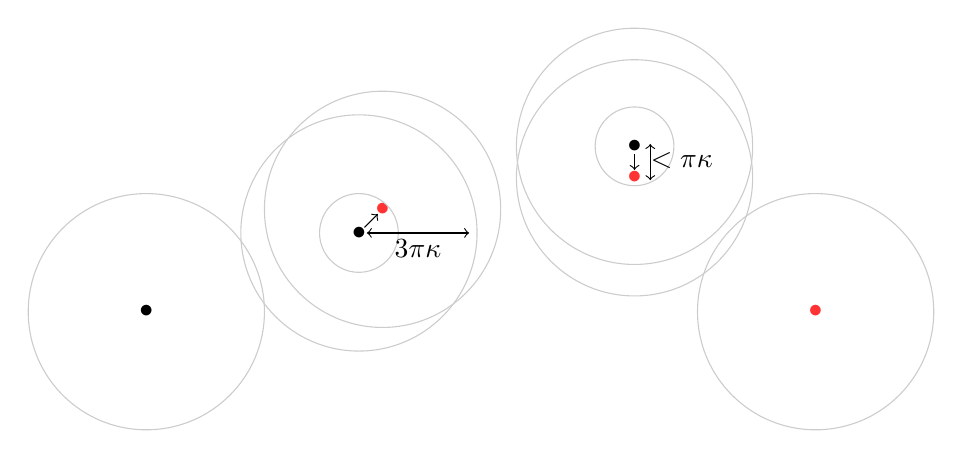
\begin{tikzpicture}
	% Pair 1
       	\draw[black] (0,0) node {$\bullet$} ;
	\draw[red!80] (.3,.3) node {$\bullet$} ; 
	\draw[->] 	(.07,.07)    	-- 	(.24,.24);
	\draw[black!20] (0,0) circle (1.5);
	\draw[black!20] (0,0) circle (0.5);
	\draw[black!20] (.3,.3) circle (1.5);
	\draw[<->]	(0.1,0)    	-- 	(1.4,0);
	\draw (0.75,-0.2)  node {$3\pi \kappa$};
	% Pair 2
	\draw[black] (3.5,1.1) node {$\bullet$} ;
	\draw[red!80] (3.5,0.7) node {$\bullet$} ; 
	\draw[->] 	(3.5,1.0)    	-- 	(3.5,0.8);
	\draw[black!20] (3.5,1.1) circle (1.5);
	\draw[black!20] (3.5,1.1) circle (0.5);
	\draw[black!20] (3.5,.7) circle (1.5);
	\draw[<->] 	(3.7,1.13)    	-- 	(3.7,0.67);
	\draw (4.1,0.92)  node {$<\pi \kappa$};
	% single black
	\draw[black] (-2.7,-1) node {$\bullet$} ;
	\draw[black!20] (-2.7,-1) circle (1.5);
	% single red
	\draw[red!80] (5.8,-1) node {$\bullet$} ;
	\draw[black!20] (5.8,-1) circle (1.5);
\end{tikzpicture}
        }
\caption{Configuration in dimension $2$ satisfying hypotheses of \thref{pairsdiracs}. The initial $\rho_0$ and final $\rho_1$ measures are composed of the black and red Dirac measures, respectively. At least 1 couple of spheres of radius $3\pi \kappa$ do not intersect for each pair of systems. We show that in that case, the geodesic is the sum of two travelling Dirac solutions (for the pairs), an on-place decreasing Dirac measure (single black) and an on place increasing Dirac measure (single red).}
\label{fig: matchingdiracs}
\end{figure}

\begin{proof}
Again we choose $\kappa=1$ without loss of generality. As for now, assume that all masses $h^i_0, h^i_1$ are strictly positive, the case of vanishing masses, i.e.\ ``single'' Dirac measures, will be fixed at the end of the proof. We aim at building an optimality certificate $\varphi \in C^1([0,1]\times \Om)$ for the candidate geodesic of the Theorem. Hence $\varphi $ should satisfy, for all $(t,x)\in [0,1]\times \Om$,
\[
\D_t \varphi +\frac12 \left( |\nabla \varphi| ^2 +  \varphi^2 \right) \leq 0
\]
and for all $t\in [0,1]$, for all $i\in \{ 1, \dots , N \}$ :
\[
\quad 
\begin{cases}
\nabla \varphi(x^i(t),t) = (x^i)'(t) \\
\varphi(x^i(t),t)=(h^i)'(t)/h^i(t) \\
\D_t \varphi +\frac12 \left( |\nabla \varphi |^2 + \varphi^2 \right) = 0 \quad  \text{for points of the form $(t,x^i(t))$}.
\end{cases}
\]

We introduce for $i\in \{1,\dots N\}$, the certificates $\varphi^i$ for the geodesics between each couple of Dirac measures $(h^i_0 \delta_{x^i_0}, h^i_1 \delta_{x^i_1})$ as defined in equation \eqref{certifddim}. The three parameters describing $\varphi^i$ are denoted $t^i_1, t^i_2$ and $\theta^i$. As $\theta^i$ is only defined up to translations, we decide from now on that $\theta^i$ is the unique such translation satisfying $\max\{ \vert x^i_0-\theta^i \vert, \vert x^i_1-\theta^i \vert \}< \pi$, which exists under our assumption that $|x_0^i - x_1^i|<\pi$. Thus, from the hypotheses in the Theorem, we have that $\min_{i \neq j}\{\vert \theta^i- \theta^j \vert \} > 4 \pi$. Now consider the \emph{binding} functions, defined for $i \in \{1,\dots,N \}$ by
\[
\varphi^i_b(t,x)=-\frac{1}{t-t^i_2} \cos(\vert x-\theta^i \vert ) + \frac{1}{t-t^i_2}. 
\]
Each $\varphi^i_b$ is in phase with $\varphi^i$ and satisfies 
\[
\varphi^i_b(t,\pi u + \theta^i)=\frac{2}{t-t_2^i}=\varphi^i(t,\pi u+ \theta^i) 
\quad \text{ and } \quad
\varphi^i_b(t,2\pi u+ \theta^i)=0
\]
for all $u\in \R^d$, $\vert u \vert = 1$ and $t\in[0,1]$. Also they are solutions to the equation $\D_t \varphi^i_b +\frac12 \left( (\nabla \varphi^i_b )^2 + (\varphi^i_b)^2 \right) = 0$. Now, as the constant zero function is a solution of this p.d.e too, we introduce
\begin{equation*}
\varphi(t,x)=
\begin{cases}
\varphi^i (t,x) & \text{if }  \vert x - \theta^i \vert \leq \pi \\
\varphi^i_b (t,x) & \text{if }  \vert x - \theta^i \vert \leq 2\pi  \text{ and } \vert x - \theta^i \vert > \pi\\
0 & \text{ otherwise.}
\end{cases}
\end{equation*}
Under the hypotheses of the Theorem, only one condition is met at a time so this function is well defined. It belongs to $C^1([0,1]\times \Om)$ because the bindings are located where the gradients vanish, on the extrema of cosines. See Figure \ref{figure certificate} to picture how the bindings are performed between the $\varphi^i$s. By construction, all hypotheses are fulfilled so that $\varphi$ be an optimality and uniqueness certificate.

Now if one or more of the $h^i_0$ or $h^i_1$ vanish, the same reasoning as in the proof of \thref{2diracs} allows to compute the distance between $\rho_0$ and $\rho_1$ (by an upper and lower bound, making the mass of vanishing Dirac measures tend to zero), and all that remains is to see that replacing the travelling Dirac solution by a Hellinger geodesic for single Dirac measures reaches that cost. 
\end{proof}

\begin{figure}%[ht]
\centering
 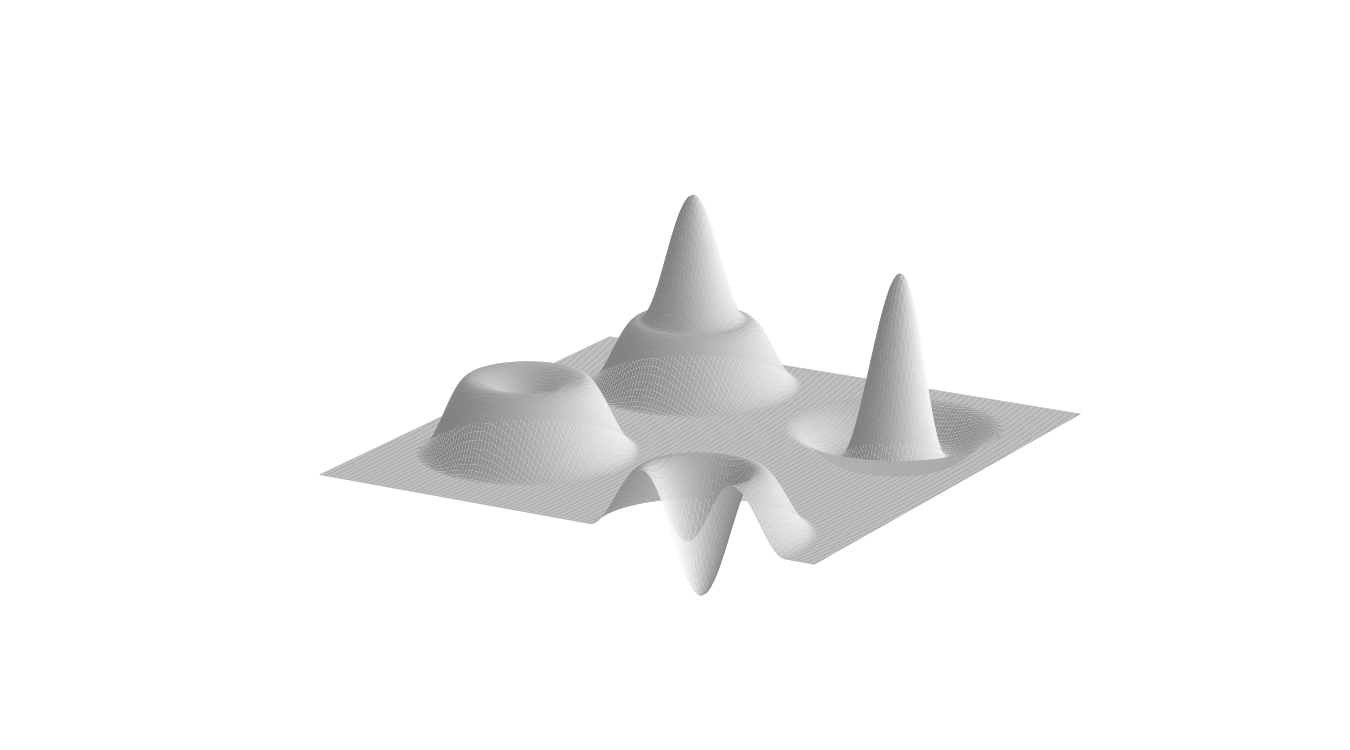
\includegraphics[trim=3cm 3cm 3cm 3cm, width=.7\linewidth]{images/certificate_dec2}%  ,clip,trim=15cm 10cm 15cm 15cm
 \caption{Example of an optimality certificate for $4$ pairs of Dirac measures, in the case $d=2$ at fixed $t$. The centers of the bumps are the $\theta^i$s. At the position $(t,x_i(t))$ of a travelling Dirac solution, the gradient gives its speed and the height gives its rate of growth.} 
 \label{figure certificate}
\end{figure}

%%%%%%%%%%%%%%%%%%%%%%%%%%%%%

% !TEX root = ../InterpolatingOTFR.tex

\section{Numerical results}
\label{sec-numerics}

This section presents a numerical implementation of the computation of geodesics for our metric. The source code to reproduce these results is available online\footnote{\url{https://github.com/lchizat/optimal-transport/}}.

\subsection{Discretization}

The numerical resolution of the dynamical optimal transport problem is often performed with first order methods using proximal splitting algorithms (\cite{benamou2000computational}, \cite{papadakis2014optimal}).  These methods extend with no difficulties to the case of transport with sources, as long as the proximal operator of the new functional can be easily computed. In order to compare a few models of optimal transport with source, we implemented a Douglas-Rachford proximal splitting algorithm on a staggered grid, in the footsteps of \cite{papadakis2014optimal}. The introduction of the source term comes with a few adjustments so we describe the numerical method that we implemented, in the case of a transport problem in 1-D for simplicity (but the scheme works in arbitrary dimension).

\paragraph{Centered and staggered grids.}

\begin{figure}
 \centering
  \resizebox{0.40\linewidth}{!}{
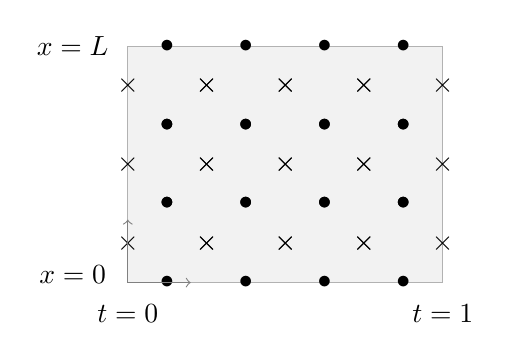
\begin{tikzpicture}
	\filldraw[color=black!30, fill=black!5] (-.5,-.5) rectangle (3.5,2.5);
	\foreach \x in {0,...,3}
   	 \foreach \y in {0,...,2} 
	 {
	\pgfmathparse{\x+0.5}\let\a\pgfmathresult
	\pgfmathparse{\y+0.5}\let\b\pgfmathresult
	\pgfmathparse{\x-0.5}\let\c\pgfmathresult
	\pgfmathparse{\y-0.5}\let\d\pgfmathresult
       	\draw[black,minimum size=5pt] (\x,\y) node {$\blacksquare$} ;
	\draw (\a,\y) node {$\times$} ; %[red!80]
	\draw  (\x,\b) node {$\bullet$} ; 
	\draw  (\c,\y) node {$\times$} ; 
	\draw  (\x,\d) node {$\bullet$} ; 
	}
	
	\draw[->, black!50] 	(-.5,-.5)    	-- 	(-.5,.3);
	%\draw       	(-1.4,1.) 	node {Space};
	\draw	(-1.2,-.4) node {$x=0$};
	\draw	(-1.2,2.5) node {$x=L$};
	
	\draw[->,black!50] 	(-.5,-.5) 	-- 	(.3,-.5);
	%\draw       	(1.5,-.9) 	node {Time};
	\draw 	(-.5,-.9)  	node {$t=0$};
	\draw 	(3.5,-.9) 	node {$t=1$};
\end{tikzpicture}
        }
\caption{($\blacksquare$) centered and ($\times$, $\bullet$) staggered grids. The grey rectangle is the space-time domain and here $N=3$, $T=4$.}
\label{fig: grids}
\end{figure}

%\todo{Gab: why not taking $L=1$ ?}

We consider the space domain $[0,L]$ and the time domain $[0,1]$. We denote $N$ the number of dicretization points in space and $T$ the number of discretization points in time. The centered grid is an equidistant discretization of the interior of the space-time domain $[0,L] \times [0,1]$, namely
\[
\mathcal{G}_c = \left\{ \left( x_i=L\frac{i-1/2}{N}, t_j=\frac{j-1/2}{T} \right): 1 \leq i \leq N, \, 1 \leq j \leq T \right\}
\]
and the variable discretized on the centered grid are denoted
\[
V = (\rho,\M,\Z) \in \mathcal{E}_c = (\R^{\mathcal{G}_c })^3.
\]
Remark that the boundaries are not included in the centered grid. There are as many staggered grids as there are dimensions, defined as
\[
\mathcal{G}_s^x = \left\{ (x_i = L\frac{i-1}{N}, t_j=\frac{j-1/2}{T}) :  1\leq i\leq N+1, \, 1\leq j \leq T \right\}\, ,
\]
\[
\mathcal{G}_s^t = \left\{ (x_i = L\frac{i-1/2}{N}, t_j=\frac{j-1}{T}) :  1\leq i\leq N, \, 1\leq j \leq T+1 \right\}\, , 
\]
and the variables discretized on the staggered grid are denoted by
\[
U = (\bar{\rho},\bar{\M},\bar{\Z}) \in \mathcal{E}_s = \R^{\mathcal{G}_s^t }\times \R^{\mathcal{G}_s^x }\times \R^{\mathcal{G}_c } .
\]
The source $\Z$ is discretized on the centered grid because there is no differentiation operator acting on this variable in the definition of the continuity constraint. Figure \ref{fig: grids} gives an illustration of the centered and staggered grids.

%%
\paragraph{Discrete continuity constraint.}
The discrete continuity constraint with boundary conditions is defined as the set
\begin{equation}
\label{eq_discretecontinuity}
\mathcal{CE} = \left\{   U= (\bar{\rho},\bar{\M},\bar{\Z}) \in \mathcal{E}_s :  AU = f_0 ,\, A = \left[
\begin{array}{c} 
\div - s_z \\ \hline 
s_b
\end{array}
\right]  , \, f_0 = \left[
\begin{array}{c}  
0  \\ \hline 
b_0
\end{array}
\right]  \right\}
\end{equation}
where $s_z : U \mapsto \bar{\zeta}$, $s_b$ selects the values of $U$ on the boundaries of the staggered grids and $b_0$  is a vector containing $\rho_0$, $\rho_1$ and zeros for the Neumann boundary conditions. The divergence operator $\div$ only acts on the components $(\bar{\rho},\bar{\M})$ of $U$, takes its values on the centered grid and is defined for $U\in \mathcal{E}_s$ as 
\[
\div(U)_{i,j} = \frac{N}{L} (\bar{\M}_{i+1,j}-\bar{\M}_{i,j}) + T (\bar{\rho}_{i,j+1}-\bar{\rho}_{i,j}) \, .
\]

%%%%%%%%%%%%%%%%%%%%%%
%%%%%%%%%%%%%%%%%%%%%%
\paragraph{Discrete functional.}

First, we use \thref{rescaling} and bring ourselves back to the case $\kappa = 1$ by a space rescaling: this allows to obtain a simpler proximal operator. The discrete functional is defined, for $V \in \mathcal{E}_c$, as $\ifoncN(V) \defeq \sum_{k\in\mathcal{G}_c } f(\rho_k,\M_k,\Z_k)$ with 
\[
f(\rho_k,\M_k,\Z_k) \defeq \frac{|\M_k|^2 + \Z_k}{2\rho_k} \, .
\]

%%%%%%%%%%%%%%%%%%%%
\paragraph{Interpolation operator.}
Since the continuity constraint and the functional $\ifoncN$ are not defined on the same grid, we need to keep two variables $(U,V)\in \mathcal{E}_s \times \mathcal{E}_c$ and to add an interpolation constraint between them, i.e.\ we require $V=\mathcal{I}(U)$ where $I$ is the midpoint interpolation operator 
\[
I(U)_{i,j} = \left( \frac{\bar{r}_{i,j+1}+\bar{r}_{i,j}}{2},\frac{\bar{m}_{i+1,j}+\bar{m}_{i,j}}{2},\bar{z}_{i,j} \right) \, .
\]

%%%%%%%%%%%%%%%%%%%%

\paragraph{Discrete optimization problem}
The discrete convex optimization problem that we aim to solve as an approximation of the continuous problem \eqref{dual} reads then
\begin{equation*}
\min_{U,V} \,  \ifoncN(V) + \iota_{\mathcal{CE}}(U) + \iota_{\{V=\mathcal{I}(U)\}} (U,V) \, .
\end{equation*}

%%%%%%%%%%%%%%%%%%%%%%
\subsection{Minimization algorithm}

\paragraph{Proximal methods and the Douglas Rachford algorithm.}

A popular class of first order methods for solving non-smooth convex optimization problems, so-called proximal splitting schemes, replaces the explicit gradient descent step by an implicit descent step using the so-called proximal operator. For a proper, convex, l.s.c.\ function $F$ defined on a Hilbert space $\mathcal{H}$ with values in $\R\cup +\infty$, the proximal operator is the single-valued map defined as
\[
	\prox_{\gamma F}(x) = \argmin_{\bar{x}\in \mathcal{H}} \frac12 \Vert x - \bar{x}  \Vert^2 + \gamma F(\bar{x}) \, .
\]
If $F$ is smooth, the optimality condition imply that $\bar{x} \defeq \prox_{\gamma F}(x)$ should satisfy $\bar{x} = x-\gamma \nabla F(\bar{x})$, justifying the common interpretation of the proximal operator as an implicit gradient step. 
%For the indicator function of a convex set, the proximal operator is the projection on this set.
A minimizer of $F$ can be found by successively applying the proximal operator, but for complicated functions without structure, computing the proximal operator can be as difficult as solving the whole minimization problem. 
However, if the function is the sum of simple terms, minimization can be performed by so-called \emph{proximal splitting} methods. 
%There are several ways to combine proximal operators in order to minimize the sum of functions. 
The one we implemented is the Douglas Rachford algorithm which allows to minimize the sum of two convex, proper, l.s.c.\ functions $G_1$ and $G_2$ with the following iterative scheme: choose two initial points $(z^{(0)},w^{(0)})\in \mathcal{H}^2$ and define the sequence
\begin{align*}
	w^{(l+1)} &= w^{(l)}+ \alpha (\prox_{\gamma G_1}(2z^{(l)}-w^{(l)})-z^{(l)}), \\
	z^{(l+1)} &= \prox_{\gamma G_2} (w^{(l+1)}) \, .
\end{align*}
If $0<\alpha<2$ and $\gamma >0$, one can show thant $z^{(l)} \rightarrow z^*$ a minimizer, see \cite{combettes2007douglas}. Depending on which functions we take as $G_1$ and $G_2$, we obtain various algorithms; in our code we used
\[
	G_1(U,V) = \iota_{\mathcal{CE}}(U) + \ifoncN(V) \quad \text{and} \quad G_2(U,V) = \iota_{V=\mathcal{I}(U)}(U,V) \, . 
\]
For a detailed review of proximal splitting algorithms, we refer the reader to \cite{combettes2011proximal}. Let us now compute the proximal operators.

%%%%%%%%%%%%%%%%%%%%%%%%%%%
\paragraph{Computing $\prox_{\gamma \ifoncN}$.}

The proximal operator of the functional $\ifoncN$ can be computed in closed form. The following result is a direct adaptation of \cite{papadakis2014optimal}.

\begin{proposition}
One has
\[
\forall \, V \in \mathcal{E}_c, \quad \prox_{\gamma \ifoncN}(V) = \left( \prox_{\gamma \foncN}(V_k)\right)_{k \in \mathcal{G}_c}
\]
where, for all $(\tilde{\rho},\tilde{\M}, \tilde{\Z}) \in \R \times \R^d \times \R$,
\[
\prox_{\gamma \foncN}(\tilde{\rho},\tilde{\M}, \tilde{\Z})  =
\begin{cases}
 \left( \rho^*, \frac{\rho^* \, \tilde{\M}}{\rho^* + \gamma},\frac{\rho^* \, \tilde{\Z}}{\rho^* + \gamma} \right) & \text{if $\rho^*>0$,}\\
 ( 0, 0, 0) & \text{otherwise},
\end{cases}
\]
and $\rho^*$ is the largest real root of the third order polynomial equation in $X$
\[
 P[X] = (X-\tilde{\rho})(X+\gamma)^2 - \frac{\gamma}{2} (|\tilde{\M}|^2+\tilde{\Z}^2) \, .
 \]
\end{proposition}

%%%%%%%%%%%%%%%%%%%%%%%%%%%
\paragraph{Computing $\proj_{\mathcal{CE}}$.}

The proximal operator of $\iota_{\mathcal{CE}}$ is the projection on the affine set $\mathcal{CE}$, which can be computed for $U \in \mathcal{E}_s$ as
 \begin{eqnarray}
\mathcal{P}_\mathcal{CE} (U) & = & U + A^* (A A^*)^{-1}(b_0 -AU) \\
& = & \mathcal{P}_B (U) - (Id-I_b)(s_z^* -\div^*) S^{-1} (s_z - \div ) (\mathcal{P}_B (U))
\end{eqnarray}
where $S=(\div - s_z)(Id - s_b^* s_b)(-\nabla - s_z^*)$ is the Schur complement of $AA^*$, $I_b$ is the identity on the boundaries on zero everywhere else and $\mathcal{P}_B$ is the projection on the boundary constraints. Given $p$, we can find $u$ satisfying $Su=p$ by solving $\Delta u -u + p=0$ on the centered grid with Neumann boundary conditions (on the staggered grids). In the Fourier domain, this equation reads
\[
\left[ 1 + (2- 2\cos( \pi m /N) )N/L + (2- 2\cos( \pi n/T) )T \right]   \hat{u}[m,n] = \hat{p}[m,n] \, .
%\left( 5 -2 \cos (2i\pi m/N) -2 \cos (2i\pi n/T) \right) \hat{u}[m,n] = h^2 \hat{p}[m,n] \, . %less general
\]
The DCT-II transform (with inverse DCT-III ) which coefficients are given by
\[
\hat{u}[k] = \sum_{n=1}^{N} u[n] \cos \left[ \frac{\pi}{N} (n+\frac{1}{2})k  \right]
\]
is adapted to our boundary conditions.

%%%%%%%%%%%%%%%%%%%%%%%%%%%%
\paragraph{Compute $\proj_{V = \mathcal{I}(U)}$.}
The projection is given for all couples $(U_0,V_0) \in (\mathcal{E}_s, \mathcal{E}_c )$ by 
\[
\proj_{V = \mathcal{I}(U)} (U_0,V_0) = (U^*, \mathcal{I}(U^*))
\]
with $U^*=Q^{-1}(U_0+\mathcal{I}^*V_0)$ and $Q=Id+\mathcal{I}^*\mathcal{I}$.
As $Q$ is a tridiagonal matrix, LU factorization techniques allow to efficiently invert the system.
%%%%%%%%%%%%%%%%%%%%%%%%%%%%
%\paragraph{Other proximal operators.}
%[???]


%%%%%%%%%%%%%%%%%%%%%%%%%
%%%%%%%%%%%%%%%%%%%%%%%%%
\subsection{Experiments}
%%%%%%%%

\begin{figure}[hbt]
 \centering
%
\begin{subfigure}{0.5\linewidth} 
\centering
 \resizebox{1.\linewidth}{!}{
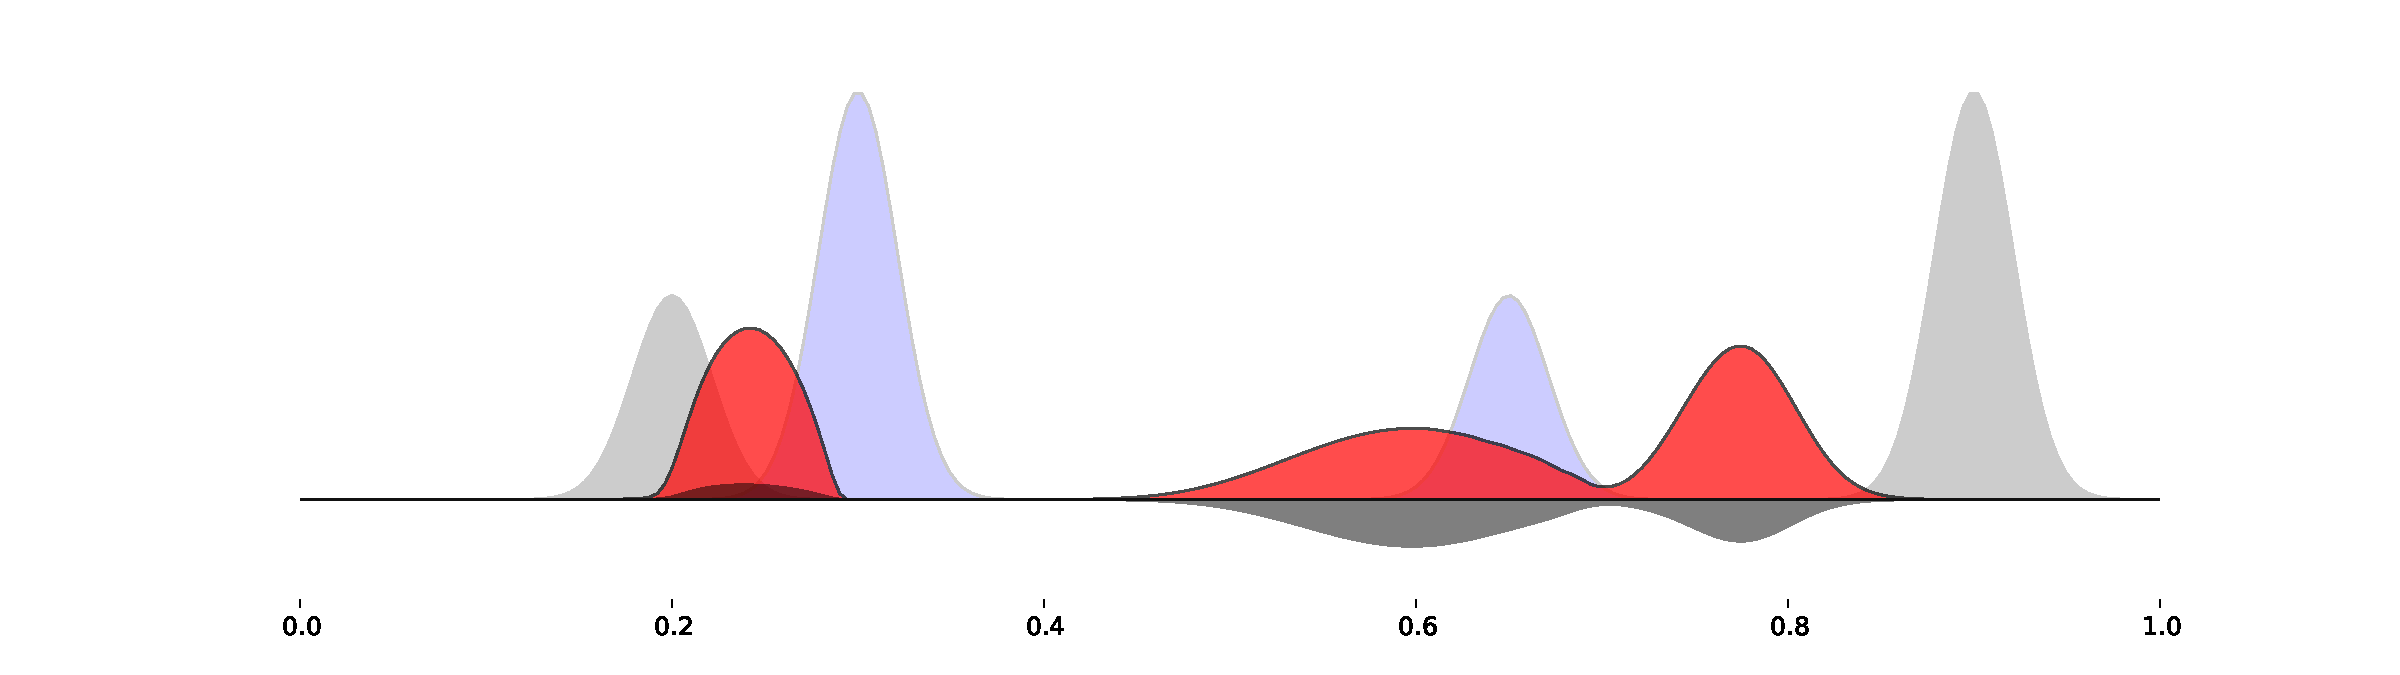
\includegraphics{images/gaussian_p2q0}
}
\caption{Standard transport $W_2$}
\label{subW2}
\end{subfigure}%
%
\begin{subfigure}{0.5\linewidth} 
\centering
  \resizebox{1.\linewidth}{!}{
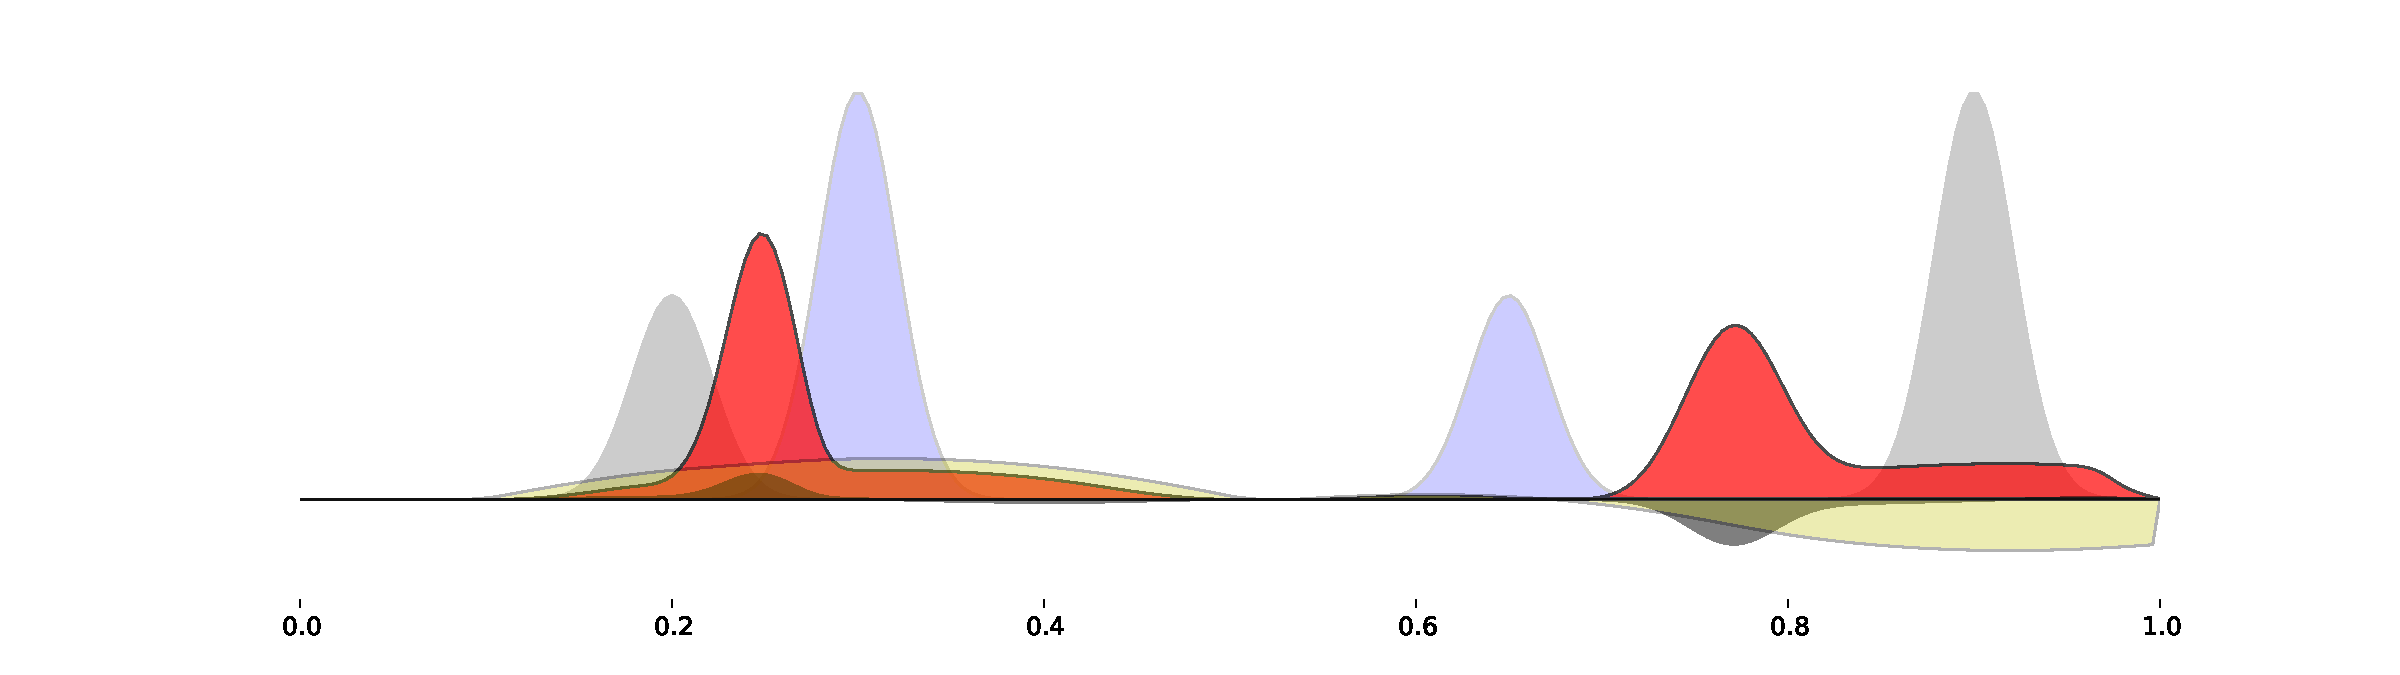
\includegraphics{images/gaussian_p2L2}
}
\caption{$L^2$ penalization on the source}
\label{subL2}
\end{subfigure}%

\begin{subfigure}{0.5\linewidth} 
\centering
 \resizebox{1.\linewidth}{!}{
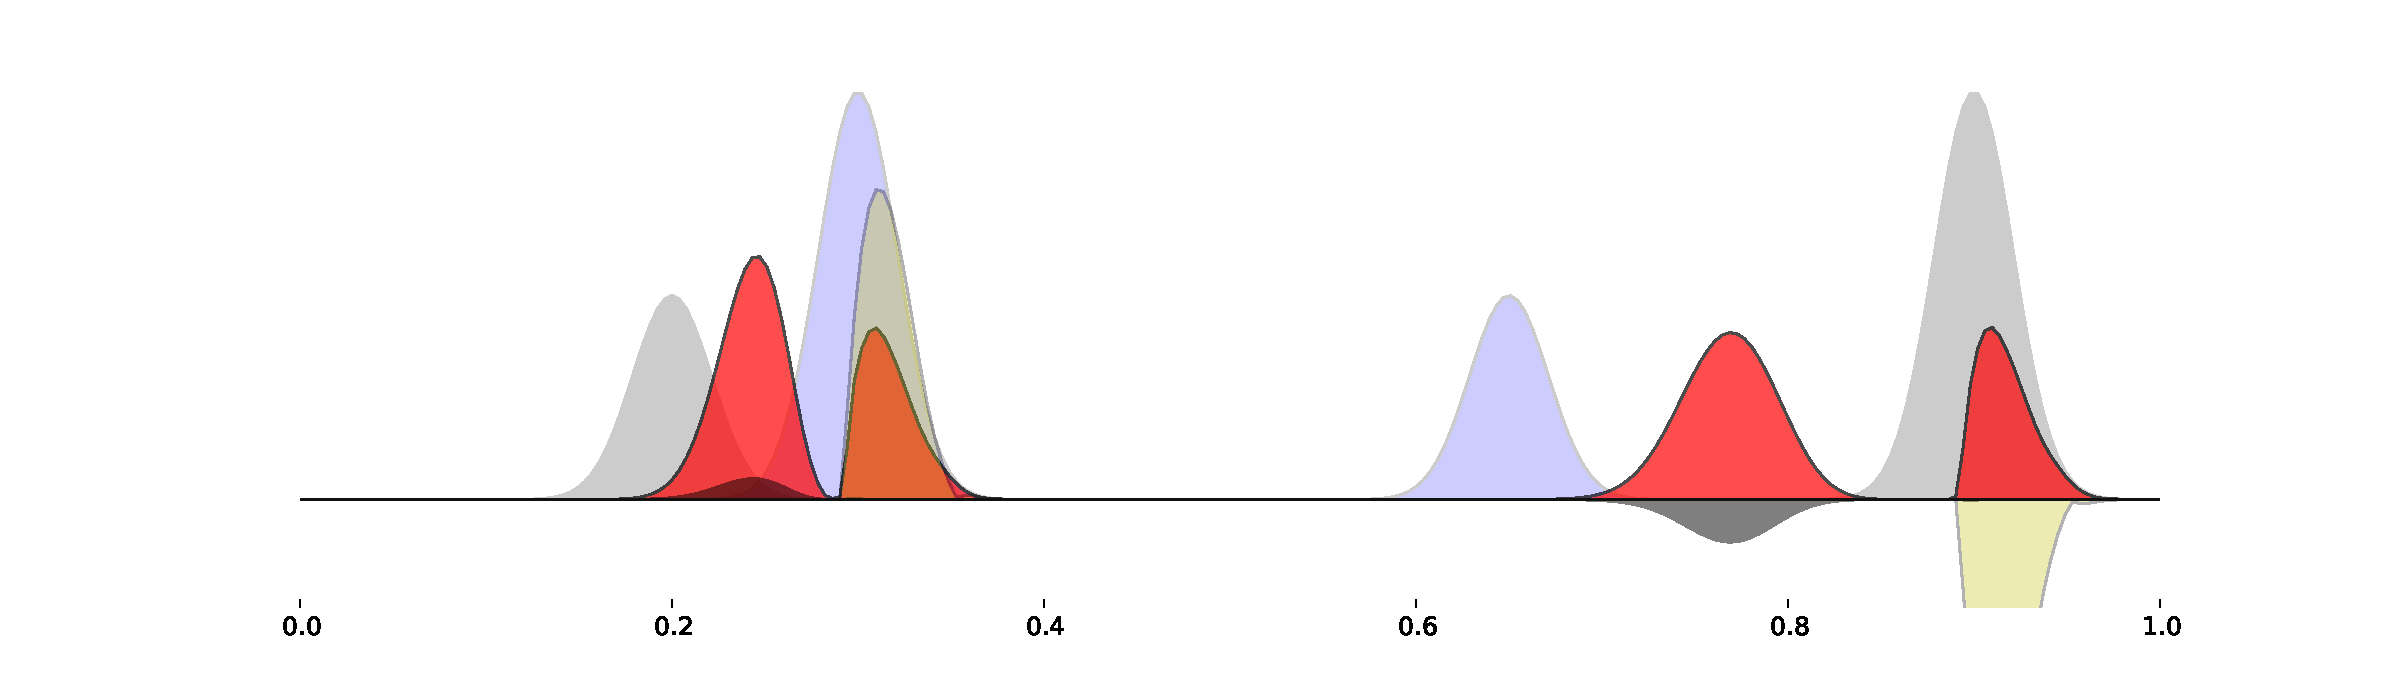
\includegraphics{images/gaussian_p2q1}
}
\caption{Partial transport with $c_l=0.3$}
\label{subPT1}
\end{subfigure}%
%
\begin{subfigure}{0.5\linewidth} 
\centering
 \resizebox{1.\linewidth}{!}{
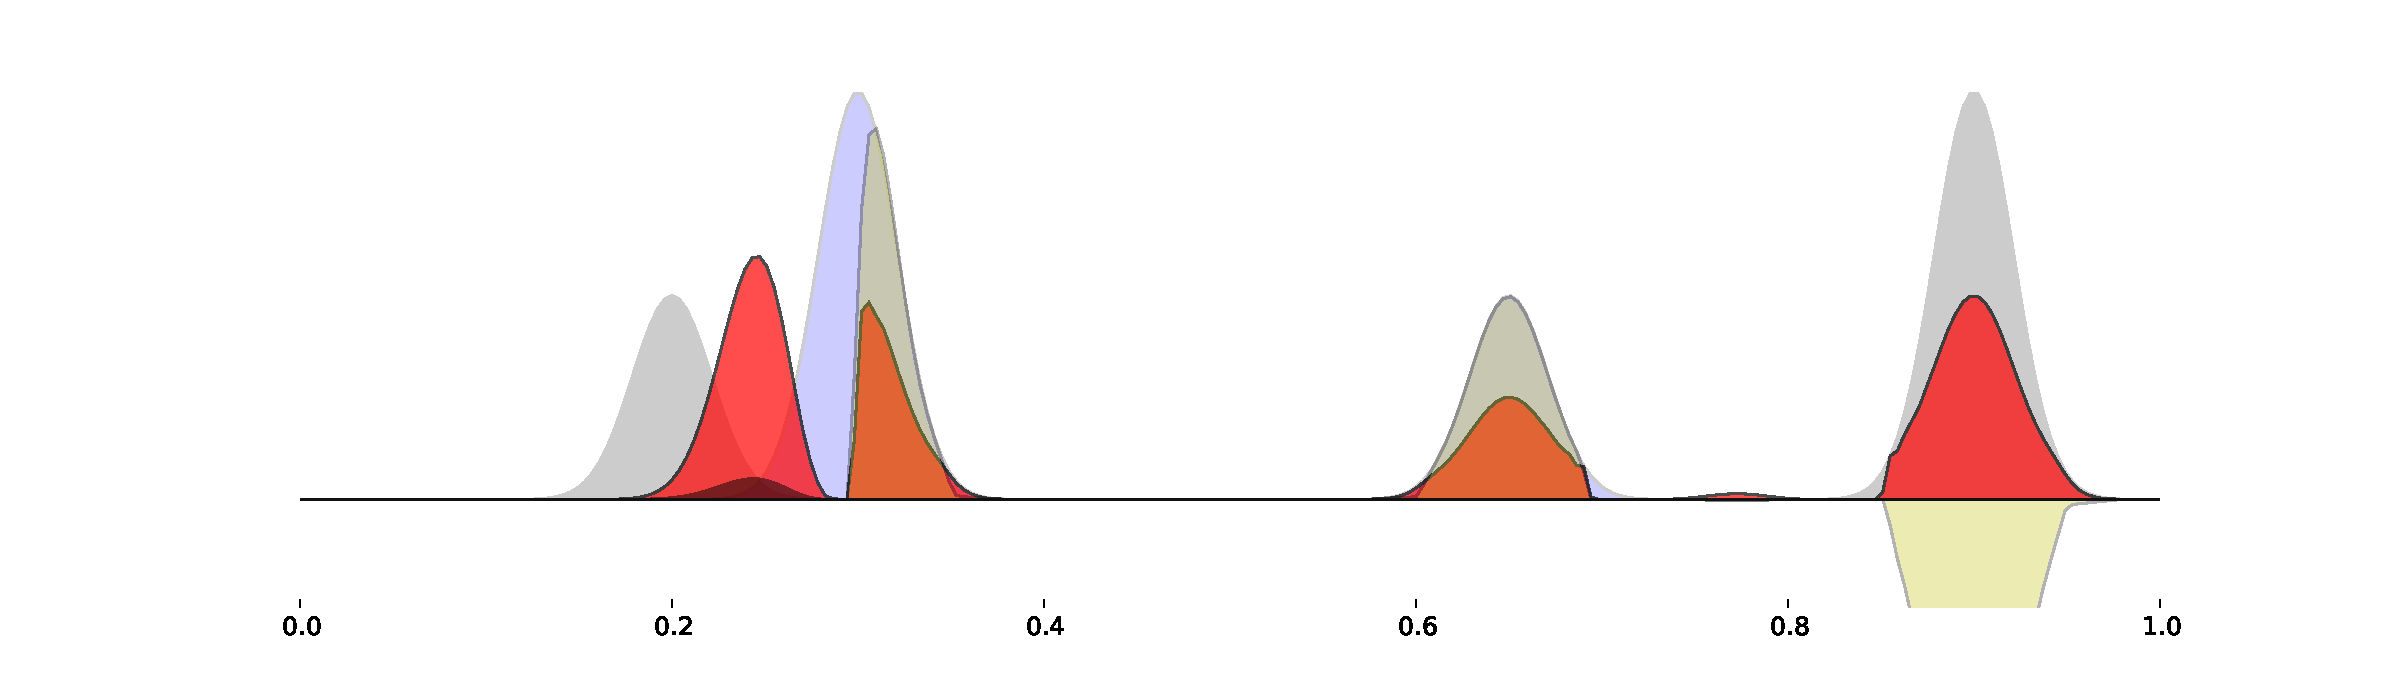
\includegraphics{images/gaussian_p2q1_small}
}
\caption{Partial transport with $c_l = 0.15$}
\label{subPT2}
\end{subfigure}

\begin{subfigure}{0.5\linewidth} 
\centering
  \resizebox{1.\linewidth}{!}{
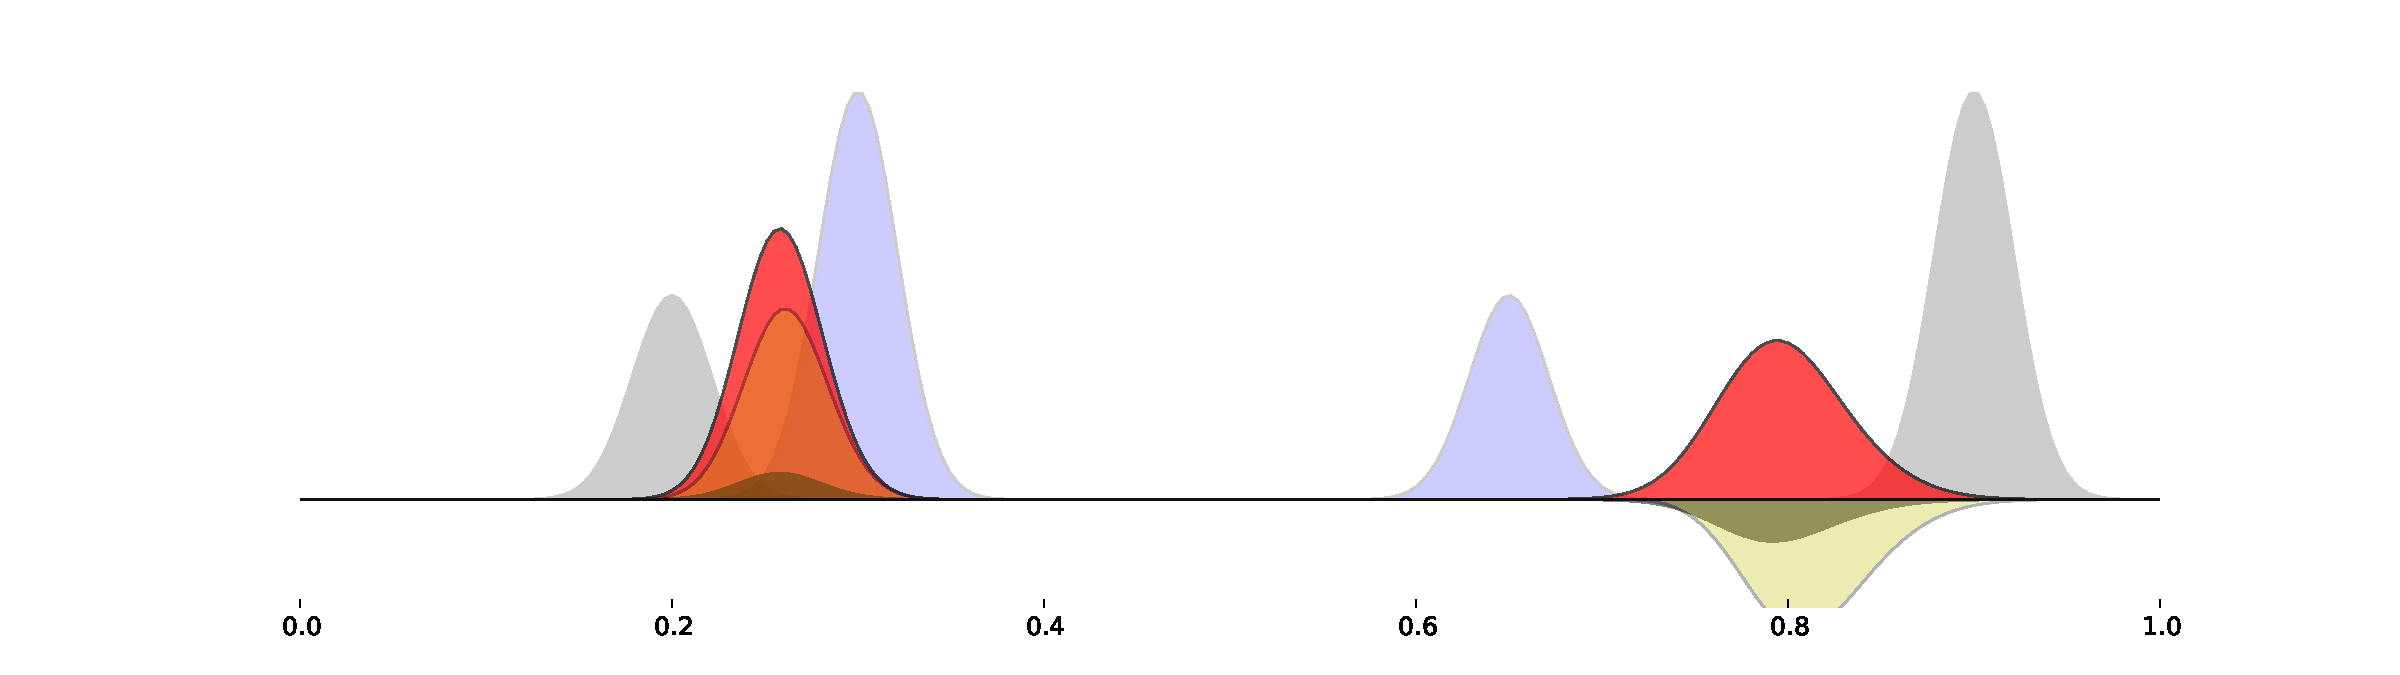
\includegraphics{images/gaussian_p2q2}
}
\caption{$\WF_{\kappa}$ with $c_l =0.3$}
\label{subWF1}
\end{subfigure}%
%
\begin{subfigure}{0.5\linewidth} 
\centering
  \resizebox{1.\linewidth}{!}{
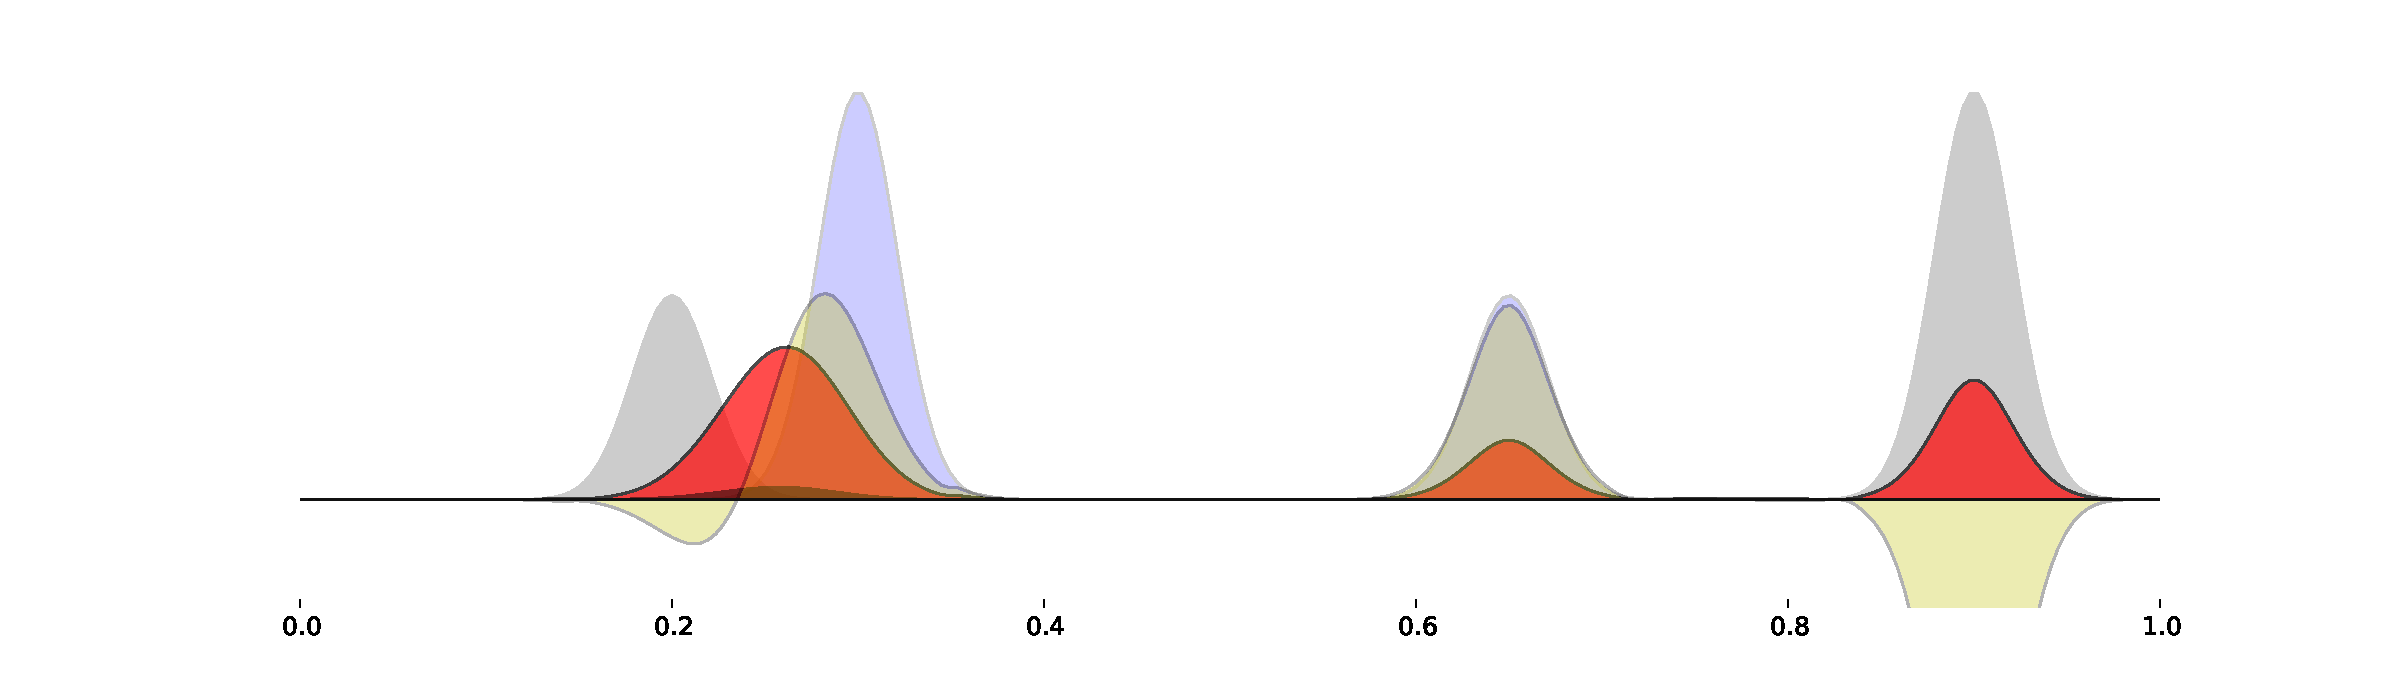
\includegraphics{images/gaussian_p2q2_small}
}
\caption{$\WF_{\kappa}$ with $c_l = 0.15$}
\label{subWF2}
\end{subfigure}
\caption{Comparison of interpolations for densities on the segment $[0,1]$:  $\rho_0$ (gray),  $\rho_1$ (blue),  $\rho_{t=1/2}$  (red), $\omega_{t=1/2}$ (black),  $\zeta_{t=1/2}$ (yellow). We indicate by $c_l$ the theoretical maximum distance a Dirac can travel, which is a function of $\kappa$.}
\label{fig:gaussians}
\end{figure}

%%%
\paragraph{Transport of Gaussian bumps.}

Let us first explore a synthetic case where the initial and final measures have the same mass. This case is shown on Figure \ref{fig:gaussians}. 
The initial and the final measures are both composed of two Gaussian densities of mass $1$ and $2$ supported on the segment $\Om=[0,1]$. The modes of the bumps are located at, from left to right, $0.2$, $0.3$, $0.65$ and $0.9$. The problem is discretized with $N=256$ samples in space and $T=11$ samples in time. The peculiar location of the Gaussian bumps allows to highlight the variations of the behavior of the geodesics, which is highly dependent on the metric and on the parameter $\kappa$. 
%
For the $W_2$ geodesic (Figure \ref{subW2}), the rightmost grey bump is split in half and a part of it travels to the left side of the graph, giving a interpolated measure which, for some applications, is not so natural. The effect of a non-homogeneous functional is visible on Figure \ref{subL2}, where we penalized the $L^2$ norm of the source $\Z$ in the functional. Non-homogeneity makes the density matter: in this case, the source is spread because low densities are favored. 
%
Consider now the partial transport geodesics: on Figure \ref{subPT1}, we fixed the maximum distance mass can travel to $2\kappa=0.3$, while on Figure \ref{subPT2}, that distance is $2\kappa=0.15$. We observe, as expected, that the domain $\Om=[0,1]$ is split in an active and an inactive set. Also note that as the $TV$ cost is not strictly convex, geodesics are not unique and what happens in the inactive set depends on the initialization of the algorithm.
%
Finally, Figures \ref{subWF1} and \ref{subWF2} display the geodesics at $t=1/2$ for the $\WF_{\kappa}$ metric with the \emph{cut locus} distances set, respectively, at $\pi \kappa=0.3$ and $\pi \kappa = 0.15$. Note that there is a slight similarity between the configuration here and the hypotheses of \thref{pairsdiracs}, and the observed behavior can be expected if we extrapolate the conclusions of that Theorem. In the first case, we obtain a geodesic consisting of two travelling bumps which inflate or deflate. While in the second configuration, only one bump travels as $\pi \kappa$ is now smaller than the distance between the two bumps at the right. 

%%%%%%%%%%%%%%%%%%%
% SYNTHETIC
%%%%%%%%%%%%%%%
\paragraph{Synthetic 2D experiments.}
We now turn our attention to a synthetic example on the domain $\Om=[0,1]^2$. The initial density $\rho_0$ is the indicator of the ring of center $(\frac12, \frac12)$, internal diameter $0.5$ and external diameter $0.7$. The final density $\rho_1$ is the pushforward of $\rho_1$ by a random smooth map and thus $\rho_0(\Om)=\rho_1(\Om)$. The domain is discretized on a centered grid of $64\times 64$ samples in space and $T=12$ samples in time. We compare on Figure \ref{fig: synthetic rho} the geodesics for four different metrics: $d_{FR}$, $W_2$, partial optimal transport (with $2\kappa=0.2$) and $\WF_{\kappa}$ (with $\kappa \pi = 0.4$). Notice that the two first rows thus show the limit geodesics for $\WF_{\kappa}$ when $\kappa$ tends to $0$ or $+\infty$ (see \thref{limitmodels}).

Figure \ref{fig: synthetic details} helps to better understand the geodesics. On the top row, the velocity field shows that the $W_2$ geodesic transports a lot of mass to the bottom left protuberance. On the contrary, metrics allowing local variations of mass (partial transport and $\WF_{\kappa}$), attenuate the component of the velocity field which is tangential to the ring, behavior which is more consistent with the intuitive solution. Finally, by looking at the source maps in the bottom row, we see the inactive sets of partial optimal transport with well defined edges and how this behavior strongly differs to that of $\WF_{\kappa}$ geodesics.

Figure \ref{fig: synthetic rho distance} displays another experiment intended to illustrates how the geodesics behave when a lot of transport is involved. The measures $\rho_0$ and $\rho_1$ have same total mass, the domain $\Om=[0,1]^2$ is discretized on a centered grid with $44 \times 44$ samples in space and $T=12$ samples in time. We show the geodesics for $W_2$, partial optimal transport (with $2\kappa=0.5$) and $\WF_{\kappa}$ (with $\kappa \pi = 0.5$).


\begin{figure}
 \centering
  \resizebox{1.0\linewidth}{!}{
\begin{tikzpicture}
\filldraw[color=black!5, fill=black!5] (-1.5,-1.) rectangle (.5,1);
\filldraw[color=black!5, fill=black!5] (11.5,-1.) rectangle (13.5,1);
\node (1r1) at (-0.5,0) {
\includegraphics{images/circle_p2q0_r1}};
% p0q2
\node (3r2) at (2,2.25) {
\includegraphics{images/circle_p0q2_r3}};
\node (3r3) at (4,2.25) {
\includegraphics{images/circle_p0q2_r5}};
\node (3r4) at (6,2.25) {
\includegraphics{images/circle_p0q2_r7}};
\node (3r5) at (8,2.25) {
\includegraphics{images/circle_p0q2_r9}};
\node (3r6) at (10,2.25) {
\includegraphics{images/circle_p0q2_r11}};
% p2q0
\node (0r2) at (2,.75) {
\includegraphics{images/circle_p2q0_r3}};
\node (0r3) at (4,.75) {
\includegraphics{images/circle_p2q0_r5}};
\node (0r4) at (6,.75) {
\includegraphics{images/circle_p2q0_r7}};
\node (0r5) at (8,.75) {
\includegraphics{images/circle_p2q0_r9}};
\node (0r6) at (10,.75) {
\includegraphics{images/circle_p2q0_r11}};
% p2q1
\node (1r2) at (2,-.75) {
\includegraphics{images/circle_p2q1_r3}};
\node (1r3) at (4,-.75) {
\includegraphics{images/circle_p2q1_r5}};
\node (1r4) at (6,-.75) {
\includegraphics{images/circle_p2q1_r7}};
\node (1r5) at (8,-.75) {
\includegraphics{images/circle_p2q1_r9}};
\node (1r6) at (10,-.75) {
\includegraphics{images/circle_p2q1_r11}};
%p2q2
\node (2r2) at (2,-2.25) {
\includegraphics{images/circle_p2q2_r3}};
\node (2r3) at (4,-2.25) {
\includegraphics{images/circle_p2q2_r5}};
\node (2r4) at (6,-2.25) {
\includegraphics{images/circle_p2q2_r7}};
\node (2r5) at (8,-2.25) {
\includegraphics{images/circle_p2q2_r9}};
\node (2r6) at (10,-2.25) {
\includegraphics{images/circle_p2q2_r11}};

\node (1r7) at (12.5,0) {
\includegraphics{images/circle_p2q0_r13}};

\draw[->] 	(1r1)    	-- 	(3r2);
\draw[->] 	(1r1)    	-- 	(0r2);
\draw[->]  	(1r1)    	-- 	(1r2);
\draw[->] 	(1r1)    	-- 	(2r2);
%\draw[dashed,color=black!30] (2,.9) --(10,0.9);
%\draw[dashed,color=black!30] (2,-1) -- (10,-1);
\draw[->]  	(3r6)    	-- 	(1r7);
\draw[->]  	(2r6)    	-- 	(1r7);
\draw[->] 	(0r6)    	-- 	(1r7);
\draw[->]  	(1r6)    	-- 	(1r7);
\draw[->]  	(-.5,-3)    	-- 	(12.5,-3);

\draw[dotted]        (2,0) -- (10,0);
\draw[dotted]        (2,-1.5) -- (10,-1.5);
\draw[dotted]        (2,1.5) -- (10,1.5);
\draw 	(-.5,-3.)  		node {$\bullet$};
\draw 	(-.5,-3.2)  		node {$t=0$};
\draw 	(12.5,-3.2)  	node {$t=1$};
\draw 	(6,-3.2)  	node {$t=0.5$};
\draw 	(-.5,-1.5)  	node {$\rho_0$};
\draw 	(12.5,-1.5)  	node {$\rho_1$};

\end{tikzpicture}
        }
\caption{Geodesics between $\rho_0$ and $\rho_1$ for four metrics:  Fisher-Rao (1st row),  $W_2$  (2nd row),  partial optimal transport (3rd row),  $\WF_{\kappa}$  (4th row).}
\label{fig: synthetic rho}
\end{figure}
%%%%%%%%%%%%%%%%%%%%%
%%%%%%%%%%%%%%%%%%%%%

\begin{figure}[ht]
 \centering
       
\begin{subfigure}{0.3\linewidth} 
\centering
 \resizebox{1.\linewidth}{!}{

\includegraphics[clip,trim=2cm 2cm 2cm 2cm]{images/circle_p2q0_v}
}
\caption{$W_2$}
\end{subfigure}%
%
\begin{subfigure}{0.3\linewidth} 
\centering
 \resizebox{1.\linewidth}{!}{
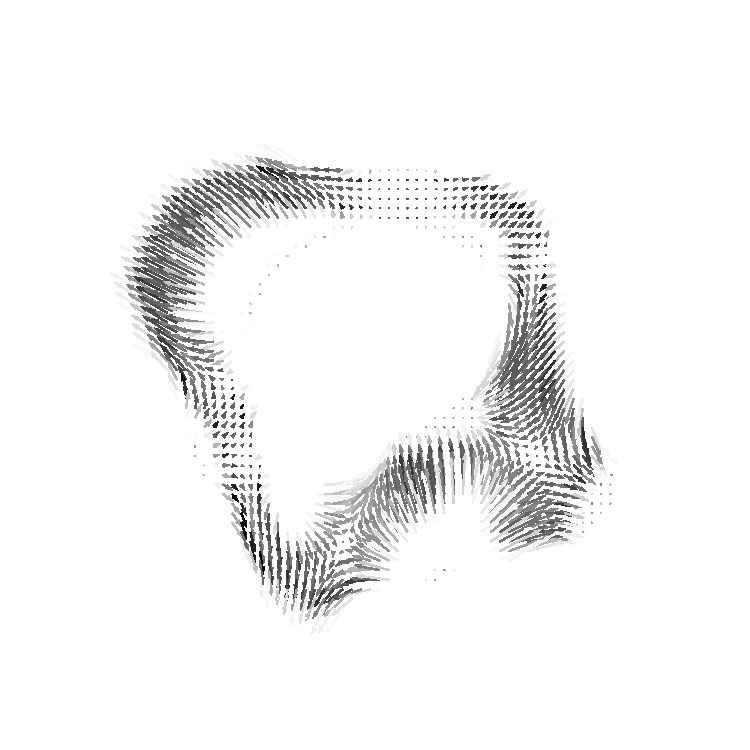
\includegraphics[clip,trim=2cm 2cm 2cm 2cm]{images/circle_p2q1_v}
}
\caption{Partial transport}
\end{subfigure}%
%
\begin{subfigure}{0.3\linewidth} 
\centering
  \resizebox{1.\linewidth}{!}{
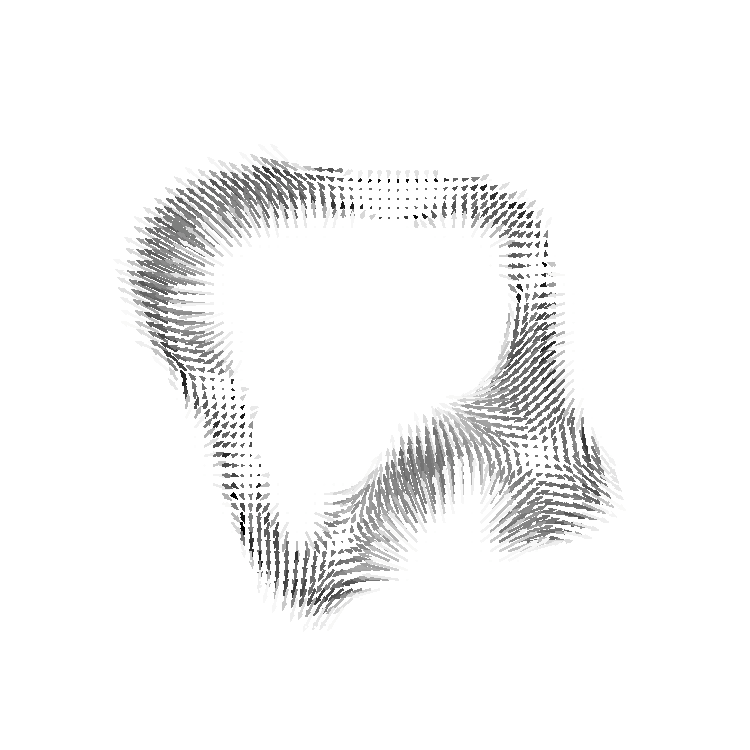
\includegraphics[clip,trim=2cm 2cm 2cm 2cm]{images/circle_p2q2_v}
}
\caption{$\WF_{\kappa}$}
\end{subfigure}

%
\begin{subfigure}{0.25\linewidth} 
\centering
 \resizebox{1.\linewidth}{!}{

\includegraphics[clip]{images/circle_p2q1_z6}
}
\caption{Partial transport}
\end{subfigure}%
%
\begin{subfigure}{0.25\linewidth} 
\centering
  \resizebox{1.\linewidth}{!}{

\includegraphics[clip]{images/circle_p2q2_z6}
}
\caption{$\WF_{\kappa}$}
\end{subfigure}

\caption{First row: velocity field $v = \omega/\rho$ at time $t=1/2$. The higher $\rho$, the darker the arrow. Second row: source $\zeta$ at time $t=1/2$. Blue stands for negative density and red for positive.}
\label{fig: synthetic details}
\end{figure}

\begin{figure}
 \centering
  \resizebox{1.0\linewidth}{!}{
\begin{tikzpicture}
\filldraw[color=black!5, fill=black!5] (-1.2,-1.45) rectangle (.2,-.05);
\filldraw[color=black!5, fill=black!5] (11.8,-1.45) rectangle (13.2,-.05);
\node (1r1) at (-0.5,-.75) {
\includegraphics{images/linevar/linevar_p2q0_r1}};
% p2q0
\node (0r2) at (2,.75) {
\includegraphics{images/linevar/linevar_p2q0_r3}};
\node (0r3) at (4,.75) {
\includegraphics{images/linevar/linevar_p2q0_r5}};
\node (0r4) at (6,.75) {
\includegraphics{images/linevar/linevar_p2q0_r7}};
\node (0r5) at (8,.75) {
\includegraphics{images/linevar/linevar_p2q0_r9}};
\node (0r6) at (10,.75) {
\includegraphics{images/linevar/linevar_p2q0_r11}};
% p2q1
\node (1r2) at (2,-.75) {
\includegraphics{images/linevar/linevar_p2q1_r3}};
\node (1r3) at (4,-.75) {
\includegraphics{images/linevar/linevar_p2q1_r5}};
\node (1r4) at (6,-.75) {
\includegraphics{images/linevar/linevar_p2q1_r7}};
\node (1r5) at (8,-.75) {
\includegraphics{images/linevar/linevar_p2q1_r9}};
\node (1r6) at (10,-.75) {
\includegraphics{images/linevar/linevar_p2q1_r11}};
%p2q2
\node (2r2) at (2,-2.25) {
\includegraphics{images/linevar/linevar_p2q2_r3}};
\node (2r3) at (4,-2.25) {
\includegraphics{images/linevar/linevar_p2q2_r5}};
\node (2r4) at (6,-2.25) {
\includegraphics{images/linevar/linevar_p2q2_r7}};
\node (2r5) at (8,-2.25) {
\includegraphics{images/linevar/linevar_p2q2_r9}};
\node (2r6) at (10,-2.25) {
\includegraphics{images/linevar/linevar_p2q2_r11}};

\node (1r7) at (12.5,-.75) {\includegraphics{images/linevar/linevar_p2q2_r13}};

%\draw[->] 	(1r1)    	-- 	(3r2);
\draw[->] 	(1r1)    	-- 	(0r2);
\draw[->]  	(1r1)    	-- 	(1r2);
\draw[->] 	(1r1)    	-- 	(2r2);
%\draw[dashed,color=black!30] (2,.9) --(10,0.9);
%\draw[dashed,color=black!30] (2,-1) -- (10,-1);
%\draw[->]  	(3r6)    	-- 	(1r7);
\draw[->]  	(2r6)    	-- 	(1r7);
\draw[->] 	(0r6)    	-- 	(1r7);
\draw[->]  	(1r6)    	-- 	(1r7);
\draw[->]  	(-.5,-3)    	-- 	(12.5,-3);

\draw[dotted]        (2,0) -- (10,0);
\draw[dotted]        (2,-1.5) -- (10,-1.5);
%\draw[dotted]        (2,1.5) -- (10,1.5);
\draw 	(-.5,-3.)  		node {$\bullet$};
\draw 	(-.5,-3.2)  		node {$t=0$};
\draw 	(12.5,-3.2)  	node {$t=1$};
\draw 	(6,-3.2)  	node {$t=0.5$};
\draw 	(-.5,-2.25)  	node {$\rho_0$};
\draw 	(12.5,-2.25)  	node {$\rho_1$};

\end{tikzpicture}
        }
\caption{Geodesics between $\rho_0$ and $\rho_1$ for three metrics: $W_2$ (1st row), partial optimal transport (2nd row),  $\WF_{\kappa}$ (3rd row). It is important to notice that $\rho_0$ is denser at the bottom left while $\rho_1$ is denser at the top right to better understand those geodesics.}
\label{fig: synthetic rho distance}
\end{figure}
%%%%%%%%%%%%%%%%%%%%%
%%%%%%%%%%%%%%%%%%%%%

%%%%%%%%%%%%%%%%%%%%%

%%%
\begin{figure}[ht]
 \centering
  \resizebox{1.0\linewidth}{!}{
\begin{tikzpicture}
\filldraw[color=black!5, fill=black!5] (-1.5,-1.25) rectangle (.5,1.25);
\filldraw[color=black!5, fill=black!5] (11.5,-1.25) rectangle (13.5,1.25);
\node (1r1) at (-0.5,0) {\includegraphics{images/brain_p2q2_r1}};

% p2q0
\node (0r2) at (2,1.25) {\includegraphics{images/brain_p2q2_r3}};
\node (0r3) at (4,1.25) {\includegraphics{images/brain_p2q2_r5}};
\node (0r4) at (6,1.25) {\includegraphics{images/brain_p2q2_r7}};
\node (0r5) at (8,1.25) {\includegraphics{images/brain_p2q2_r8}};
\node (0r6) at (10,1.25) {\includegraphics{images/brain_p2q2_r10}};
% p2q1
\node (1r2) at (2,-1.25) {\includegraphics{images/brain_p2q0_r3}};
\node (1r3) at (4,-1.25) {\includegraphics{images/brain_p2q0_r5}};
\node (1r4) at (6,-1.25) {\includegraphics{images/brain_p2q0_r7}};
\node (1r5) at (8,-1.25) {\includegraphics{images/brain_p2q0_r9}};
\node (1r6) at (10,-1.25) {\includegraphics{images/brain_p2q0_r11}};


\node (1r7) at (12.5,0) {\includegraphics{images/brain_p2q0_r13}};


\draw[->] 	(1r1)    	-- 	(0r2);
\draw[->]  	(1r1)    	-- 	(1r2);

\draw[dashed,color=black!30] (2,0) --(10,0.);
%\draw[dashed,color=black!30] (2,-1) -- (10,-1);


\draw[->] 	(0r6)    	-- 	(1r7);
\draw[->]  	(1r6)    	-- 	(1r7);
\draw[->]  	(-.5,-3)    	-- 	(12.5,-3);

%\draw[dotted]        (2,0) -- (10,0);
\draw 	(-.5,-3.)  		node {$\bullet$};
\draw 	(-.5,-3.2)  		node {$t=0$};
\draw 	(12.5,-3.2)  	node {$t=1$};
\draw 	(6,-3.2)  	node {$t=0.5$};
\draw 	(-.5,-1.5)  	node {$\rho_0$};
\draw 	(12.5,-1.5)  	node {$\rho_1$};

\end{tikzpicture}
        }
\caption{Geodesics between $\rho_0$ and $\rho_1$ for two metrics:   $W_2$ between rescaled densities (top row), $\WF_{\kappa}$ metric with $\pi\kappa=0.2$ (bottom row).}
\label{fig: brain interp}
\end{figure}

%
\begin{figure}
 \centering
       
\begin{subfigure}{0.3\linewidth} 
\centering
 \resizebox{1.\linewidth}{!}{
\includegraphics[clip,trim=2cm 1cm 2cm 1cm]{images/brain_p2q0_v_s3}
}
\caption{$v_{0.5}$ for $W_2$}
\label{fig: brain velo w2}
\end{subfigure}%
%
\begin{subfigure}{0.3\linewidth} 
\centering
 \resizebox{1.\linewidth}{!}{
\includegraphics[clip,trim=2cm 1cm 2cm 1cm]{images/brain_p2q2_v}
}
\caption{$v_{0.5}$ for $\WF_{\kappa}$}
\label{fig: brain velo wf}
\end{subfigure}%
%
\begin{subfigure}{0.33\linewidth} 
\centering
  \resizebox{1.\linewidth}{!}{
\includegraphics[clip,trim=0cm -0cm 0cm -0cm]{images/brain_p2q2_z}
}
\caption{$g_{0.5}$ for $\WF_{\kappa}$}
\label{fig: brain g wf}
\end{subfigure}

\caption{(a) and (b): velocity field $v=\omega/\rho$ for geodesics at time $t=1/2$. The higher $\rho_{0.5}$, the darker the arrow. (c) rate of growth $g=\Z/\rho$ at time $t=1/2$. Blue stand for negative density and red for positive and $g$ is set to zero when $\rho \approx 0$. Note that theoretically, (b) is the gradient field of (c).}
\label{fig: brain details}
\end{figure}

\paragraph{Biological images interpolation.}
Interpolating between shapes with varying masses is an important motivation for introducing this metric and is the object of our third and last numerical experiment. The initial and final densities $\rho_0, \rho_1$ are extracted form two segmented images of the same young brain taken at different times. This example is rather challenging for image matching algorithms: matter is creased, folded and grows unevenly. There are $89 \times 73$ samples in space, $12$ samples in time and the spatial domain is $\Om=[0,0.82]\times [0,1]$. We computed the geodesics for $W_2$ and for $\WF_{\kappa}$ with $\pi\kappa = 0.2$. We show on Figure \ref{fig: brain interp} the geodesics and on Figure \ref{fig: brain details} the velocity fields and the rate of growth a time $t=1/2$.

Most of the tissue growth is located at the bottom of the domain. Consequently, the velocity field associated to the $W_2$ geodesic is dominated by top to bottom components, as seen on Figure \ref{fig: brain velo w2}. To the contrary, the geodesic for the $\WF_{\kappa}$ metric manages to locally adapt the rate of growth, and the velocity field is far more consistent with the true evolution of the tissue. However, we retain some artifacts coming from optimal transport: some matter is teared off the brain lining and brought somewhere else to fill a need of mass. This behavior, inherent to the non-smooth nature of optimal transport plans, is clearly observed on Figure \ref{fig: brain interp} near the bulges that appear on the right and left sides of the brain.

Finally, let us recall the reader that, at optimality, the rate of growth $g$ is equal to the dual variable $\varphi$ and thus, the vector field on Figure \ref{fig: brain velo wf} is the gradient of the rate of growth on Figure \ref{fig: brain g wf}, which ranges in $[-0.05,0.18]$.




% !TEX root = ../DynamicToStatic.tex

\section*{Conclusion and Perspectives}

In this paper, we presented a unified treatment of the unbalanced transport that allows for both statical and dynamical formulations. Our key findings are (i) a Riemannian submersion from a semi-direct product of groups with an $L^2$ metric to the $\WF$ metric, which leads to the computation of the sectional curvature and a Monge formulation, (ii) a new class of static optimal transport formulations involving semi-couplings, (iii) an equivalence between these static formulations and a class of dynamic formulations. Each of these contributions is of independent interest, but the synergy between the static, the dynamic and the Monge problems allows to get a clear picture of the unbalanced transportation problem. Beside these theoretical advances, we believe that a key aspect of this work is that the proposed static formulation opens the door to a new class of numerical solvers for unbalanced optimal transport. These solvers should leverage the specific structure of the cost $c$ considered for each application, a striking example being the $\WF$ cost~\eqref{eq:GeneralizedCost:OTFR}.

% we studied the geometry of a generalized optimal transport and we established a correspondence between dynamic formulations of these models and a new Kantorovich formulation. This is a key improvement for numerical efficiency.

%%%%
\section*{Acknowledgements}

The work of Bernhard Schmitzer has been supported by the Fondation Sciences Math\'ematiques de Paris. 
%
The work of Gabriel Peyr\'e has been supported by the European Research Council (ERC project SIGMA-Vision). 
%
The work of Fran\c{c}ois-Xavier Vialard has been supported by the CNRS (D\'efi Imag'in de la Mission pour l'Interdisciplinarit\'e, project CAVALIERI).
%
\\
We would like to thank Yann Brenier for stimulating discussions as well as Peter Michor, in particular for several important references.




\bibliographystyle{abbrv}
\bibliography{bibchizat}
\end{document}
